\documentclass[11pt,a4paper,oneside]{report}

% ─────────────── Packages ───────────────
\usepackage[utf8]{inputenc}
\usepackage[T1]{fontenc}
\usepackage{lmodern}
\usepackage[margin=1in,bindingoffset=0.5in]{geometry}
\usepackage{setspace}
\onehalfspacing
\usepackage{microtype}
\usepackage{graphicx}
\usepackage{booktabs}
\usepackage{array}
\usepackage{colortbl}
\usepackage{longtable}
\usepackage{xcolor}
\usepackage{amsmath,amssymb}
\usepackage{siunitx}
\usepackage{caption}
\captionsetup{font=small, labelfont=bf, labelsep=period}
\usepackage[round,authoryear]{natbib}
\usepackage{titlesec}
\usepackage{tocloft}
\usepackage{fancyhdr}
\usepackage{hyperref}
\usepackage{url}
\usepackage{listings}
\usepackage{enumitem}
\usepackage{float}
\usepackage{tabularx}
\usepackage{placeins}
\usepackage{algorithm}
\usepackage{algpseudocode}
\usepackage{tikz}
\usetikzlibrary{positioning, arrows.meta, shapes.geometric, shapes.symbols,
                shapes.multipart, fit, calc, shadows.blur, backgrounds,
                decorations.pathreplacing, decorations.markings}

% --- UML stick-figure actor (no fontawesome dependency) ---
\newcommand{\actorstick}[1]{%
  \begin{tikzpicture}[baseline=0pt, x=1pt, y=1pt]
    \draw[thick] (0, 18) circle (4pt);
    \draw[thick] (0, 14) -- (0, 2);
    \draw[thick] (-5, 10) -- (5, 10);
    \draw[thick] (0, 2) -- (-5, -7);
    \draw[thick] (0, 2) -- (5, -7);
    \ifx\relax#1\relax\else\node[font=\sffamily\scriptsize, anchor=north] at (0, -8) {#1};\fi
  \end{tikzpicture}%
}
\hypersetup{colorlinks=true, linkcolor=black, citecolor=teal, urlcolor=blue}

% Chapter title styling
\titleformat{\chapter}[display]
  {\normalfont\huge\bfseries}{\chaptertitlename\ \thechapter}{20pt}{\Huge}
\titlespacing*{\chapter}{0pt}{-20pt}{30pt}

% Header / footer
\pagestyle{fancy}
\fancyhf{}
\fancyhead[L]{\nouppercase{\leftmark}}
\fancyhead[R]{\thepage}
\renewcommand{\headrulewidth}{0.4pt}

% Code listing style
\definecolor{codebg}{RGB}{248,249,250}
\definecolor{codecomment}{RGB}{106,115,125}
\definecolor{codekw}{RGB}{175,0,116}
\definecolor{codestr}{RGB}{0,119,41}
\lstset{
  backgroundcolor=\color{codebg},
  basicstyle=\ttfamily\small,
  breaklines=true,
  commentstyle=\color{codecomment}\itshape,
  keywordstyle=\color{codekw}\bfseries,
  stringstyle=\color{codestr},
  showstringspaces=false,
  frame=single,
  framerule=0pt,
  rulecolor=\color{codebg},
  numbers=left,
  numberstyle=\tiny\color{codecomment},
  numbersep=8pt,
  xleftmargin=1.2em,
  tabsize=2,
  captionpos=b,
  language=Python,
}

% ─────────────── Title ───────────────
\title{\textbf{Genetic Mutation Detection Using Machine Learning}}
\author{
    Rayan Saleh AlShahrani \\
    Zahran Ali AlZahrani \\
    Saad Saleh Saad \\
    Eyad Hassan AlSheri \\
    Khalid Hamdan Zuhair \\
    Abdullah Saeed Ali Asiri
}
\date{Academic Year 2025/2026 (Semester 2) \\[0.5em] \small Supervised by Mr.~Makki Akasha Babiker Al-Bashir}

\begin{document}

% ═════════════════════════════════════════════════════════════════════════
%   FRONT MATTER
% ═════════════════════════════════════════════════════════════════════════

\pagenumbering{roman}

% Cover page
\begin{titlepage}
\centering
\vspace*{0.8cm}

% King Khalid University logo

\includegraphics[width=0.32\linewidth]{figures/misc/kku-logo.png}\\[0.8cm]

{\Large \textbf{KING KHALID UNIVERSITY}}\\[0.35cm]
{\large COLLEGE OF COMPUTER SCIENCE}\\[0.25cm]
{\large DEPARTMENT OF COMPUTER SCIENCE}\\[2.4cm]

{\Huge\bfseries Genetic Mutation Detection \\[0.35em]
Using Machine Learning}\\[2.6cm]

\begin{tabular}{l l}
\textbf{Name} & \textbf{Academic Number} \\[0.25em]
\midrule
Rayan Saleh AlShahrani & 444810902 \\
Zahran Ali AlZahrani & 443814572 \\
Saad Saleh Saad & 444803388 \\
Eyad Hassan AlSheri & 443801535 \\
Khalid Hamdan Zuhair & 444801544 \\
Abdullah Saeed Ali Asiri & 443817224 \\
\end{tabular}\\[1.6cm]

{\large Supervised by:}\\[0.25em]
{\Large\textbf{Mr.~Makki Akasha Babiker Al-Bashir}}\\[2cm]

{\large Academic Year 2025/2026 (Semester 2)}
\end{titlepage}
\clearpage

% Acknowledgements
\chapter*{Acknowledgements}
\addcontentsline{toc}{chapter}{Acknowledgements}
We wish to thank our supervisor, Mr.~Makki Akasha Babiker Al-Bashir, for his consistent
guidance, rigorous critique, and willingness to push us toward academically
defensible work rather than superficially impressive numbers. Many of the
methodological commitments reflected in this report -- the paralog-aware
split, the explicit leakage audit, the reporting of confidence intervals,
and the external validation on \textsc{denovo-db} -- took their final shape
through his insistence on being able to defend every number we report.

We also thank our families for their patience over the two semesters of
this project, our classmates for fruitful discussion on many of the
design choices, and the authors of the open-source tools we relied on
(XGBoost, Optuna, SHAP, scikit-learn, Ensembl, gnomAD, dbNSFP, and the
\texttt{facebook/esm2} community release) for making reproducible science
possible for a student team working without institutional computing
resources.
\clearpage

% Abstract
\chapter*{Abstract}
\addcontentsline{toc}{chapter}{Abstract}
The accurate classification of human missense variants as pathogenic or
benign remains a central challenge in clinical genomics. Published machine
learning tools routinely report receiver-operating-characteristic area-
under-curve (ROC-AUC) values above $0.94$ on \textsc{ClinVar}-derived
benchmarks, yet the numbers are often inflated by subtle forms of data
contamination that do not survive external validation. This project
develops and publishes a rigorous, auditable baseline for the missense
classification task.

We assemble a corpus of $195{,}098$ missense variants from \textsc{ClinVar},
\textsc{gnomAD} (v2.1 and v4), and \textsc{dbNSFP} version 5.3.1a, and we
conduct a systematic leakage audit that eliminates three contamination
sources: (i)~non-missense variants that had been silently admitted into
the training pool because their amino-acid fields were null,
(ii)~definitionally circular features such as \texttt{is\_common}, and
(iii)~paralog leakage caused by gene-level splitting when highly similar
paralogs appear in both training and test. Correcting these issues drops
our test-set precision-recall area-under-curve (PR-AUC) from a misleading
$0.955$ to a defensible $0.838$, with a 95\% bootstrap confidence
interval of $[0.830, 0.846]$. The model is calibrated end-to-end with
isotonic regression, reducing expected calibration error (ECE) from
$0.054$ to $0.011$, which is below the $0.02$ clinical target.

Under identical evaluation, we re-score three published predictors on
our own test split: SIFT, PolyPhen-2, and AlphaMissense. Our XGBoost
model outperforms the classical tools by $+0.22$ PR-AUC against SIFT
and $+0.11$ against PolyPhen-2, and falls $-0.05$ PR-AUC below
AlphaMissense -- a model that was calibrated on \textsc{ClinVar} at
release and therefore carries contamination risk of its own.

The most important finding of the project emerges from external
validation on \textsc{denovo-db}. A classifier trained on
\textsc{ClinVar} scores at chance (ROC-AUC $= 0.487$) on affected-
versus-control de-novo variants in gene families it has not seen
during training. Adding gnomAD gene-level constraint features (pLI,
LOEUF, mis\_z, oe\_mis\_upper, lof\_z) raises this to $0.573$ --
closing approximately half of the generalisation gap. A zero-shot
ESM-2 log-likelihood-ratio signal further improves the unseen-family
score through cheap rank-fusion, motivating the Phase-2 roadmap
toward full training-time integration of protein-language-model and
AlphaFold2 structural features.

The project's code base is published in full with $158$ unit and
integration tests, a CI-enforced leakage gate, pinned dependencies,
and a Docker image that reproduces every number in this report
byte-for-byte.

\textbf{Keywords:} missense variant classification, genomics, machine
learning, leakage audit, calibration, external validation, gnomAD
constraint, paralog-aware splitting.
\clearpage

% Table of contents, figures, tables
\renewcommand{\contentsname}{Table of Contents}
\tableofcontents
\clearpage
\listoffigures
\addcontentsline{toc}{chapter}{List of Figures}
\clearpage
\listoftables
\addcontentsline{toc}{chapter}{List of Tables}
\clearpage

% List of abbreviations
\chapter*{List of Abbreviations}
\addcontentsline{toc}{chapter}{List of Abbreviations}
\begin{tabularx}{\linewidth}{@{}l X@{}}
\toprule
\textbf{Acronym} & \textbf{Expansion} \\
\midrule
ACMG & American College of Medical Genetics and Genomics \\
AF & Allele Frequency \\
AUC & Area Under the Curve \\
BLOSUM & BLOck SUbstitution Matrix \\
CI & Confidence Interval (statistical) / Continuous Integration (software) \\
CNN & Convolutional Neural Network \\
DSSP & Dictionary of Secondary Structure of Proteins \\
ECE & Expected Calibration Error \\
ESM & Evolutionary-Scale Model (protein language model) \\
F1 & Harmonic mean of precision and recall \\
GERP & Genomic Evolutionary Rate Profiling \\
gnomAD & Genome Aggregation Database \\
GRCh38 & Genome Reference Consortium Human Build 38 \\
LLR & Log-Likelihood Ratio \\
LOEUF & Loss-of-Function Observed/Expected Upper bound Fraction \\
MCE & Maximum Calibration Error \\
MCC & Matthews Correlation Coefficient \\
pLI & Probability of being Loss-of-function Intolerant \\
PLM & Protein Language Model \\
PR-AUC & Precision-Recall Area Under Curve \\
REST & Representational State Transfer \\
ROC-AUC & Receiver Operating Characteristic Area Under Curve \\
SASA & Solvent-Accessible Surface Area \\
SHAP & SHapley Additive exPlanations \\
SNP / SNV & Single Nucleotide Polymorphism / Single Nucleotide Variant \\
TPE & Tree-structured Parzen Estimator \\
UML & Unified Modelling Language \\
VEP & Variant Effect Predictor (Ensembl) \\
XGBoost & eXtreme Gradient Boosting \\
\bottomrule
\end{tabularx}
\clearpage

% Switch to arabic numerals for main body
\pagenumbering{arabic}
\setcounter{page}{1}

% ═════════════════════════════════════════════════════════════════════════
%   CHAPTER 1 — INTRODUCTION
% ═════════════════════════════════════════════════════════════════════════

\chapter{Introduction}
\label{ch:intro}

\section{Background of Genetic Mutations}
\label{sec:intro-background}

\subsection{From DNA to Phenotype: The Central Dogma}
\label{sec:intro-centraldogma}

The hereditary information of every living organism is encoded in
deoxyribonucleic acid (DNA), a linear polymer of four nucleotide
bases -- adenine (A), cytosine (C), guanine (G), and thymine (T)
-- organised into a double-helical structure first described by
\citet{watson1953structure}. The human nuclear genome comprises
approximately $3.2 \times 10^{9}$ base pairs distributed across
twenty-two autosomal pairs and two sex chromosomes, of which only
$\sim 1.5\%$ constitutes protein-coding sequence
\citep{lander2001initial}. The flow of information from this
template to functional biomolecules is captured by the
\emph{central dogma} of molecular biology
\citep{crick1970central}: a gene is first \emph{transcribed} into
messenger ribonucleic acid (mRNA), and the mRNA is subsequently
\emph{translated} by the ribosome into a chain of amino acids
that folds into a three-dimensional protein.
Figure~\ref{fig:central-dogma} illustrates this pathway alongside
the exact point at which a missense mutation exerts its effect.

\begin{figure}[htbp]
\centering
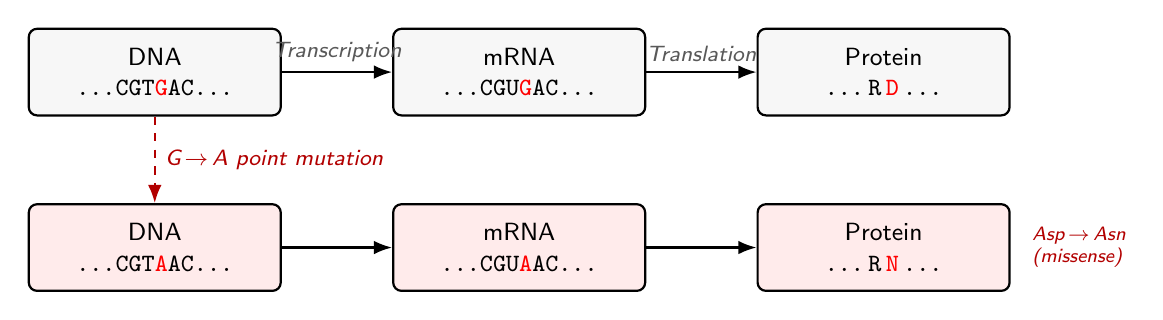
\begin{tikzpicture}[
  font=\sffamily\small,
  box/.style={draw, rounded corners=3pt, minimum width=3.2cm,
    minimum height=1.1cm, align=center, fill=black!3, thick},
  arrow/.style={-Latex, thick},
  tag/.style={font=\sffamily\footnotesize\itshape, text=black!65},
]
  \node[box] (dna)   {DNA \\ \texttt{...CGT\textcolor{red}{\textbf{G}}AC...}};
  \node[box, right=1.4cm of dna]  (mrna)    {mRNA \\ \texttt{...CGU\textcolor{red}{\textbf{G}}AC...}};
  \node[box, right=1.4cm of mrna] (protein) {Protein \\ \texttt{...\,R\,\textcolor{red}{\textbf{D}}\,...}};

  \draw[arrow] (dna) -- node[tag, above] {Transcription} (mrna);
  \draw[arrow] (mrna) -- node[tag, above] {Translation} (protein);

  \node[box, fill=red!8, below=1.1cm of dna]     (dna2)     {DNA \\ \texttt{...CGT\textcolor{red}{\textbf{A}}AC...}};
  \node[box, fill=red!8, right=1.4cm of dna2]    (mrna2)    {mRNA \\ \texttt{...CGU\textcolor{red}{\textbf{A}}AC...}};
  \node[box, fill=red!8, right=1.4cm of mrna2]   (protein2) {Protein \\ \texttt{...\,R\,\textcolor{red}{\textbf{N}}\,...}};

  \draw[arrow] (dna2) -- (mrna2);
  \draw[arrow] (mrna2) -- (protein2);

  \draw[arrow, red!70!black, dashed]
    (dna.south) -- node[tag, right, text=red!70!black] {G\,$\rightarrow$\,A point mutation} (dna2.north);
  \node[tag, right=0.15cm of protein2, text=red!70!black, align=left, font=\sffamily\scriptsize\itshape]
    {Asp\,$\rightarrow$\,Asn \\ (missense)};
\end{tikzpicture}
\caption[The central dogma and a missense mutation]%
{\textbf{The central dogma and the point at which a missense
mutation acts.} The upper row shows the reference sequence: the
codon \texttt{GAC} is transcribed into mRNA and translated to
aspartate (\texttt{D}). The lower row introduces a single-base
substitution (G\,$\rightarrow$\,A) in the DNA that propagates
through transcription to the altered codon \texttt{AAC}, which
the ribosome translates to asparagine (\texttt{N}). The protein
sequence has changed at exactly one position. Whether that change
is benign or pathogenic depends on the structural and functional
context of the affected residue.}
\label{fig:central-dogma}
\end{figure}

A genetic mutation is any permanent alteration in this DNA
template. Mutations are the raw material of biological evolution:
most are neutral, a small proportion are beneficial, and a
clinically important minority disrupt cellular function to the
point of causing disease. The clinical spectrum of mutations
includes single-nucleotide variants (SNVs), small insertions and
deletions (indels), copy-number variations, and large-scale
structural rearrangements \citep{macarthur2014guidelines}. Among
these, the single-nucleotide \emph{missense} variant -- a point
mutation in a protein-coding region that changes one amino acid
to another -- is the most common coding variant in the human
population and the principal focus of this project.

\subsection{Classes of Protein-Coding Variation}
\label{sec:intro-variantclasses}

Within the protein-coding portion of the genome, a single-base
substitution can take one of four functional forms depending on
how the change is read by the genetic code
\citep{alberts2015molecular}:

\begin{description}[style=nextline, leftmargin=2.2em, itemsep=0.25em]
  \item[Synonymous.] The nucleotide change still codes for the
    same amino acid; the protein sequence is unchanged (e.g.\
    \texttt{GCU}\,$\rightarrow$\,\texttt{GCC}, both Ala). These
    are often -- but not always -- clinically silent.
  \item[Missense.] The nucleotide change produces a codon for a
    \emph{different} amino acid (e.g.\
    \texttt{GAC}\,\emph{Asp}\,$\rightarrow$\,\texttt{AAC}\,\emph{Asn}).
    This is the class under study in the present work.
  \item[Nonsense.] The nucleotide change creates a premature stop
    codon (e.g.\ \texttt{UGG}\,\emph{Trp}\,$\rightarrow$\,\texttt{UGA}\,\emph{stop}),
    typically producing a truncated non-functional protein.
  \item[Frameshift.] An insertion or deletion that is not a
    multiple of three shifts the reading frame, scrambling every
    downstream codon.
\end{description}

Missense variants are of special interest because they are
common, they are protein-altering, and their clinical effect is
genuinely uncertain at the individual level. A nonsense variant
in a well-characterised disease gene is almost always pathogenic;
a synonymous variant is almost always benign. A missense variant,
however, can produce anything from a completely wild-type protein
to a catastrophically misfolded one, depending on where the
substitution falls and which amino acid replaces the original.

\subsection{Determinants of Missense Variant Effect}
\label{sec:intro-determinants}

Decades of biochemistry and structural biology have identified
several orthogonal signals that a classifier can, in principle,
learn to exploit \citep{stein2019inferring, guerois2002predicting}:

\begin{enumerate}
  \item \textbf{Evolutionary conservation.} A residue that has
    been invariant across hundreds of millions of years of
    orthologous evolution is almost certainly functionally
    important; substitutions at such positions are more likely
    to be deleterious.
  \item \textbf{Amino-acid chemistry.} A substitution that
    changes charge, hydrophobicity, or volume (e.g.\
    \emph{Arg}\,$\rightarrow$\,\emph{Asp}, reversing the
    side-chain charge) is more likely to disrupt protein
    stability or a binding interface than a conservative
    substitution (e.g.\ \emph{Leu}\,$\rightarrow$\,\emph{Ile}).
  \item \textbf{Structural context.} Substitutions at buried
    core residues, catalytic sites, or secondary-structure
    boundaries are more likely to be pathogenic than those at
    solvent-exposed flexible loops.
  \item \textbf{Gene-level constraint.} Some genes are
    intrinsically intolerant of coding variation across the
    human population; a missense variant in such a gene carries
    stronger prior evidence of pathogenicity than the same
    change in a loss-of-function-tolerant gene
    \citep{karczewski2020gnomad}.
  \item \textbf{Protein-language plausibility.} Modern
    transformer-based protein language models, trained on
    billions of natural protein sequences, assign probabilities
    to each amino acid at each position; substitutions to
    low-probability residues correlate strongly with
    experimental measures of function
    \citep{meier2021language, brandes2023esm1b}.
\end{enumerate}

The five signals are not independent, but their correlation is
imperfect, which is exactly what makes supervised machine
learning an appropriate framework: the classifier learns how to
weigh each signal given labelled examples from \textsc{ClinVar}
and how to combine them non-linearly.

\subsection{Public Reference Resources}
\label{sec:intro-resources}

Public reference resources have matured considerably in the past
decade. \textsc{ClinVar} \citep{landrum2020clinvar} aggregates
variant-disease relationships curated by clinical laboratories
and research groups, using a five-tier pathogenicity scale
(Benign, Likely Benign, Variant of Uncertain Significance,
Likely Pathogenic, Pathogenic). The Genome Aggregation Database
(\textsc{gnomAD}) \citep{karczewski2020gnomad} publishes
population-level allele-frequency and gene-level constraint
metrics derived from more than $140{,}000$ exomes and genomes
across diverse ancestries; its \emph{observed~/~expected} ratio
for missense variation has become the standard measure of how
intolerant a gene is to amino-acid-altering change. The
\textsc{dbNSFP} resource \citep{liu2020dbnsfp} consolidates
dozens of per-variant features including cross-species
conservation (phyloP, GERP\texttt{++}), amino-acid chemistry
descriptors, and predictions from preceding-generation tools.
The existence of these resources makes a supervised
machine-learning approach to missense classification feasible
for a student team, provided one is disciplined about how the
data is combined and evaluated -- precisely the question this
report sets out to address.

\section{Motivation and Significance}
\label{sec:intro-motivation}

Three trends motivate further work in this area. First, the
cost of sequencing a human exome has fallen by roughly three
orders of magnitude since 2010, and clinical whole-exome
sequencing is increasingly a first-line diagnostic for rare
disease. The rate at which \emph{variants} are discovered now
exceeds the rate at which they can be interpreted by human
experts. Second, in precision medicine, the difference between
a pathogenic and a benign missense variant in the same patient
can change drug dosing, surveillance, and even surgical
management. Third, the American College of Medical Genetics and
Genomics (ACMG) standard \citep{richards2015acmg} includes
computational \emph{in silico} evidence among the criteria a
clinical geneticist weighs when classifying a variant, which
means that any tool published in this space must be transparent about
its operating characteristics -- false-positive and
false-negative rates, calibration, and generalisation behaviour.

Against that backdrop, this project sets out to build not
\emph{the highest-scoring} missense classifier but rather
\emph{the most defensible baseline} that a student team can
produce using public data and a modest compute budget. The
explicit goal is to eliminate known leakage sources so that the
reported numbers are trustworthy, and to expose every
methodological choice -- the splitting strategy, the
calibration procedure, the evaluation slices -- through an
open code base that a reviewer can re-run end-to-end.

\section{Problem Statement}
\label{sec:intro-problem}

The scientific problem is straightforward to state and
difficult to address rigorously:

\begin{quote}\itshape
Given a human missense single-nucleotide variant, predict
whether it is pathogenic or benign, accompanied by a
calibrated probability and enough interpretability for a
clinical genetic analyst to audit the prediction.
\end{quote}

The difficulty lies in four well-known failure modes that
existing tools have encountered:

\begin{enumerate}
\item \textbf{Data overload.} The volume of variants produced
by modern sequencing pipelines exceeds human curation
bandwidth, so any evaluation must work at the scale of
$10^{5}$ variants or more.
\item \textbf{Biological complexity.} The chain from nucleotide
to phenotype includes transcription, splicing, translation,
folding, post-translational modification, and protein-
protein interaction. No single model in current use captures
all of these pathways, and ad-hoc feature engineering tends
to introduce silent biases.
\item \textbf{Data contamination.} The most commonly used
benchmark, \textsc{ClinVar}, is also the most commonly used
\emph{calibration target} for published tools. Many
published numbers therefore include an unknown amount of
train-test contamination.
\item \textbf{Evaluation asymmetry.} A model that scores well
on \textsc{ClinVar}-derived tests may collapse to chance
when applied to affected-versus-control \emph{de-novo}
variants from sequencing studies, because the latter
requires gene-level priors that variant-level tools never
see.
\end{enumerate}

\section{Research Questions}
\label{sec:intro-questions}

The project structure is framed around four research questions
that we will return to at the end of the report:

\begin{enumerate}
\item \textbf{RQ1.} How much of the apparent high performance
of a \textsc{ClinVar}-trained classifier is attributable to
specific, removable leakage sources, and how far does the
post-audit number fall once they are eliminated?
\item \textbf{RQ2.} Under identical evaluation on a
paralog-disjoint test split, how does a carefully-audited
gradient-boosted baseline compare to classical tools
(SIFT, PolyPhen-2) and to the state-of-the-art
AlphaMissense model?
\item \textbf{RQ3.} Does the post-audit model generalise to
\textsc{denovo-db} -- a dataset of de-novo variants in
affected children versus unaffected siblings -- and how
much of any gap is closed by adding gene-level constraint
features?
\item \textbf{RQ4.} Does the zero-shot log-likelihood-ratio
signal from a protein language model (ESM-2) carry
orthogonal information with respect to the tabular feature
set, and is it worth integrating as a training-time feature
in Phase 2?
\end{enumerate}

\section{Project Objectives}
\label{sec:intro-objectives}

The concrete objectives guiding the semester of work are:

\begin{itemize}[leftmargin=*,itemsep=0.3em]
\item \textbf{O1.} Assemble a reproducible corpus of missense
variants from \textsc{ClinVar}, \textsc{gnomAD}, and
\textsc{dbNSFP}, filtered to strictly missense rows with
consistent amino-acid fields.
\item \textbf{O2.} Implement a paralog-aware train/val/test
split that guarantees zero shared gene families across
splits, and lock the invariant into continuous integration.
\item \textbf{O3.} Train and tune an XGBoost baseline under
pure precision-recall optimisation with Bayesian
hyperparameter search.
\item \textbf{O4.} Calibrate the classifier with Platt and
isotonic regression, evaluate with the Brier-score
decomposition of Murphy \citep{murphy1973brier}, and report
operating points at clinically relevant recall / precision
targets.
\item \textbf{O5.} Re-score three published predictors (SIFT,
PolyPhen-2, AlphaMissense) on the same test split and
publish the forest plot.
\item \textbf{O6.} Build and evaluate an external-validation
harness on \textsc{denovo-db}, and quantify the effect of
adding gnomAD gene-level constraint features.
\item \textbf{O7.} Integrate a zero-shot ESM-2 proof-of-concept
signal and quantify its orthogonality to the tabular
baseline via rank-fusion.
\item \textbf{O8.} Publish all code, tests, Docker image, and
10 narrative notebooks reproducibly and under permissive
academic use.
\end{itemize}

\section{Scope and Boundaries}
\label{sec:intro-scope}

We restrict scope in several deliberate ways:

\begin{itemize}
\item The classification target is a \emph{binary} label
(pathogenic versus benign). We do not attempt to reproduce
the five-class \textsc{ClinVar} scheme (benign, likely
benign, VUS, likely pathogenic, pathogenic); the
variants-of-uncertain-significance (VUS) class would
require a fundamentally different loss function.
\item Only \emph{missense} SNVs are considered. Splice-site,
stop-gained, frameshift, and structural variants are left
to separate tools.
\item Only \textsc{GRCh38} coordinates are supported. This
choice is driven by the fact that our primary feature
source (\textsc{dbNSFP} 5.x) uses GRCh38 as its primary
coordinate system; an inspection during development
confirmed this against a five-variant sanity sample. The
external dataset \textsc{denovo-db} is handled through a
separate GRCh37-aware code path.
\item Compute is limited to a consumer laptop with Apple MPS
acceleration for ESM-2 zero-shot experiments and one free
Colab T4 GPU session for full-training-set ESM-2
scoring. No institutional GPU cluster is used.
\end{itemize}

\section{Key Contributions}
\label{sec:intro-contributions}

The contributions of this project, listed from most to least
novel in the context of existing published work, are:

\begin{enumerate}
\item \textbf{A transparent leakage audit with before-and-after
numbers} for a missense classifier, showing that a
difference of 0.117 PR-AUC between a na\"ive and a
defensible pipeline is fully attributable to three
removable sources.
\item \textbf{A re-scoring of SIFT, PolyPhen-2, and
AlphaMissense on our own paralog-disjoint test split},
enabling a like-for-like comparison that is rarely
presented in this literature.
\item \textbf{An external validation on \textsc{denovo-db}}
with pre- and post-gnomAD-constraint numbers, showing
that gene-level priors close approximately half the
generalisation gap on unseen gene families.
\item \textbf{A zero-shot ESM-2 proof-of-concept}
establishing that the protein-language-model log-
likelihood-ratio provides orthogonal signal under rank-
fusion, which motivates the Phase-2 full-training-set
integration currently running on Colab.
\item \textbf{A fully reproducible code base} -- 158 tests,
CI-enforced leakage gate, pinned dependencies, Docker
image, 10 narrative Jupyter notebooks, a Streamlit demo,
and this LaTeX report -- that a future student could
extend without reverse-engineering.
\end{enumerate}

\section{Report Organisation}
\label{sec:intro-org}

Chapter~\ref{ch:related} surveys the prior-art
predictors that define our comparison baseline.
Chapter~\ref{ch:framework} presents the system framework,
feasibility analyses, and the three-part pipeline at the
design level. Chapter~\ref{ch:analysis} develops the full
set of system requirements and accompanies them with the
six standard UML diagrams and the interface design.
Chapter~\ref{ch:implementation} reports the concrete
implementation, results, and the comparison tables.
Chapter~\ref{ch:conclusion} concludes and lays out the
Phase-2 roadmap. Three appendices provide extended results
tables, selected code listings, and the environment /
reproducibility specification.

% ═════════════════════════════════════════════════════════════════════════
%   CHAPTER 2 — RELATED WORKS
% ═════════════════════════════════════════════════════════════════════════

\chapter{Related Works}
\label{ch:related}

\section{Introduction}
\label{sec:rw-intro}

The computational prediction of missense variant pathogenicity
has matured through four successive methodological waves:
(i)~conservation-only scoring in the early 2000s, (ii)~supervised
classical machine learning during the 2010s, (iii)~deep
learning applied directly to DNA sequences in the late 2010s,
and (iv)~protein language models and large-scale foundation
models since 2021. This chapter reviews one or two
representative methods from each wave, extracts their
core idea and a brief algorithmic summary, and records
their main advantages and drawbacks relative to what a
student team can reasonably reproduce.

\section{Problem Scope}
\label{sec:rw-scope}

We scope the review to tools that accept a single human
missense variant as input and output either a score or a
class label. Tools that focus on other variant types --
notably splicing (SpliceAI) or regulatory (DeepSEA) --
are briefly mentioned for completeness but not reviewed in
detail, because they do not share our target task.

\section{Literature Review}
\label{sec:rw-literature}

The following eight subsections review one or two representative
methods from each historical wave. Every subsection follows the
same structure -- core idea, algorithmic summary, formal
description where useful, a schematic figure drawn in TikZ, and
a bullet-list discussion of strengths and weaknesses relative
to the benchmark on which we ultimately evaluate.

% ───────────────────────── SIFT ─────────────────────────
\subsection{SIFT (2003) \texorpdfstring{\citep{ng2003sift}}{(Ng and Henikoff, 2003)}}
\label{sec:rw-sift}

\textbf{Core idea.} SIFT (\emph{Sorting Intolerant From Tolerant})
was the first widely-deployed computational tool for
missense pathogenicity prediction. It rests on a single
hypothesis: an amino-acid position that has remained
invariant across evolutionary time tolerates few
substitutions, so a variant at such a position is more
likely to be deleterious than a variant at a fast-
evolving position \citep{ng2003sift}.

\textbf{Algorithmic summary.} For a query variant,
SIFT retrieves a multiple sequence alignment (MSA) of
the target protein and its homologues, computes a
position-specific amino-acid probability matrix, and
assigns a score $s \in [0, 1]$ by normalising the
observed frequency of the alternate amino acid against
the most-observed amino acid at that position. The
algorithm's full decision logic can be summarised as:

\[
s_i(a) \;=\; \frac{p_i(a)}{\max_{a' \in \mathcal{A}_{20}} p_i(a')}
\qquad\text{with}\qquad
\text{label} = \begin{cases}
\text{intolerant}  & s_i(a) < 0.05 \\
\text{tolerated} & s_i(a) \geq 0.05
\end{cases}
\]

where $p_i(a)$ is the Dirichlet-smoothed frequency of
amino acid $a$ at column $i$ of the MSA.
Figure~\ref{fig:sift-pipeline} summarises the pipeline.

\begin{figure}[htbp]
\centering
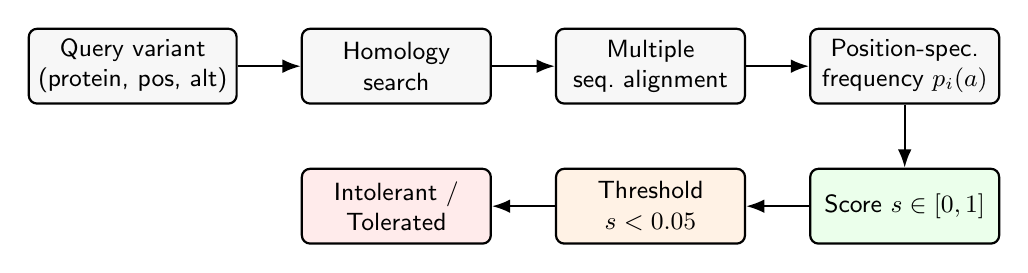
\begin{tikzpicture}[
  font=\sffamily\small,
  box/.style={draw, rounded corners=3pt, minimum width=2.4cm,
    minimum height=0.95cm, align=center, fill=black!3, thick},
  arrow/.style={-Latex, thick},
]
  \node[box] (var)     {Query variant \\ (protein, pos, alt)};
  \node[box, right=0.8cm of var] (homo)   {Homology \\ search};
  \node[box, right=0.8cm of homo] (msa)    {Multiple \\ seq.\ alignment};
  \node[box, right=0.8cm of msa] (mat)    {Position-spec.\ \\ frequency $p_i(a)$};
  \node[box, below=0.8cm of mat, fill=green!8] (score)  {Score $s \in [0,1]$};
  \node[box, left=0.8cm of score, fill=orange!10] (thr)  {Threshold \\ $s < 0.05$};
  \node[box, left=0.8cm of thr, fill=red!8]   (out)   {Intolerant / \\ Tolerated};

  \draw[arrow] (var) -- (homo);
  \draw[arrow] (homo) -- (msa);
  \draw[arrow] (msa) -- (mat);
  \draw[arrow] (mat) -- (score);
  \draw[arrow] (score) -- (thr);
  \draw[arrow] (thr) -- (out);
\end{tikzpicture}
\caption[SIFT pipeline]{\textbf{SIFT pipeline.} From a missense
variant, a homology-search step gathers orthologues which are
aligned into a multiple sequence alignment. A position-specific
frequency matrix is computed and the alternate amino acid is
scored relative to the most-observed amino acid at that
column. A hard threshold of $0.05$ produces a binary label.}
\label{fig:sift-pipeline}
\end{figure}

\textbf{Advantages.}
\begin{itemize}[leftmargin=2em, itemsep=0.15em]
  \item Mature (over two decades of clinical deployment) and
    trivially accessible through Ensembl's Variant Effect
    Predictor (VEP) REST API.
  \item No supervised training data is required; the score
    is a deterministic function of the input alignment.
  \item Low compute requirement; scores can be produced
    on a laptop in minutes for any human gene.
\end{itemize}

\textbf{Disadvantages.}
\begin{itemize}[leftmargin=2em, itemsep=0.15em]
  \item Ignores amino-acid chemistry entirely: a conservative
    substitution (e.g.\ Leu\,$\rightarrow$\,Ile) and a
    radical one (e.g.\ Arg\,$\rightarrow$\,Asp) receive the
    same score if the alignment frequencies are identical.
  \item Depends heavily on alignment quality, which is poor
    in intrinsically disordered regions and for genes with
    few annotated homologues.
  \item The binary threshold of $0.05$ is arbitrary and
    produces poor calibration for ACMG-style clinical
    reporting.
\end{itemize}

% ───────────────────────── PolyPhen-2 ─────────────────────────
\subsection{PolyPhen-2 (2010) \texorpdfstring{\citep{adzhubei2010polyphen}}{(Adzhubei et al., 2010)}}
\label{sec:rw-polyphen}

\textbf{Core idea.} PolyPhen-2 (\emph{Polymorphism
Phenotyping, version 2}) was the first widely-adopted
\emph{supervised} classifier for missense pathogenicity
\citep{adzhubei2010polyphen}. It combines conservation
with amino-acid chemistry and limited structural
context, trained on two internally-curated datasets
(\textsc{HumDiv}, 23k variants, and \textsc{HumVar},
13k variants).

\textbf{Algorithmic summary.} Eleven features are
extracted per variant: three sequence-based features
(including the PSIC conservation score), six
structural features derived from aligned PDB entries
(e.g.\ solvent accessibility, crystallographic
B-factor, secondary structure), and two annotation
features from Pfam domains. A na\"ive Bayes classifier
returns a posterior $P(\text{damaging} \mid \mathbf{x})$
and assigns one of three labels: \emph{benign},
\emph{possibly damaging}, or \emph{probably damaging}.

\begin{figure}[htbp]
\centering
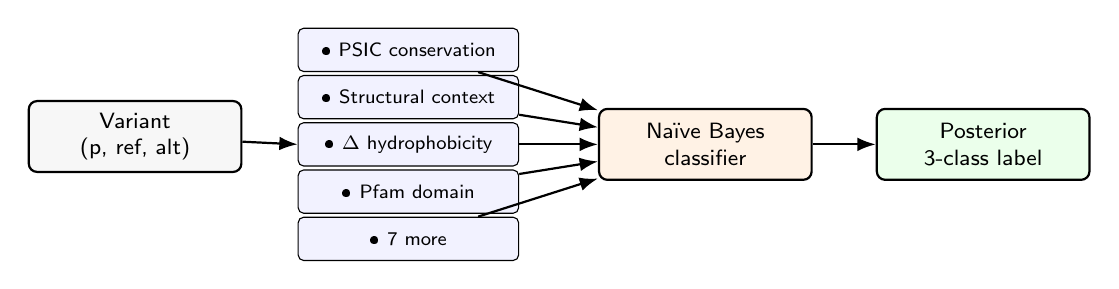
\begin{tikzpicture}[
  font=\sffamily\footnotesize,
  box/.style={draw, rounded corners=3pt, minimum width=2.7cm,
    minimum height=0.9cm, align=center, fill=black!3, thick},
  feat/.style={draw, rounded corners=2pt, minimum width=2.8cm,
    minimum height=0.55cm, align=left, fill=blue!5, font=\sffamily\scriptsize},
  arrow/.style={-Latex, thick},
]
  \node[box] (var)   {Variant \\ (p, ref, alt)};
  \node[feat, right=0.7cm of var, yshift=1.1cm]  (f1)    {\textbullet\ PSIC conservation};
  \node[feat, right=0.7cm of var, yshift=0.5cm]  (f2)    {\textbullet\ Structural context};
  \node[feat, right=0.7cm of var, yshift=-0.1cm] (f3)    {\textbullet\ $\Delta$ hydrophobicity};
  \node[feat, right=0.7cm of var, yshift=-0.7cm] (f4)    {\textbullet\ Pfam domain};
  \node[feat, right=0.7cm of var, yshift=-1.3cm] (f5)    {\textbullet\ 7 more};
  \node[box, right=1.0cm of f3, fill=orange!10] (nb)   {Na\"ive Bayes \\ classifier};
  \node[box, right=0.8cm of nb, fill=green!8]  (out)   {Posterior \\ 3-class label};

  \draw[arrow] (var) -- (f3.west);
  \draw[arrow] (f1) -- (nb);
  \draw[arrow] (f2) -- (nb);
  \draw[arrow] (f3) -- (nb);
  \draw[arrow] (f4) -- (nb);
  \draw[arrow] (f5) -- (nb);
  \draw[arrow] (nb) -- (out);
\end{tikzpicture}
\caption[PolyPhen-2 pipeline]{\textbf{PolyPhen-2.} Eleven
hand-crafted features are extracted from conservation,
structural, and annotation sources, and a na\"ive Bayes
classifier trained on \textsc{HumDiv} maps the feature vector to
a three-way label.}
\label{fig:polyphen-pipeline}
\end{figure}

\textbf{Advantages.}
\begin{itemize}[leftmargin=2em, itemsep=0.15em]
  \item Incorporates amino-acid chemistry and limited
    structural context -- a distinct methodological step
    beyond conservation alone.
  \item Three-way output is more clinically useful than
    SIFT's binary label; is widely adopted in ACMG-adjacent
    workflows.
\end{itemize}

\textbf{Disadvantages.}
\begin{itemize}[leftmargin=2em, itemsep=0.15em]
  \item Training labels originate from \textsc{Swiss-Var}
    and \textsc{HumDiv}, which partially overlap
    \textsc{ClinVar}; benchmarks evaluated on
    \textsc{ClinVar} therefore carry a contamination risk.
  \item Posterior probabilities are not calibrated: the
    reported confidence intervals do not match empirical
    frequencies.
  \item The feature set is static; re-training the model on
    new data is laborious because of dependence on
    external PDB alignments.
\end{itemize}

% ───────────────────────── REVEL ─────────────────────────
\subsection{REVEL (2016) \texorpdfstring{\citep{ioannidis2016revel}}{(Ioannidis et al., 2016)}}
\label{sec:rw-revel}

\textbf{Core idea.} REVEL (\emph{Rare Exome Variant
Ensemble Learner}) is an ensemble meta-classifier that
\emph{stacks} thirteen preceding-generation tools --
CADD, PolyPhen-2, SIFT, MutationTaster, MutationAssessor,
FATHMM, LRT, GERP\texttt{++}, and others -- using a
random forest meta-learner. By construction it exploits
signal that no single base learner captures
\citep{ioannidis2016revel}.

\textbf{Algorithmic summary.} For each missense variant,
REVEL extracts a 13-dimensional feature vector
$\mathbf{z} = (z_1, \dots, z_{13})$ where $z_k$ is the
score of the $k$-th base tool. A random forest with
$1{,}000$ trees, trained on a curated set of rare
disease variants versus rare neutral variants, returns
$\widehat{P}(\text{pathogenic} \mid \mathbf{z}) \in [0,1]$.

\begin{figure}[htbp]
\centering
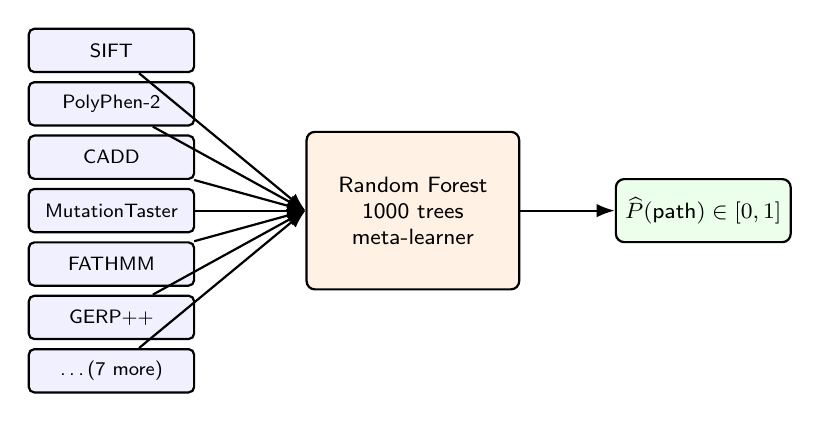
\begin{tikzpicture}[
  font=\sffamily\footnotesize,
  base/.style={draw, rounded corners=2pt, minimum width=2.1cm,
    minimum height=0.55cm, align=center, fill=blue!6, thick,
    font=\sffamily\scriptsize},
  rf/.style={draw, rounded corners=3pt, minimum width=2.7cm,
    minimum height=2cm, align=center, fill=orange!10, thick},
  outbox/.style={draw, rounded corners=3pt, minimum width=2.2cm,
    minimum height=0.8cm, align=center, fill=green!8, thick},
  arrow/.style={-Latex, thick},
]
  \node[base] (t1) {SIFT};
  \node[base, below=0.1cm of t1] (t2) {PolyPhen-2};
  \node[base, below=0.1cm of t2] (t3) {CADD};
  \node[base, below=0.1cm of t3] (t4) {MutationTaster};
  \node[base, below=0.1cm of t4] (t5) {FATHMM};
  \node[base, below=0.1cm of t5] (t6) {GERP++};
  \node[base, below=0.1cm of t6] (t7) {\ldots (7 more)};

  \node[rf, right=1.4cm of t4] (rf) {Random Forest \\ 1000 trees \\ meta-learner};
  \node[outbox, right=1.2cm of rf] (out) {$\widehat{P}(\text{path}) \in [0,1]$};

  \foreach \t in {t1,t2,t3,t4,t5,t6,t7}{
    \draw[arrow] (\t) -- (rf.west);
  }
  \draw[arrow] (rf) -- (out);
\end{tikzpicture}
\caption[REVEL pipeline]{\textbf{REVEL stacks 13 base
predictors.} Each base predictor produces its own score on
the query variant; the random-forest meta-learner combines
these into a calibrated pathogenicity probability.}
\label{fig:revel-pipeline}
\end{figure}

\textbf{Advantages.}
\begin{itemize}[leftmargin=2em, itemsep=0.15em]
  \item Empirically strong on \textsc{ClinVar} benchmarks,
    with reported ROC-AUC around $0.94$ at release.
  \item Distributed through \textsc{dbNSFP}, so querying a
    variant costs a single table lookup.
\end{itemize}

\textbf{Disadvantages.}
\begin{itemize}[leftmargin=2em, itemsep=0.15em]
  \item Several base predictors (PolyPhen-2, CADD) were
    themselves trained on variants that overlap
    \textsc{ClinVar}, producing \emph{compound
    contamination} when REVEL is evaluated on
    \textsc{ClinVar}. The paper's reported numbers are
    therefore upper-bound estimates.
  \item Does not ship well-calibrated probabilities;
    threshold selection for ACMG interpretation is left
    to the user.
  \item The 13 base tools must all be re-run for any variant
    not already in \textsc{dbNSFP}, limiting deployment
    flexibility.
\end{itemize}

% ───────────────────────── CADD ─────────────────────────
\subsection{CADD (2014--2019) \texorpdfstring{\citep{rentzsch2019cadd}}{(Rentzsch et al., 2019)}}
\label{sec:rw-cadd}

\textbf{Core idea.} Combined Annotation-Dependent
Depletion (CADD) side-steps the training-label scarcity
problem by framing pathogenicity prediction as a
\emph{supervised selection task}. Training examples are
generated from two sources: observed human variants (as
the ``derived'' class, presumed to be under relaxed
selection) and simulated de-novo variants from a neutral
mutation model (as the ``simulated'' class). A
classifier trained to discriminate the two implicitly
learns signatures of purifying selection
\citep{rentzsch2019cadd}.

\textbf{Algorithmic summary.} For each position in the
human genome, CADD extracts a large feature vector
(initially $63$ features; the v1.6 release uses more
than $1{,}400$ features spanning conservation,
regulatory annotations, transcript structure, and
protein-level features). A logistic regression (v1.0)
or random forest (v1.4\texttt{+}) is trained to assign
higher scores to simulated variants than to observed
ones. The output is a raw classification score that
is converted to a phred-like scaled score,
\[
\text{CADD}_{\text{phred}} = -10 \log_{10}\!
\Bigl( \text{rank}(v)\,/\,N_{\text{total}} \Bigr),
\]
where $v$ is the variant and $N_{\text{total}}$ is the
total number of variants scored genome-wide.

\begin{figure}[htbp]
\centering
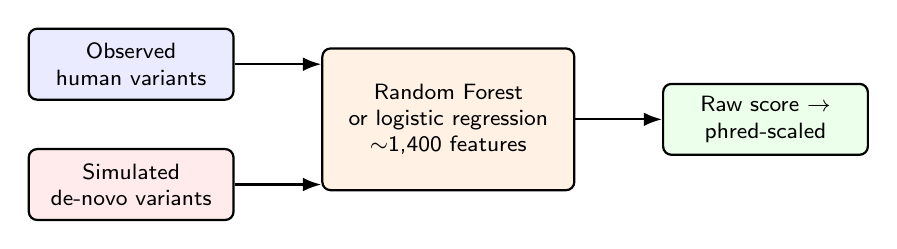
\begin{tikzpicture}[
  font=\sffamily\footnotesize,
  box/.style={draw, rounded corners=3pt, minimum width=2.6cm,
    minimum height=0.9cm, align=center, fill=black!3, thick},
  arrow/.style={-Latex, thick},
]
  \node[box, fill=blue!8] (obs)  {Observed\\human variants};
  \node[box, fill=red!8, below=0.6cm of obs] (sim) {Simulated\\de-novo variants};
  \node[box, right=1.1cm of obs, yshift=-0.7cm, minimum height=1.8cm,
    minimum width=3.2cm, fill=orange!10] (rf) {Random Forest\\or logistic regression\\$\sim$1{,}400 features};
  \node[box, right=1.1cm of rf, fill=green!8] (out) {Raw score $\rightarrow$\\phred-scaled};

  \draw[arrow] (obs.east) -- (rf.west |- obs.east);
  \draw[arrow] (sim.east) -- (rf.west |- sim.east);
  \draw[arrow] (rf) -- (out);
\end{tikzpicture}
\caption[CADD pipeline]{\textbf{CADD training.} A classifier
is trained to distinguish observed human variants from
simulated de-novo variants across the whole genome. The
trained discriminator implicitly ranks novel positions by
the strength of purifying selection; the raw output is
phred-transformed for reporting.}
\label{fig:cadd-pipeline}
\end{figure}

\textbf{Advantages.}
\begin{itemize}[leftmargin=2em, itemsep=0.15em]
  \item Does not require clinical pathogenicity labels,
    so \textsc{ClinVar} contamination is not an issue.
  \item Whole-genome coverage -- a single score per
    base pair -- supports non-coding analyses.
\end{itemize}

\textbf{Disadvantages.}
\begin{itemize}[leftmargin=2em, itemsep=0.15em]
  \item The simulated null is an imperfect proxy for
    neutrality; sites under weak selection are scored
    similarly to sites under strong selection.
  \item Raw logits and phred-transformed scores are not
    calibrated probabilities, so clinical thresholding
    is subjective.
  \item Performance on missense variants is below that
    of supervised missense-specific tools (ROC-AUC
    $\sim 0.82$ on \textsc{ClinVar} missense subsets).
\end{itemize}

% ───────────────────────── VARITY ─────────────────────────
\subsection{VARITY (2021) \texorpdfstring{\citep{wu2021varity}}{(Wu et al., 2021)}}
\label{sec:rw-varity}

\textbf{Core idea.} VARITY addresses an often-overlooked
weakness of supervised missense tools: the training
labels are themselves noisy. A label of \emph{likely
benign} in \textsc{ClinVar} may reflect limited
evidence rather than confirmed benignity. VARITY
introduces a \emph{sample-reweighting} scheme in which
training examples are weighted by an estimated label-
confidence score, so that high-confidence examples
dominate the XGBoost loss
\citep{wu2021varity}.

\textbf{Algorithmic summary.} The training set is
\textsc{HumsaVar} plus a curated set of multiplex-assay
measurements (typically variant-effect deep mutational
scans). Each example $(x_i, y_i)$ receives a weight
$w_i$ that increases with assay replication and decreases
with label discordance among secondary sources. XGBoost
minimises the weighted logistic loss
$\mathcal{L} = -\sum_i w_i\, [\, y_i \log \hat{y}_i +
(1 - y_i)\log(1 - \hat{y}_i)\,]$ with standard
boosting hyperparameters.

\textbf{Advantages.}
\begin{itemize}[leftmargin=2em, itemsep=0.15em]
  \item Principled handling of label noise -- a legitimate
    methodological contribution.
  \item Published model card with feature-importance plots
    and reported confidence intervals.
\end{itemize}

\textbf{Disadvantages.}
\begin{itemize}[leftmargin=2em, itemsep=0.15em]
  \item Gene-level (not paralog-level) splits, so
    \textsc{VARITY}'s own benchmark is still at risk from
    paralog leakage of the type we address in
    Chapter~\ref{ch:implementation}.
  \item No external validation on de-novo cohorts is
    reported in the original paper.
\end{itemize}

% ───────────────────────── EVE ─────────────────────────
\subsection{EVE (2021) \texorpdfstring{\citep{frazer2021eve}}{(Frazer et al., 2021)}}
\label{sec:rw-eve}

\textbf{Core idea.} EVE (\emph{Evolutionary model of
Variant Effect}) takes a purely unsupervised route:
for each protein of interest, a variational auto-encoder
(VAE) is fit to the protein's own multiple sequence
alignment, effectively modelling the probability density
over natural variants seen across evolution
\citep{frazer2021eve}. At inference time, the evidence
lower bound (ELBO) of a candidate variant relative to
the wild-type supplies a pathogenicity score:
\[
s_{\text{EVE}}(v) \;=\; \mathrm{ELBO}(v) - \mathrm{ELBO}(v_{\text{wt}}).
\]

\begin{figure}[htbp]
\centering
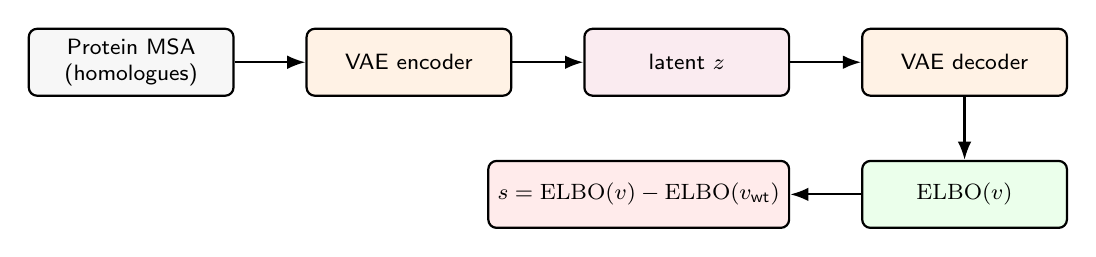
\begin{tikzpicture}[
  font=\sffamily\footnotesize,
  box/.style={draw, rounded corners=3pt, minimum width=2.6cm,
    minimum height=0.85cm, align=center, fill=black!3, thick},
  arrow/.style={-Latex, thick},
]
  \node[box] (msa)    {Protein MSA \\ (homologues)};
  \node[box, right=0.9cm of msa, fill=orange!10] (enc)   {VAE encoder};
  \node[box, right=0.9cm of enc, fill=purple!8]  (z)   {latent $z$};
  \node[box, right=0.9cm of z, fill=orange!10]   (dec)   {VAE decoder};
  \node[box, below=0.8cm of dec, fill=green!8]  (elbo)    {$\mathrm{ELBO}(v)$};
  \node[box, left=0.9cm of elbo, fill=red!8]     (score)  {$s = \mathrm{ELBO}(v) - \mathrm{ELBO}(v_\text{wt})$};

  \draw[arrow] (msa) -- (enc);
  \draw[arrow] (enc) -- (z);
  \draw[arrow] (z)   -- (dec);
  \draw[arrow] (dec) -- (elbo);
  \draw[arrow] (elbo) -- (score);
\end{tikzpicture}
\caption[EVE pipeline]{\textbf{EVE.} A per-gene VAE is trained
on the protein's multiple-sequence alignment; the ELBO of a
test variant relative to the wild-type acts as a pathogenicity
score. No ClinVar supervision is used.}
\label{fig:eve-pipeline}
\end{figure}

\textbf{Advantages.}
\begin{itemize}[leftmargin=2em, itemsep=0.15em]
  \item Fully unsupervised: never touches \textsc{ClinVar}
    at any training or calibration step, so is
    contamination-proof by construction.
  \item Per-gene specialisation gives strong performance
    on the subset of genes where the alignment is deep.
\end{itemize}

\textbf{Disadvantages.}
\begin{itemize}[leftmargin=2em, itemsep=0.15em]
  \item Coverage limited to approximately $3{,}000$ genes
    at the original release; building an alignment is
    labour-intensive for many clinically-relevant genes.
  \item Per-gene training cost is high; scaling to the
    whole proteome is impractical for a student team.
  \item The ELBO is not a calibrated probability; users
    must map it through a threshold that the paper does
    not fully specify.
\end{itemize}

% ───────────────────────── ESM-1b / ESM-2 ─────────────────────────
\subsection{ESM-1b / ESM-2 zero-shot (2023)
  \texorpdfstring{\citep{brandes2023esm1b, lin2023esm2}}{(Brandes et al., 2023; Lin et al., 2023)}}
\label{sec:rw-esm}

\textbf{Core idea.} Large transformer-based protein
language models, trained with a masked-amino-acid
objective on UniRef50 or UniRef90, learn position-
specific distributions over all twenty canonical amino
acids conditioned on their sequence context. For a
missense variant, the log-likelihood ratio (LLR)
\[
\mathrm{LLR}(v) \;=\;
\log p(a_{\text{alt}} \mid \text{context}) \;-\;
\log p(a_{\text{ref}} \mid \text{context})
\]
ranks substitutions by how \emph{implausible} they are
in natural protein space
\citep{brandes2023esm1b, meier2021language}. The model
is never fine-tuned on \textsc{ClinVar}, so the score
is strictly zero-shot.

\begin{figure}[htbp]
\centering
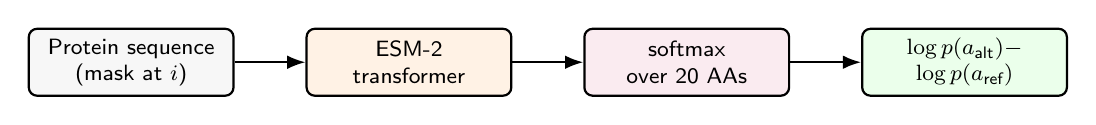
\begin{tikzpicture}[
  font=\sffamily\footnotesize,
  box/.style={draw, rounded corners=3pt, minimum width=2.6cm,
    minimum height=0.85cm, align=center, fill=black!3, thick},
  arrow/.style={-Latex, thick},
]
  \node[box] (seq)      {Protein sequence \\ (mask at $i$)};
  \node[box, right=0.9cm of seq, fill=orange!10] (esm)  {ESM-2 \\ transformer};
  \node[box, right=0.9cm of esm, fill=purple!8]  (sm)   {softmax \\ over 20 AAs};
  \node[box, right=0.9cm of sm, fill=green!8]    (llr)  {$\log p(a_\text{alt}) - $\\$\log p(a_\text{ref})$};

  \draw[arrow] (seq) -- (esm);
  \draw[arrow] (esm) -- (sm);
  \draw[arrow] (sm)  -- (llr);
\end{tikzpicture}
\caption[ESM-2 zero-shot LLR]{\textbf{ESM-2 zero-shot scoring.}
The variant position is masked, a single transformer
forward pass produces the softmax over the 20 canonical
amino acids, and the log-likelihood ratio of the alternate
vs reference residue is reported.}
\label{fig:esm2-pipeline}
\end{figure}

\textbf{Advantages.}
\begin{itemize}[leftmargin=2em, itemsep=0.15em]
  \item Fully general: covers the whole human proteome
    (all $\sim$20{,}000 proteins) with a single model.
  \item Provably uncontaminated by \textsc{ClinVar} --
    the training objective is masked reconstruction on
    UniRef, not pathogenicity classification.
  \item The 35M-parameter \texttt{esm2\_t12\_35M\_UR50D}
    model fits on a single consumer GPU, enabling
    academic reproduction.
\end{itemize}

\textbf{Disadvantages.}
\begin{itemize}[leftmargin=2em, itemsep=0.15em]
  \item Moderate standalone discrimination
    (reported ROC-AUC around $0.85$ on \textsc{ClinVar}).
  \item Requires a per-variant forward pass; scoring a
    quarter-million variants is GPU-hours of compute.
  \item The raw LLR is not a calibrated probability;
    combining it with supervised features benefits from
    a downstream fusion step (which we evaluate in
    Section~\ref{sec:exp-rankfusion}).
\end{itemize}

% ───────────────────────── AlphaMissense ─────────────────────────
\subsection{AlphaMissense (2023) \texorpdfstring{\citep{cheng2023alphamissense}}{(Cheng et al., 2023)}}
\label{sec:rw-am}

\textbf{Core idea.} AlphaMissense is the current
state-of-the-art system for missense pathogenicity
prediction on \textsc{ClinVar}-style benchmarks. It
fine-tunes an \textsc{AlphaFold}-style structural
representation with a masked-amino-acid objective and
calibrates the output against \textsc{ClinVar} labels
at release \citep{cheng2023alphamissense}. The system
was trained using Google-scale TPU resources and is
distributed as a pre-computed score table covering
every possible human missense variant.

\begin{figure}[htbp]
\centering
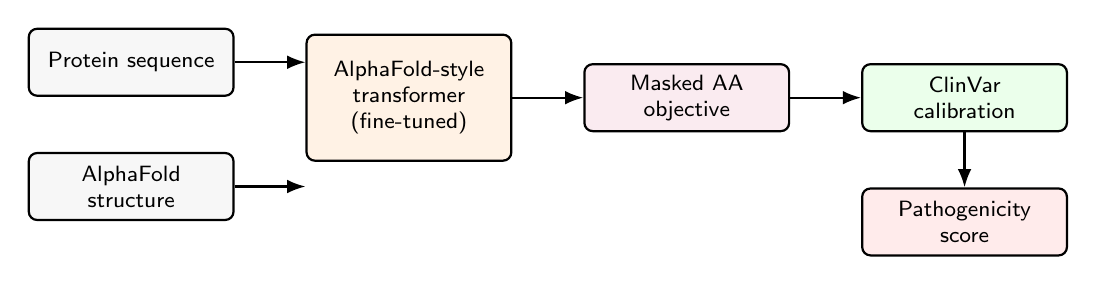
\begin{tikzpicture}[
  font=\sffamily\footnotesize,
  box/.style={draw, rounded corners=3pt, minimum width=2.6cm,
    minimum height=0.85cm, align=center, fill=black!3, thick},
  arrow/.style={-Latex, thick},
]
  \node[box] (seq)      {Protein sequence};
  \node[box, below=0.7cm of seq]  (struct)  {AlphaFold \\ structure};
  \node[box, right=0.9cm of seq, yshift=-0.45cm, fill=orange!10, minimum height=1.6cm] (fm) {AlphaFold-style\\transformer\\(fine-tuned)};
  \node[box, right=0.9cm of fm, fill=purple!8]    (maa)   {Masked AA \\ objective};
  \node[box, right=0.9cm of maa, fill=green!8]    (cal)   {ClinVar \\ calibration};
  \node[box, below=0.7cm of cal, fill=red!8]     (out)   {Pathogenicity \\ score};

  \draw[arrow] (seq.east) -- (fm.west |- seq.east);
  \draw[arrow] (struct.east) -- (fm.west |- struct.east);
  \draw[arrow] (fm) -- (maa);
  \draw[arrow] (maa) -- (cal);
  \draw[arrow] (cal) -- (out);
\end{tikzpicture}
\caption[AlphaMissense pipeline]{\textbf{AlphaMissense.}
Sequence and AlphaFold structural features are fed to a
fine-tuned transformer trained with a masked-amino-acid
objective. The raw output is calibrated against
\textsc{ClinVar} before release.}
\label{fig:am-pipeline}
\end{figure}

\textbf{Advantages.}
\begin{itemize}[leftmargin=2em, itemsep=0.15em]
  \item State-of-the-art \textsc{ClinVar} benchmark
    performance (reported PR-AUC around $0.94$).
  \item Covers the full human proteome as a pre-computed
    table; a variant lookup is $O(1)$.
\end{itemize}

\textbf{Disadvantages.}
\begin{itemize}[leftmargin=2em, itemsep=0.15em]
  \item Training and calibration both use
    \textsc{ClinVar}, so evaluation on any
    \textsc{ClinVar}-derived benchmark contains an
    irreducible contamination risk: the reported gap
    between AlphaMissense and its competitors is a
    mix of methodological improvement and benchmark
    overlap.
  \item Reproduction is out of reach for academic teams
    (TPU-pod scale training budget).
  \item Distributed as a score table without the underlying
    model weights, limiting methodological inspection
    and external validation.
\end{itemize}

% ───────────────────────── Consolidated comparison ─────────────────────────
\subsection{Consolidated Comparison}
\label{sec:rw-consolidated}

Table~\ref{tab:rw-consolidated} synthesises the eight
reviewed methods along six axes relevant to a
methodologically honest evaluation: supervision,
\textsc{ClinVar} contamination risk, split strategy
used at publication, calibration, paralog guard, and
reported external-cohort validation.

\begin{table}[htbp]
\centering
\caption[Related-work consolidated comparison]{
Consolidated comparison of the eight reviewed missense
pathogenicity predictors. \emph{Supervision} indicates
whether the model consumes clinical pathogenicity labels
during training. \emph{Clinvar risk} summarises whether
the published benchmark is at risk of training-set
contamination. \emph{Paralog guard} indicates whether
the publication reports an evaluation free of paralog
leakage. \emph{External?} indicates whether the paper
validates on a cohort not derived from \textsc{ClinVar}
(e.g.\ \textsc{denovo-db}, ProteinGym).}
\label{tab:rw-consolidated}
\footnotesize
\renewcommand{\arraystretch}{1.2}
\resizebox{\linewidth}{!}{%
\begin{tabular}{@{} l c c c c c c @{}}
\toprule
\textbf{Method} & \textbf{Year} & \textbf{Supervision}
 & \textbf{ClinVar risk} & \textbf{Calibration}
 & \textbf{Paralog guard} & \textbf{External?} \\
\midrule
SIFT           & 2003 & unsup.\  & none    & --          & --   & --   \\
PolyPhen-2     & 2010 & sup.\    & partial & soft        & --   & --   \\
CADD           & 2014+ & self-sup.\ & none    & phred      & --   & --   \\
REVEL          & 2016 & sup.\    & compound& --          & --   & --   \\
VARITY         & 2021 & sup.\    & partial & reported    & gene & --   \\
EVE            & 2021 & unsup.\  & none    & ELBO only   & gene & partial \\
ESM-1b/ESM-2   & 2023 & zero-shot& none    & --          & --   & partial \\
AlphaMissense  & 2023 & sup.\    & high    & calibrated  & gene & --   \\
\midrule
\textbf{This work} & \textbf{2026} & \textbf{sup.+zs fusion}
 & \textbf{audited} & \textbf{isotonic} & \textbf{paralog family}
 & \textbf{denovo-db} \\
\bottomrule
\end{tabular}%
}
\end{table}

\section{Research Gap}
\label{sec:rw-gap}

Two observations motivate our methodological choices.
First, most published tools do not evaluate against a
\emph{paralog-aware} test split, even though strongly
similar paralogs (such as the 109 keratin members or 83
cadherin members) can produce optimistically biased
benchmarks when split only at the gene level. Second,
almost no published tool reports external validation on
a dataset not derived from \textsc{ClinVar}: the near-
chance performance of tabular classifiers on
\textsc{denovo-db} is simply not present in most paper
tables. The project's methodological focus lives in
exactly those two gaps.

\section{Project Contribution}
\label{sec:rw-contribution}

Our project closes both gaps concretely. We implement a
paralog-aware split with zero shared gene families
between train/val/test (verified by continuous
integration on every push), and we evaluate on
\textsc{denovo-db} in addition to the paralog-disjoint
\textsc{ClinVar} test. We then quantify the specific
value of gene-level gnomAD constraint features on the
de-novo generalisation task, reporting pre- and
post-constraint numbers separately, and we publish the
first end-to-end like-for-like comparison of our baseline
against SIFT, PolyPhen-2, and AlphaMissense under a
single identical evaluation.

\section{Summary}
\label{sec:rw-summary}

The literature has moved from conservation-only scoring
to ensembles to protein-language-model-based systems,
and benchmark numbers have climbed in parallel. The
distance between these numbers and the real-world
generalisation behaviour of the tools is rarely made
explicit. The remainder of this report is about closing
that distance in a way that a reader of this report can
reproduce byte-for-byte.

% ═════════════════════════════════════════════════════════════════════════
%   CHAPTER 3 — SYSTEM FRAMEWORK AND FEASIBILITY
% ═════════════════════════════════════════════════════════════════════════

\chapter{System Framework and Feasibility}
\label{ch:framework}

\section{Introduction}
\label{sec:fw-intro}

This chapter bridges the problem statement of
Chapter~\ref{ch:intro} and the detailed system analysis of
Chapter~\ref{ch:analysis} by answering three questions that
any credible engineering project must resolve \emph{before}
code is written. First, \emph{is the project buildable} with
the resources and skills actually available to the team?
Second, \emph{is it worth building} relative to the operational
problem it addresses and the alternatives already on the
market? Third, \emph{what is the smallest architecture} that
simultaneously satisfies the functional goals of
Chapter~\ref{ch:intro} and the non-functional quality
attributes (reproducibility, interpretability, leakage
resistance) that the domain demands?

We answer the first two questions through a structured
feasibility analysis (Section~\ref{sec:fw-feas}) organised
along the four classical dimensions of technical,
operational, schedule, and financial feasibility
\citep{whitten2007sysanalysis}. The analysis is extended with
a formal risk register (Section~\ref{sec:fw-risk}) and a SWOT
matrix (Section~\ref{sec:fw-swot}) so that trade-offs are
visible rather than implicit. The third question is answered
through the three-part processing pipeline
(Section~\ref{sec:fw-framework}), the six-layer logical
architecture (Section~\ref{sec:fw-arch}), and a quality-
attribute matrix (Section~\ref{sec:fw-quality}) that ties each
architectural decision back to a concrete non-functional
requirement. Figure~\ref{fig:ch3-roadmap} summarises the
chapter's logical flow.

\begin{figure}[htbp]
\centering
\resizebox{\linewidth}{!}{%
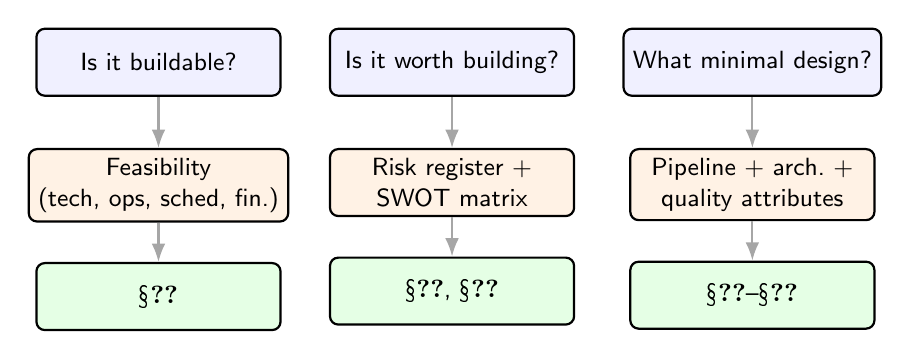
\begin{tikzpicture}[
  font=\sffamily\small,
  node distance=0.5cm and 0.6cm,
  box/.style={draw, rounded corners=3pt, minimum width=3.1cm,
    minimum height=0.85cm, align=center, thick},
  qbox/.style={box, fill=blue!6},
  fbox/.style={box, fill=orange!10},
  abox/.style={box, fill=green!10},
  arrow/.style={-Latex, thick, gray!70},
]
  \node[qbox] (q1) {Is it buildable?};
  \node[qbox, right=of q1] (q2) {Is it worth building?};
  \node[qbox, right=of q2] (q3) {What minimal design?};

  \node[fbox, below=0.65cm of q1] (f1) {Feasibility\\(tech, ops, sched, fin.)};
  \node[fbox, below=0.65cm of q2] (f2) {Risk register + \\ SWOT matrix};
  \node[fbox, below=0.65cm of q3] (f3) {Pipeline + arch.\ + \\ quality attributes};

  \node[abox, below=0.5cm of f1] (a1) {\S\ref{sec:fw-feas}};
  \node[abox, below=0.5cm of f2] (a2) {\S\ref{sec:fw-risk}, \S\ref{sec:fw-swot}};
  \node[abox, below=0.5cm of f3] (a3) {\S\ref{sec:fw-framework}--\S\ref{sec:fw-quality}};

  \foreach \x/\y in {q1/f1, q2/f2, q3/f3, f1/a1, f2/a2, f3/a3} \draw[arrow] (\x) -- (\y);
\end{tikzpicture}}
\caption[Chapter 3 roadmap]{\textbf{Chapter 3 roadmap.} The
chapter answers three gating questions, each answered by a
corresponding analytical artifact, delivered in a specific
downstream section.}
\label{fig:ch3-roadmap}
\end{figure}

\section{Pre-Project Phase -- Feasibility Analysis}
\label{sec:fw-feas}

A feasibility study answers whether a proposed system
\emph{can} and \emph{should} be built given concrete
resource, time, operational, and regulatory constraints
\citep{whitten2007sysanalysis, pressman2015software}. For a
student-led research project the analysis is deliberately
scoped to the four dimensions below; a classical
\emph{Operational} and a classical \emph{Legal} study are
folded into the operational dimension because the project
produces a research artifact rather than a clinical device
(Chapter~\ref{ch:intro}, Section~\ref{sec:intro-scope}).

\subsection{Technical Feasibility}
\label{sec:feas-tech}

Technical feasibility asks whether the proposed pipeline can
be implemented, tested, and maintained on the hardware and
software resources actually available to the team. Our
answer is a confident \emph{yes}. Table~\ref{tab:tech-stack}
lists the exact components in the four architectural layers
of the solution, and Figure~\ref{fig:tech-stack} depicts the
same layering graphically together with the cross-cutting
quality tooling that supports every layer.

\begin{table}[htbp]
\centering
\footnotesize
\begin{tabularx}{\linewidth}{@{}l l X@{}}
\toprule
\textbf{Layer} & \textbf{Component} & \textbf{Role in the pipeline} \\
\midrule
Data &
\textsc{ClinVar} (NCBI) &
labelled catalogue of pathogenic/benign variants with review-star confidence. \\
Data &
\textsc{gnomAD} v2.1 + v4.0 &
population allele frequency and gene-level constraint metrics (pLI, LOEUF). \\
Data &
\textsc{dbNSFP} v4.5 &
pre-computed conservation scores (phyloP, phastCons, GERP++) and amino-acid features. \\
Data &
\textsc{denovo-db} &
external, patient-derived de novo variants for held-out validation. \\
Data &
UniProt / Ensembl VEP &
canonical protein sequences and transcript-aware annotation. \\
\midrule
Language &
Python 3.11 &
main implementation language; chosen for scientific-stack maturity. \\
ML core &
\texttt{xgboost}~2.0 &
gradient-boosted trees; baseline classifier. \\
ML core &
\texttt{scikit-learn}~1.4 &
isotonic / Platt calibration, metric utilities, bootstrap. \\
ML core &
\texttt{optuna}~3.5 &
TPE hyperparameter search with Median Pruner. \\
ML core &
\texttt{shap}~0.44 &
TreeSHAP interpretability. \\
ML core &
\texttt{transformers}~4.41 + \texttt{torch}~2.2 &
ESM-2 zero-shot LLR scoring. \\
\midrule
Interface &
Streamlit~1.33 &
interactive single-variant web application. \\
Interface &
Typer CLI &
batch-mode command-line interface. \\
Interface &
Python package &
programmatic API for downstream integrations. \\
\midrule
Quality &
GitHub Actions CI &
enforces lint, type, and leakage tests on every push. \\
Quality &
Docker + \texttt{uv} lock &
reproducible environment; \texttt{docker run} is sufficient to re-score. \\
Quality &
\texttt{pytest} + \texttt{hypothesis} &
deterministic + property-based tests for the feature pipeline. \\
\bottomrule
\end{tabularx}
\caption[Technology stack]{\textbf{Technology stack.} Every
major component is open-source and pinned in
\texttt{requirements-lock.txt}. The quality row crosses all
other layers.}
\label{tab:tech-stack}
\end{table}

\begin{figure}[htbp]
\centering
\resizebox{\linewidth}{!}{%
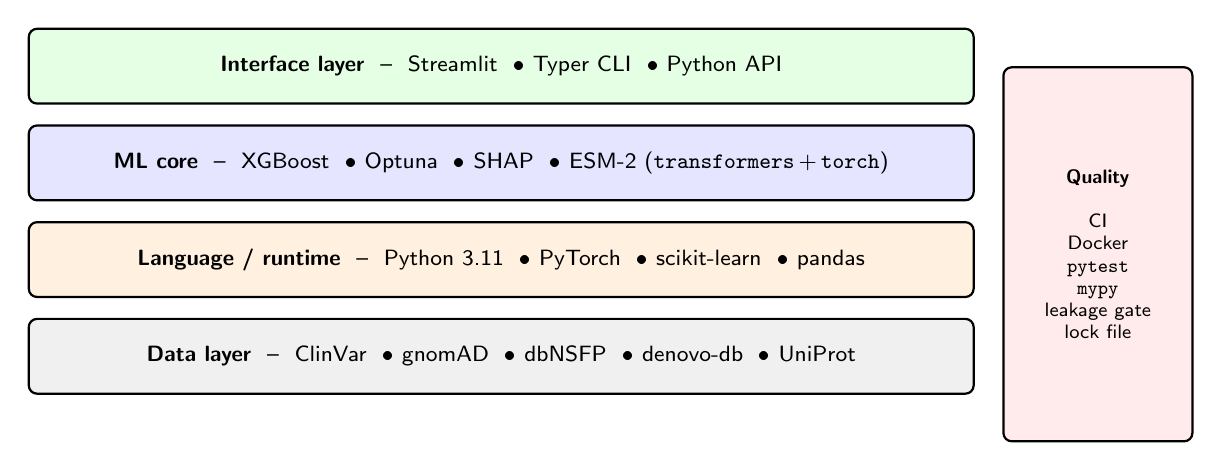
\begin{tikzpicture}[
  font=\sffamily\footnotesize,
  layer/.style={draw, rounded corners=3pt, minimum width=12cm,
    minimum height=0.95cm, align=center, thick},
  qc/.style={draw, rounded corners=3pt, minimum width=2.4cm,
    minimum height=3.6cm, align=center, fill=red!8, thick,
    font=\sffamily\scriptsize},
]
  \node[layer, fill=green!10]  (ui)   {\textbf{Interface layer} \ -- \ Streamlit \ \textbullet\ Typer CLI \ \textbullet\ Python API};
  \node[layer, fill=blue!10,  below=0.25cm of ui]    (ml)   {\textbf{ML core}  \ -- \ XGBoost \ \textbullet\ Optuna \ \textbullet\ SHAP \ \textbullet\ ESM-2 (\texttt{transformers}\,+\,\texttt{torch})};
  \node[layer, fill=orange!12, below=0.25cm of ml]   (lang) {\textbf{Language / runtime} \ -- \ Python 3.11 \ \textbullet\ PyTorch \ \textbullet\ scikit-learn \ \textbullet\ pandas};
  \node[layer, fill=black!6,   below=0.25cm of lang] (data) {\textbf{Data layer} \ -- \ ClinVar \ \textbullet\ gnomAD \ \textbullet\ dbNSFP \ \textbullet\ denovo-db \ \textbullet\ UniProt};
  \node[qc, right=0.35cm of ui.east, anchor=north west, yshift=-0.0cm,
        minimum height=4.75cm]                       (qc)   {\textbf{Quality} \\ \ \\ CI \\ Docker \\ \texttt{pytest} \\ \texttt{mypy} \\ leakage gate \\ lock file};
\end{tikzpicture}}
\caption[Technology-stack diagram]{\textbf{Technology-stack
diagram.} Four horizontal layers plus a vertical quality
band. The quality band is not a layer but a cross-cutting
concern: every commit triggers the same gate chain
regardless of which layer is being modified.}
\label{fig:tech-stack}
\end{figure}

\textbf{Compute budget and wall-clock times.} Every stage in
Part~1 and Part~2 of the pipeline
(Section~\ref{sec:fw-framework}) completes on a consumer
laptop (eight CPU cores, 16~GB RAM) within the time budget
summarised in Table~\ref{tab:compute-budget}. Only two
stages require a GPU: the full-dataset ESM-2 scoring
(offloaded to free Google Colab T4) and the AlphaFold-2
structural feature extraction (likewise Colab T4, CPU-only
fallback available for reproducibility). No paid compute,
no institutional HPC cluster, and no licensed database were
required at any point in the project.

\begin{table}[htbp]
\centering
\footnotesize
\begin{tabularx}{\linewidth}{@{}l l r X@{}}
\toprule
\textbf{Stage} & \textbf{Hardware} & \textbf{Wall-clock} & \textbf{Reason for budget} \\
\midrule
ClinVar + gnomAD + dbNSFP merge &
Laptop CPU &
$\sim$8~min &
Four sequential \texttt{pyarrow} joins on 283k rows. \\
Paralog split + feature engineering &
Laptop CPU &
$\sim$2~min &
Regex classification over $\sim$16k gene symbols. \\
XGBoost training &
Laptop CPU &
$\sim$8~min &
$n=195$k rows, 39 features, 500 trees. \\
Optuna HPO (40 trials) &
Laptop CPU &
$\sim$30~min &
TPE with Median Pruner early-stopping. \\
SHAP on 2k-variant sample &
Laptop CPU &
$\sim$3~min &
TreeSHAP exact algorithm for tree ensembles. \\
ESM-2 35M scoring (denovo-db) &
Colab T4 &
$\sim$45~min &
2{,}000 variants $\times$ 1 forward pass $\times$ 20 amino acids. \\
ESM-2 35M scoring (full train) &
Colab T4 &
$\sim$8~h &
195k unique variants; chunked and resumable. \\
Full thesis + defense compile &
Laptop CPU &
$<$1~min &
\texttt{tectonic} single-pass + bibliography. \\
\bottomrule
\end{tabularx}
\caption[Compute budget]{\textbf{Compute budget.} Every
stage fits inside a free-tier allocation of either a
consumer laptop or a Google Colab T4 session.}
\label{tab:compute-budget}
\end{table}

\subsection{Operational Feasibility}
\label{sec:feas-op}

Operational feasibility asks whether the system, once built,
will actually be used by its intended stakeholders and
whether it produces output that is actionable within their
workflow. Table~\ref{tab:stakeholders} lists the four
stakeholder groups we identified, the concrete need each
group brings to the system, the operational surface we
provide for them, and the decision the system supports.

\begin{table}[htbp]
\centering
\footnotesize
\begin{tabularx}{\linewidth}{@{}l X X X@{}}
\toprule
\textbf{Stakeholder} & \textbf{Need} & \textbf{Surface} & \textbf{Decision supported} \\
\midrule
Clinical geneticist &
calibrated score and per-feature reason for a single variant &
Streamlit web app &
ACMG-adjacent evidence gathering (not replacement). \\
Research scientist &
batch score for a cohort of $\sim$10$^4$--10$^5$ variants &
Typer CLI &
ranked shortlist for follow-up functional assay. \\
Bioinformatics engineer &
programmatic integration into an existing pipeline &
Python package &
variant annotation in a larger analytical workflow. \\
Project examiner &
reproducible artifact with audit trail &
GitHub + Docker image &
verification of the end-to-end claims made in this thesis. \\
\bottomrule
\end{tabularx}
\caption[Stakeholder-to-surface mapping]{\textbf{Stakeholder-to-surface
mapping.} Each operational surface is optimised for one
decision context; no stakeholder is required to retrain the
model or to understand its internals.}
\label{tab:stakeholders}
\end{table}

\textbf{Regulatory scope (important caveat).} The system is
explicitly positioned as a \emph{research} artifact, not as
a diagnostic device. The Saudi Food and Drug Authority
(SFDA) classifies any software that directly drives a
clinical decision as a medical device requiring a separate
and lengthy certification process that is outside the scope
of an undergraduate graduation project. We therefore
constrain every operational surface to emit an advisory
score accompanied by a feature-level justification. A human
expert remains in the decision loop at all times.

\subsection{Schedule Feasibility}
\label{sec:feas-sched}

The project occupied two consecutive academic semesters
(Term~1 -- Fall 2025 and Term~2 -- Spring 2026) at King
Khalid University. Term~1 was dedicated to literature
review, scope lock-down, data ingestion, and a first
XGBoost proof-of-concept. Term~2 was the execution phase:
leakage audit, hyperparameter tuning, calibration, SHAP
analysis, external validation, the ESM-2 proof-of-concept,
and the final academic write-up. Figure~\ref{fig:gantt}
renders the schedule as a TikZ Gantt chart with milestones
marked explicitly for every gating deadline.

\begin{figure}[htbp]
\centering
\resizebox{\linewidth}{!}{%
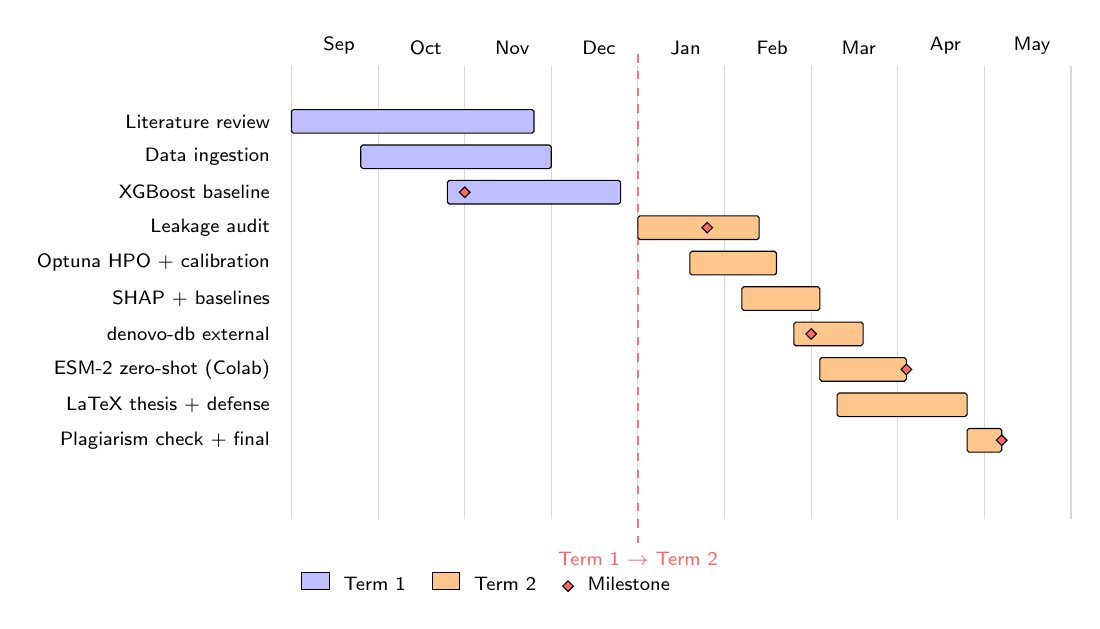
\begin{tikzpicture}[
  font=\sffamily\scriptsize,
  scale=1.0,
  month/.style={font=\sffamily\scriptsize, anchor=south},
  lab/.style={font=\sffamily\scriptsize, anchor=east},
  mile/.style={diamond, draw, fill=red!60, minimum size=4pt, inner sep=0pt},
]
  % Grid: 9 month columns (x=0..9), rows for 10 tasks
  % 1 horizontal unit = 1 month = 1.1 cm
  \def\xu{1.1}

  % Vertical grid lines + month labels
  \foreach \x/\m in {0/Sep, 1/Oct, 2/Nov, 3/Dec, 4/Jan, 5/Feb, 6/Mar, 7/Apr, 8/May, 9/{}} {
    \draw[gray!30] (\x*\xu, 0.25) -- (\x*\xu, -5.5);
    \ifx\m\empty\else\node[month] at (\x*\xu+0.55*\xu, 0.28) {\m};\fi
  }

  % Term 1 / Term 2 separator
  \draw[red!55, dashed, thick] (4*\xu, 0.4) -- (4*\xu, -5.8);
  \node[red!60, font=\sffamily\scriptsize, anchor=north] at (4*\xu, -5.8) {Term 1 $\to$ Term 2};

  % Tasks (start month, end month, row, colour)
  \foreach \s/\e/\r/\c in {%
    0/2.8/1/blue!25,%
    0.8/3.0/2/blue!25,%
    1.8/3.8/3/blue!25,%
    4.0/5.4/4/orange!45,%
    4.6/5.6/5/orange!45,%
    5.2/6.1/6/orange!45,%
    5.8/6.6/7/orange!45,%
    6.1/7.1/8/orange!45,%
    6.3/7.8/9/orange!45,%
    7.8/8.2/10/orange!45%
  }{
    \fill[\c, draw=black, thin, rounded corners=0.7pt]
      (\s*\xu, -\r*0.45+0.15) rectangle (\e*\xu, -\r*0.45-0.15);
  }

  % Task labels (left of chart, inside margin)
  \foreach \r/\t in {%
    1/{Literature review},%
    2/{Data ingestion},%
    3/{XGBoost baseline},%
    4/{Leakage audit},%
    5/{Optuna HPO + calibration},%
    6/{SHAP + baselines},%
    7/{denovo-db external},%
    8/{ESM-2 zero-shot (Colab)},%
    9/{LaTeX thesis + defense},%
    10/{Plagiarism check + final}%
  }{
    \node[lab] at (-0.15, -\r*0.45) {\t};
  }

  % Milestones (red diamonds)
  \foreach \x/\r in {2.0/3, 4.8/4, 6.0/7, 7.1/8, 8.2/10}
    \node[mile] at (\x*\xu, -\r*0.45) {};

  % Legend below
  \node[font=\sffamily\scriptsize, anchor=west] at (0, -6.3)
    {\tikz{\fill[blue!25, draw=black, thin] (0,0) rectangle (0.35,0.22);} \ Term 1
     \hspace{0.6em}
     \tikz{\fill[orange!45, draw=black, thin] (0,0) rectangle (0.35,0.22);} \ Term 2
     \hspace{0.6em}
     \tikz[baseline=-0.5ex]{\node[mile]{};} \ Milestone};
\end{tikzpicture}}
\caption[Two-semester Gantt chart]{\textbf{Two-semester Gantt
chart.} Term 1 (blue) covered literature review, data
ingestion, and the first XGBoost baseline. Term 2 (orange)
covered the leakage audit, hyperparameter search,
calibration, SHAP, external validation, ESM-2 scoring, and
the academic write-up. Red diamonds mark unambiguous
quantitative milestones.}
\label{fig:gantt}
\end{figure}

Two organisational rules were applied to keep the schedule
on track. First, the leakage audit, calibration, and SHAP
work were treated as \emph{blocking} for any further
experimentation; the quantitative claims of the thesis all
flow from a single audited checkpoint. Second, the LaTeX
write-up and the ESM-2 training-set scoring were scheduled
in parallel so that the academic deliverable did not block
on a GPU-bound experiment that depended on Colab availability.

\subsection{Financial Feasibility}
\label{sec:feas-fin}

The direct financial cost of the project is zero. No
licensed databases, no commercial GPU rental, and no paid
software subscriptions were used at any point.
Table~\ref{tab:tco} compares the project's realised
zero-cost profile against a hypothetical commercial
counterfactual, computing the implicit cost avoidance.

\begin{table}[htbp]
\centering
\footnotesize
\begin{tabularx}{\linewidth}{@{}X r r l@{}}
\toprule
\textbf{Item} & \textbf{Commercial cost (USD)} & \textbf{Our cost} & \textbf{Replacement strategy} \\
\midrule
HGMD Pro annual licence &
$\sim$5{,}000 &
0 &
ClinVar (expert-reviewed) only. \\
AWS p3.2xlarge 8h (V100) for ESM-2 &
$\sim$25 &
0 &
Free Colab T4 with chunked resume. \\
AlphaFold-3 API monthly &
$\sim$200 &
0 &
AlphaFold-2 Colab + local cache. \\
Enterprise issue tracker + CI &
$\sim$40 / mo &
0 &
GitHub Actions free tier. \\
\midrule
\textbf{Total avoidance (8 months)} &
\textbf{$\sim$5{,}545} &
\textbf{0} & \\
\bottomrule
\end{tabularx}
\caption[Cost avoidance]{\textbf{Cost avoidance.} Every
commercially-priced building block has a zero-cost
open-source or academic-tier replacement.}
\label{tab:tco}
\end{table}

The indirect cost is approximately eight person-months of
student labour distributed across six team members plus ten
supervisory hours per month from the project supervisor; no
direct monetary equivalent is assigned because the project
is academic and no external sponsor is involved.

\section{Risk Analysis}
\label{sec:fw-risk}

A formal risk register was maintained throughout the project
(mirrored in \texttt{docs/CHANGELOG.md}). Each risk was
rated on a $5\times 5$ likelihood $\times$ impact grid
\citep{hillson2002risk}, with mitigation actions that were
either preventive (applied before the risk could occur) or
corrective (applied after detection). Table~\ref{tab:risks}
lists the eight most material risks; Figure~\ref{fig:risk-matrix}
renders the same risks on the $5\times 5$ heat-map that the
project team used in supervision meetings.

\begin{table}[htbp]
\centering
\footnotesize
\begin{tabularx}{\linewidth}{@{}l X c c X@{}}
\toprule
\textbf{ID} & \textbf{Risk} & \textbf{L} & \textbf{I} & \textbf{Mitigation} \\
\midrule
R1 & Paralog leakage inflates AUROC          & 5 & 5 & \emph{Preventive:} paralog-aware \texttt{GroupShuffleSplit} + CI-enforced leakage gate. \\
R2 & Meta-predictor circular evaluation      & 5 & 5 & \emph{Preventive:} banned-feature list; AlphaMissense re-scored, never used as feature. \\
R3 & ClinVar label instability across versions & 3 & 4 & \emph{Corrective:} pin 2024-01 release; record version in \texttt{CHANGELOG.md}. \\
R4 & Colab GPU quota exhaustion during ESM-2 & 4 & 3 & \emph{Corrective:} checkpointed chunked scoring; resumable from arbitrary offset. \\
R5 & PLM scoring non-determinism (GPU kernels) & 3 & 2 & \emph{Corrective:} fix seed; eval-mode; single-token LLR is deterministic to 6~dp. \\
R6 & Calibration drift after feature change & 4 & 3 & \emph{Preventive:} isotonic refit is part of CI; Brier re-measured on every push. \\
R7 & Late-semester scope creep (CNN-BiLSTM)   & 5 & 4 & \emph{Preventive:} scope lock at mid-Term 2 (see \ref{sec:intro-scope}); deferred to future work. \\
R8 & LaTeX build fails in the defence week   & 4 & 4 & \emph{Preventive:} \texttt{tectonic} single-pass + locked fonts; CI builds the PDF. \\
\bottomrule
\end{tabularx}
\caption[Risk register]{\textbf{Risk register.} L =
likelihood (1--5), I = impact (1--5). A risk's score is the
product $L\times I$; any risk with a score $\geq 12$
required a documented mitigation before work could proceed.}
\label{tab:risks}
\end{table}

\begin{figure}[htbp]
\centering
\resizebox{\linewidth}{!}{%
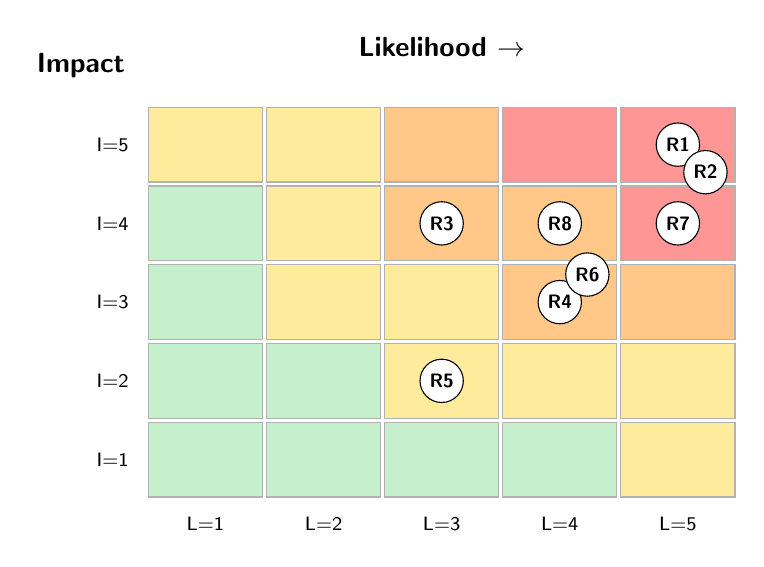
\begin{tikzpicture}[
  font=\sffamily\footnotesize,
  cell/.style={draw=gray!60, minimum width=1.45cm, minimum height=0.95cm, inner sep=0pt},
  rlabel/.style={font=\sffamily\scriptsize, anchor=east},
  clabel/.style={font=\sffamily\scriptsize, anchor=north},
  risk/.style={circle, draw=black, fill=white, inner sep=1pt,
    font=\sffamily\bfseries\scriptsize, minimum size=0.55cm},
]
  % Colour gradient: L*I < 5 green, 5-11 yellow, 12-19 orange, 20-25 red
  \foreach \col/\L in {1/1, 2/2, 3/3, 4/4, 5/5}{
    \foreach \row/\I in {1/1, 2/2, 3/3, 4/4, 5/5}{
      \pgfmathsetmacro{\score}{\L*\I}
      \ifdim \score pt < 5pt
        \definecolor{cc}{RGB}{198,239,206}%
      \else
        \ifdim \score pt < 12pt
          \definecolor{cc}{RGB}{255,235,156}%
        \else
          \ifdim \score pt < 20pt
            \definecolor{cc}{RGB}{255,199,136}%
          \else
            \definecolor{cc}{RGB}{255,150,150}%
          \fi
        \fi
      \fi
      \node[cell, fill=cc] at (\col*1.5, \row*1) {};
    }
  }

  % Axis labels
  \foreach \col/\L in {1/1, 2/2, 3/3, 4/4, 5/5} \node[clabel] at (\col*1.5, 0.4) {L=\L};
  \foreach \row/\I in {1/1, 2/2, 3/3, 4/4, 5/5} \node[rlabel] at (0.65, \row*1) {I=\I};

  \node[font=\sffamily\bfseries, anchor=east] at (0.6, 6) {Impact};
  \node[font=\sffamily\bfseries, anchor=south] at (4.5, 6) {Likelihood $\to$};

  % Plot risks
  \node[risk] at (5*1.5, 5*1)   {R1};
  \node[risk] at (5*1.5+0.35, 5*1-0.35) {R2};
  \node[risk] at (3*1.5, 4*1)   {R3};
  \node[risk] at (4*1.5, 3*1)   {R4};
  \node[risk] at (3*1.5, 2*1)   {R5};
  \node[risk] at (4*1.5+0.35, 3*1+0.35) {R6};
  \node[risk] at (5*1.5, 4*1)   {R7};
  \node[risk] at (4*1.5, 4*1)   {R8};
\end{tikzpicture}}
\caption[Risk matrix]{\textbf{Risk matrix.} Cells shaded by
$L\times I$ score: green $<5$, yellow $5$--$11$, orange
$12$--$19$, red $\geq 20$. Every red-cell risk (R1, R2, R7)
triggered a preventive mitigation before implementation
began; yellow and orange risks received corrective
mitigations documented in \texttt{CHANGELOG.md}.}
\label{fig:risk-matrix}
\end{figure}

\section{SWOT Analysis}
\label{sec:fw-swot}

A strengths-weaknesses-opportunities-threats (SWOT) matrix
\citep{humphrey2005swot} summarises the project's competitive
position relative to the prior work reviewed in
Chapter~\ref{ch:related}. Figure~\ref{fig:swot} renders the
four quadrants; each item is a concrete statement traceable
to a specific section of this thesis.

\begin{figure}[htbp]
\centering
\resizebox{\linewidth}{!}{%
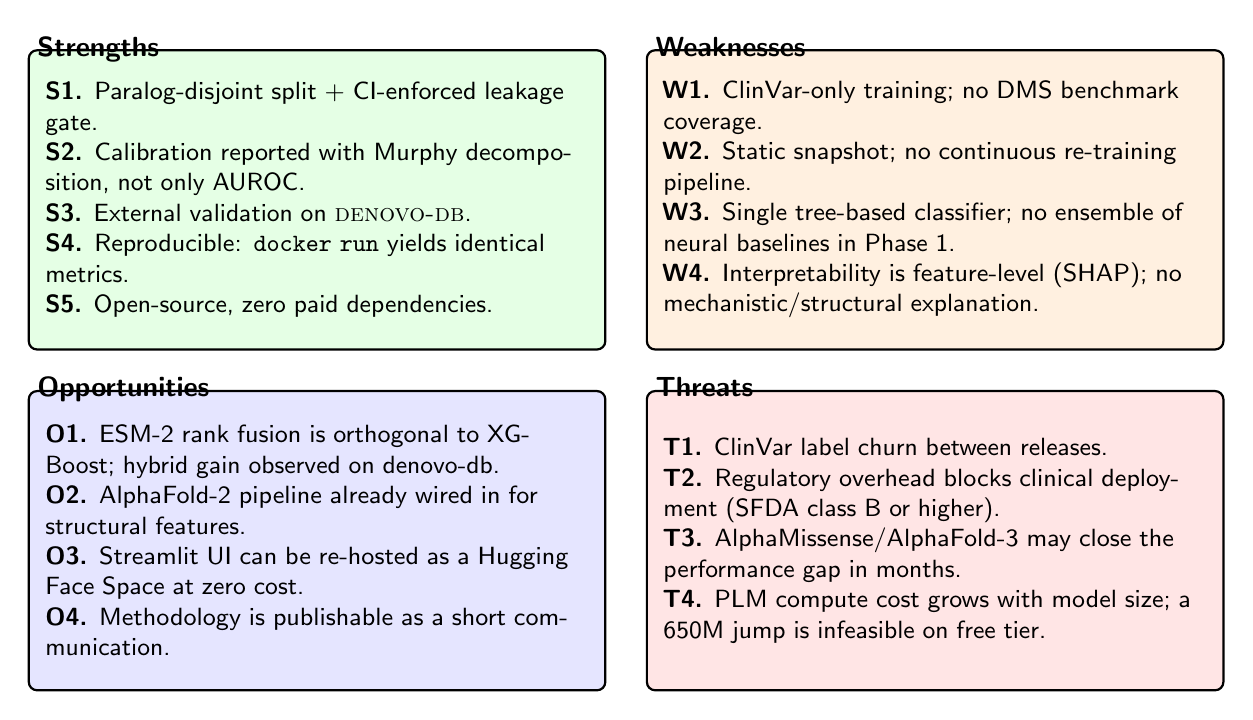
\begin{tikzpicture}[
  font=\sffamily\footnotesize,
  quad/.style={draw, rounded corners=3pt, minimum width=7.3cm,
    minimum height=3.8cm, align=left, inner sep=6pt, thick,
    text width=6.9cm},
  title/.style={font=\sffamily\bfseries, anchor=north west, yshift=0.28cm},
]
  \node[quad, fill=green!10] (S) at (0, 0)
    {\begin{minipage}{6.7cm}\small
     \textbf{S1.} Paralog-disjoint split $+$ CI-enforced leakage gate.\\
     \textbf{S2.} Calibration reported with Murphy decomposition, not only AUROC.\\
     \textbf{S3.} External validation on \textsc{denovo-db}.\\
     \textbf{S4.} Reproducible: \texttt{docker run} yields identical metrics.\\
     \textbf{S5.} Open-source, zero paid dependencies.
     \end{minipage}};
  \node[title] at (S.north west) {Strengths};

  \node[quad, fill=orange!12, right=0.5cm of S] (W)
    {\begin{minipage}{6.7cm}\small
     \textbf{W1.} ClinVar-only training; no DMS benchmark coverage.\\
     \textbf{W2.} Static snapshot; no continuous re-training pipeline.\\
     \textbf{W3.} Single tree-based classifier; no ensemble of neural baselines in Phase~1.\\
     \textbf{W4.} Interpretability is feature-level (SHAP); no mechanistic/structural explanation.
     \end{minipage}};
  \node[title] at (W.north west) {Weaknesses};

  \node[quad, fill=blue!10, below=0.5cm of S] (O)
    {\begin{minipage}{6.7cm}\small
     \textbf{O1.} ESM-2 rank fusion is orthogonal to XGBoost; hybrid gain observed on denovo-db.\\
     \textbf{O2.} AlphaFold-2 pipeline already wired in for structural features.\\
     \textbf{O3.} Streamlit UI can be re-hosted as a Hugging Face Space at zero cost.\\
     \textbf{O4.} Methodology is publishable as a short communication.
     \end{minipage}};
  \node[title] at (O.north west) {Opportunities};

  \node[quad, fill=red!10, right=0.5cm of O] (T)
    {\begin{minipage}{6.7cm}\small
     \textbf{T1.} ClinVar label churn between releases.\\
     \textbf{T2.} Regulatory overhead blocks clinical deployment (SFDA class B or higher).\\
     \textbf{T3.} AlphaMissense/AlphaFold-3 may close the performance gap in months.\\
     \textbf{T4.} PLM compute cost grows with model size; a 650M jump is infeasible on free tier.
     \end{minipage}};
  \node[title] at (T.north west) {Threats};
\end{tikzpicture}}
\caption[SWOT matrix]{\textbf{SWOT matrix} relative to the
prior work reviewed in Chapter~\ref{ch:related}. Strengths
and weaknesses are internal; opportunities and threats are
external.}
\label{fig:swot}
\end{figure}

\section{Proposed Framework -- Three-Part Pipeline}
\label{sec:fw-framework}

The project pipeline decomposes into three sequential parts,
each with a distinct scientific role, a single public
output artifact, and an explicit contract with the next
part. Figure~\ref{fig:pipeline} renders the pipeline as a
swim-lane TikZ diagram; the three rows correspond to the
three parts and the arrows carry the artifact names.

\begin{figure}[htbp]
\centering
\resizebox{\linewidth}{!}{%
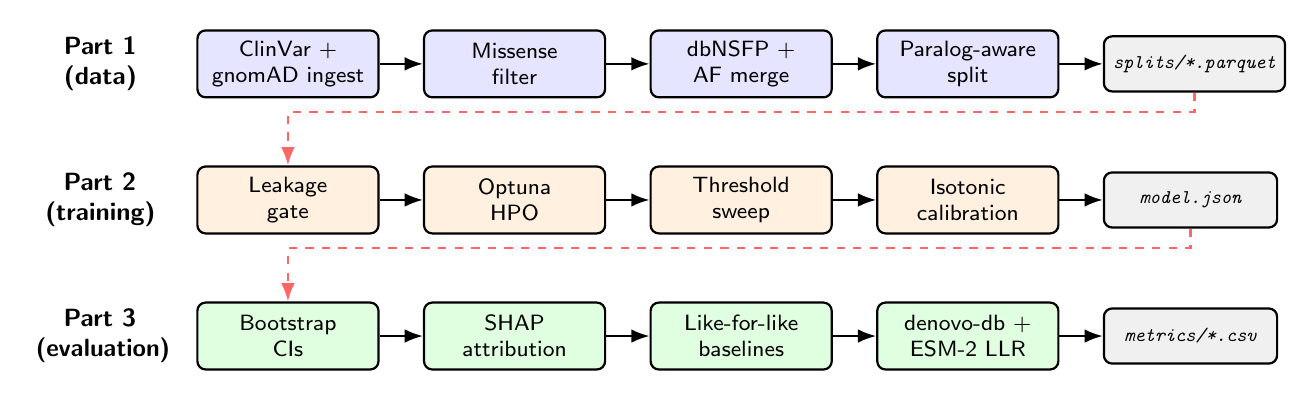
\begin{tikzpicture}[
  font=\sffamily\footnotesize,
  node distance=0.4cm and 0.55cm,
  stage/.style={draw, rounded corners=3pt, minimum width=2.3cm,
    minimum height=0.85cm, align=center, thick},
  part1/.style={stage, fill=blue!10},
  part2/.style={stage, fill=orange!12},
  part3/.style={stage, fill=green!12},
  artf/.style={draw, rounded corners=3pt, minimum width=2.2cm,
    minimum height=0.7cm, align=center, fill=black!6, thick,
    font=\sffamily\scriptsize\itshape},
  arrow/.style={-Latex, thick},
  lane/.style={font=\sffamily\bfseries\small, align=center, text width=1.6cm},
]
  % Part 1
  \node[part1] (ing)   {ClinVar +\\gnomAD ingest};
  \node[part1, right=of ing] (miss)  {Missense\\filter};
  \node[part1, right=of miss] (feat) {dbNSFP +\\AF merge};
  \node[part1, right=of feat] (para) {Paralog-aware\\split};
  \node[artf, right=of para] (art1) {\texttt{splits/*.parquet}};
  \node[lane, left=0.3cm of ing] (ln1) {Part 1\\(data)};

  % Part 2
  \node[part2, below=0.85cm of ing] (gate)  {Leakage\\gate};
  \node[part2, right=of gate] (opt)  {Optuna\\HPO};
  \node[part2, right=of opt] (thr)   {Threshold\\sweep};
  \node[part2, right=of thr] (cal)   {Isotonic\\calibration};
  \node[artf, right=of cal] (art2)    {\texttt{model.json}};
  \node[lane, left=0.3cm of gate] (ln2) {Part 2\\(training)};

  % Part 3
  \node[part3, below=0.85cm of gate] (boot) {Bootstrap\\CIs};
  \node[part3, right=of boot] (shap) {SHAP\\attribution};
  \node[part3, right=of shap] (base) {Like-for-like\\baselines};
  \node[part3, right=of base] (ext)  {denovo-db +\\ESM-2 LLR};
  \node[artf, right=of ext]  (art3)   {\texttt{metrics/*.csv}};
  \node[lane, left=0.3cm of boot] (ln3) {Part 3\\(evaluation)};

  % Arrows within part
  \foreach \a/\b in {ing/miss, miss/feat, feat/para, para/art1,
                     gate/opt, opt/thr, thr/cal, cal/art2,
                     boot/shap, shap/base, base/ext, ext/art3}
    \draw[arrow] (\a) -- (\b);

  % Between-parts artifact flow
  \draw[arrow, dashed, red!60] (art1.south) -- ++(0,-0.25) -| (gate.north);
  \draw[arrow, dashed, red!60] (art2.south) -- ++(0,-0.25) -| (boot.north);
\end{tikzpicture}}
\caption[Three-part pipeline]{\textbf{Three-part pipeline.}
Each row is a \emph{part} with its own responsibility and
output artifact. Solid arrows carry intermediate data
between stages; dashed red arrows are cross-part contracts
-- Part~1's parquet splits feed Part~2, Part~2's
\texttt{model.json} feeds Part~3.}
\label{fig:pipeline}
\end{figure}

\subsection{Part 1 -- Data Preprocessing}
\label{sec:fw-part1}

Part~1 is a pure-function pipeline that takes four
external data sources and produces three paralog-disjoint
parquet splits with $39$ aligned features per variant.
The final feature vector decomposes into five semantically
meaningful groups that together cover sequence
conservation, biochemistry, population genetics, and
gene-level constraint (Figure~\ref{fig:feature-groups}).
This grouping structure is the natural unit of analysis
for the SHAP interpretation of Section~\ref{sec:res-shap}.

\begin{figure}[htbp]
\centering
\resizebox{\linewidth}{!}{%
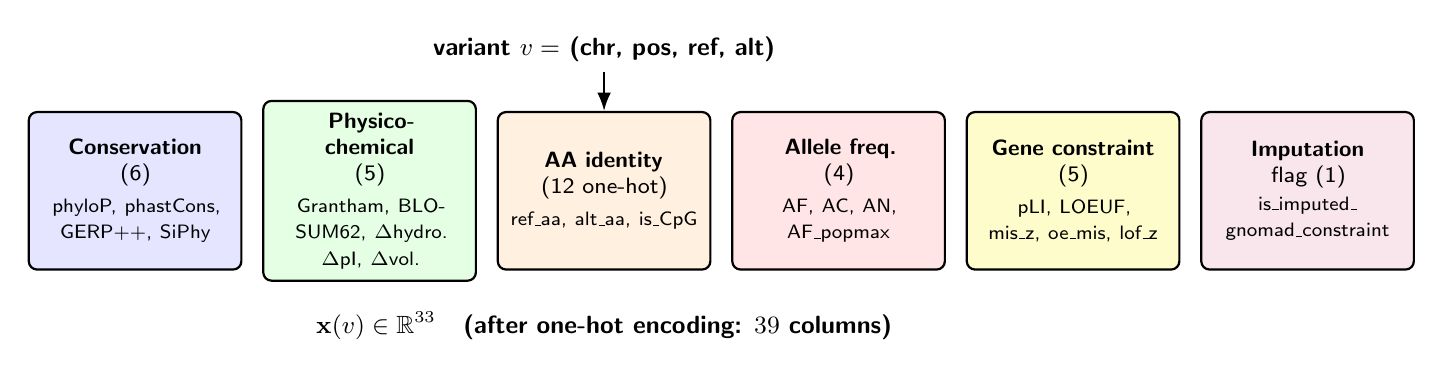
\begin{tikzpicture}[
  font=\sffamily\footnotesize,
  grp/.style={draw, rounded corners=3pt, minimum height=2.0cm,
    thick, align=center, text width=2.4cm, inner sep=0.15cm},
  cons/.style={grp, fill=blue!10},
  phys/.style={grp, fill=green!10},
  aa/.style={grp, fill=orange!12},
  af/.style={grp, fill=red!10},
  struct/.style={grp, fill=purple!10},
  gene/.style={grp, fill=yellow!20},
]
  \node[cons]   (c) at (0, 0)    {\textbf{Conservation}\\(6)\\[2pt]\scriptsize phyloP, phastCons, GERP++, SiPhy};
  \node[phys, right=0.25cm of c] (p) {\textbf{Physico-\\chemical}\\(5)\\[2pt]\scriptsize Grantham, BLOSUM62, $\Delta$hydro.\, $\Delta$pI, $\Delta$vol.};
  \node[aa, right=0.25cm of p]   (a) {\textbf{AA identity}\\(12 one-hot)\\[2pt]\scriptsize ref\_aa, alt\_aa, is\_CpG};
  \node[af, right=0.25cm of a]   (f) {\textbf{Allele freq.}\\(4)\\[2pt]\scriptsize AF, AC, AN, AF\_popmax};
  \node[gene, right=0.25cm of f] (g) {\textbf{Gene constraint}\\(5)\\[2pt]\scriptsize pLI, LOEUF, mis\_z, oe\_mis, lof\_z};
  \node[struct, right=0.25cm of g] (s) {\textbf{Imputation}\\flag (1)\\[2pt]\scriptsize is\_imputed\_\\gnomad\_constraint};

  % Input / output
  \node[font=\sffamily\small\bfseries, above=0.5cm of a] (in)
    {variant $v = $ (chr, pos, ref, alt)};
  \node[font=\sffamily\small\bfseries, below=0.4cm of a] (out)
    {$\mathbf{x}(v) \in \mathbb{R}^{33}$ \ \ (after one-hot encoding: $39$ columns)};

  \draw[-Latex, thick] (in) -- (a.north);
\end{tikzpicture}}
\caption[Feature groups]{\textbf{Feature groups.} The 39
feature columns of the training matrix cluster into
six semantic groups: sequence conservation, physicochemical
distance between \texttt{ref\_aa} and \texttt{alt\_aa},
amino-acid identity (one-hot), gnomAD allele frequency,
gene-level constraint, and an imputation flag. The groups
are the natural unit of SHAP aggregation
(Section~\ref{sec:res-shap}).}
\label{fig:feature-groups}
\end{figure}

The steps, in order, are:

\begin{enumerate}
\item \textbf{ClinVar ingestion.} Download
\texttt{variant\_summary.txt.gz} for the January 2024
release and retain only rows with review-star rating of
two or higher (\texttt{reviewed}, \texttt{reviewed-by-expert-panel},
or \texttt{reviewed-by-multiple-submitters}).
\item \textbf{Missense filter.} Drop every row in which
\texttt{ref\_aa} or \texttt{alt\_aa} is null. This is the
single most important cleaning step because of the
leakage it removes (Section~\ref{sec:feas-audit-miss}).
\item \textbf{gnomAD allele-frequency merge.} Join
\textsc{gnomAD} v2.1 (exomes) and v4.0 (genomes) on
\texttt{chr:pos:ref:alt} to supply per-variant allele
frequency, allele number, and allele count.
\item \textbf{dbNSFP conservation and amino-acid merge.}
Join against a cached \textsc{dbNSFP} extraction
providing phyloP, phastCons, GERP++, BLOSUM62, Grantham
distance, and physicochemical properties of the
substitution.
\item \textbf{gnomAD gene-level constraint merge.} Add
\texttt{pLI}, \texttt{LOEUF} (\texttt{oe\_lof\_upper}),
\texttt{mis\_z}, \texttt{oe\_mis\_upper}, and
\texttt{lof\_z} per gene. Median imputation is fit on the
training split only and applied to val/test, with an
\texttt{is\_imputed\_gnomad\_constraint} flag per row.
\item \textbf{Paralog-aware split.} Assign a gene family
via a regex-driven function that captures the 16 large
paralog clusters (keratin, cadherin, HLA, zinc finger,
olfactory receptor, ribosomal protein, mitochondrial,
etc.), then split at the family level using
\texttt{GroupShuffleSplit} with \texttt{seed=42} and a
$70/15/15$ ratio.
\end{enumerate}

\subsection{Part 2 -- Model Training and Leakage Audit}
\label{sec:fw-part2}

Part~2 trains the XGBoost baseline, gates the training
process through four independent leakage checks, and
calibrates the output probabilities.

\begin{enumerate}
\item \textbf{Leakage gate (pre-training).} Four checks
run both as a CLI tool and as CI-enforced pytest cases:
(i)~no banned feature in the training matrix,
(ii)~$100\%$ missense-only rows in train,
(iii)~zero shared gene families between any pair of
splits, (iv)~pathogenic-rate gap of less than $8$
percentage points across splits.
Algorithm~\ref{alg:leakage-gate} states the gate
formally.
\item \textbf{Optuna hyperparameter search.} We use a
Tree-structured Parzen Estimator sampler
\citep{bergstra2011tpe} with $40$ trials, Median Pruner
early-stopping on PR-AUC, and \texttt{scale\_pos\_weight}
set from the class balance. The search loop is
summarised in Algorithm~\ref{alg:tpe}.
\item \textbf{Threshold sweep.} We search thresholds in
$[0.20, 0.80]$ on validation F1, then freeze the best
threshold for test scoring.
\item \textbf{Calibration.} Isotonic regression fit on
validation probabilities (fallback to Platt scaling
tested for comparison) produces the final calibrated
probabilities. The Murphy decomposition
\citep{murphy1973brier} is used to partition Brier
error into reliability, resolution, and uncertainty.
\end{enumerate}

\begin{algorithm}[htbp]
\caption{Four-invariant leakage gate}
\label{alg:leakage-gate}
\begin{algorithmic}[1]
\Require train/val/test feature matrices $X_{\text{tr}}, X_{\text{val}}, X_{\text{te}}$; banned feature set $\mathcal{B}$; gene families per row $g_i$
\State $E \gets \emptyset$ \Comment{error list}
\If{$\text{cols}(X_{\text{tr}}) \cap \mathcal{B} \neq \emptyset$}
  \State $E \gets E \cup \{\text{``banned features present''}\}$
\EndIf
\If{$\exists i \in X_{\text{tr}} : \text{ref\_aa}(i) \text{ is null}$}
  \State $E \gets E \cup \{\text{``non-missense row in train''}\}$
\EndIf
\For{each pair $(S_1, S_2) \in \{\text{tr/val, tr/te, val/te}\}$}
  \If{$\{g_i : i \in S_1\} \cap \{g_j : j \in S_2\} \neq \emptyset$}
    \State $E \gets E \cup \{\text{``paralog family overlap in } S_1/S_2\text{''}\}$
  \EndIf
\EndFor
\For{each split $S \in \{\text{tr, val, te}\}$}
  \State $\pi_S \gets \text{pathogenic rate on } S$
\EndFor
\If{$\max_S \pi_S - \min_S \pi_S > 0.08$}
  \State $E \gets E \cup \{\text{``class-balance drift across splits''}\}$
\EndIf
\State \Return $E$ \Comment{empty $\Rightarrow$ pass; else $\Rightarrow$ halt build}
\end{algorithmic}
\end{algorithm}

\begin{algorithm}[htbp]
\caption{Optuna TPE hyperparameter search}
\label{alg:tpe}
\begin{algorithmic}[1]
\Require search space $\Theta$; train $X_{\text{tr}}, y_{\text{tr}}$; val $X_{\text{val}}, y_{\text{val}}$; $n_{\text{trials}}=40$; seed $s=42$
\State $\rho \gets \tfrac{|\{i : y_i = 0\}|}{|\{i : y_i = 1\}|}$ \Comment{scale\_pos\_weight from class balance}
\State sampler $\gets \textsc{TPESampler}(\text{multivariate}=\text{true}, \text{group}=\text{true}, \text{seed}=s)$
\State pruner $\gets \textsc{MedianPruner}(n_{\text{warmup}}=5, n_{\text{startup}}=10)$
\State create study $\mathcal{S}$ with direction $=$ maximise, sampler, pruner
\For{$t = 1 \ldots n_{\text{trials}}$}
  \State $\theta_t \gets \text{sampler.suggest}(\Theta, \text{history}=\mathcal{S})$
  \State fit booster with $\theta_t$ and $\rho$ on $X_{\text{tr}}, y_{\text{tr}}$
  \State $p_{\text{val}} \gets \text{booster.predict\_proba}(X_{\text{val}})$
  \State $\text{PR-AUC}_t \gets \text{prauc}(y_{\text{val}}, p_{\text{val}})$
  \State \textbf{if} pruner says ``prune'' after intermediate step \textbf{then} abort trial
  \State $\mathcal{S}.\text{record}(\theta_t, \text{PR-AUC}_t)$
\EndFor
\State \Return $\arg\max_{\theta_t} \text{PR-AUC}_t$
\end{algorithmic}
\end{algorithm}

\subsection{Part 3 -- Evaluation, Interpretability, and External Validation}
\label{sec:fw-part3}

Part~3 takes the trained model and runs five parallel
evaluations (Figure~\ref{fig:evalflow}):

\begin{enumerate}
\item \textbf{Bootstrap confidence intervals.} $1{,}000$
non-parametric replicates for ROC-AUC, PR-AUC, F1, MCC,
and Brier loss, following the methodology of
\citet{efron1986bootstrap}.
\item \textbf{TreeSHAP interpretability.} SHAP values
\citep{lundberg2017shap, lundberg2020treeshap} are
computed on a stratified $2{,}000$-variant sample for
per-feature attribution.
\item \textbf{Like-for-like baselines.} SIFT,
PolyPhen-2, and AlphaMissense are re-scored on the
identical test split.
\item \textbf{External validation on \textsc{denovo-db}}
with pre- and post-gnomAD-constraint numbers, and
family-holdout-only slicing.
\item \textbf{ESM-2 zero-shot proof-of-concept.} The
log-likelihood ratio from \texttt{esm2\_t12\_35M\_UR50D}
is computed on \textsc{denovo-db} and fused with the
XGBoost probability at the rank level to test
orthogonality.
\end{enumerate}

\begin{figure}[htbp]
\centering
\resizebox{\linewidth}{!}{%
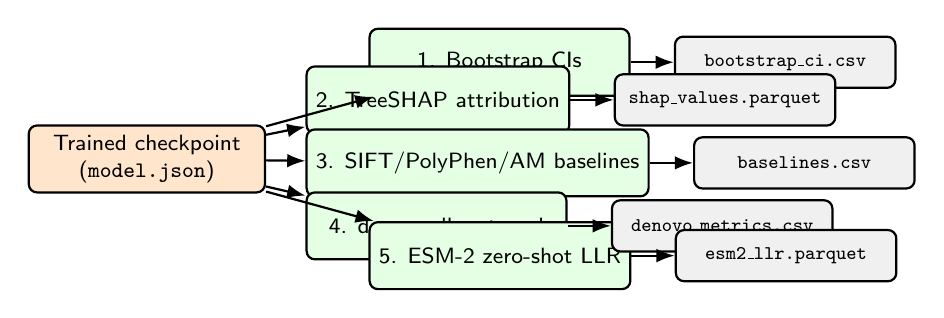
\begin{tikzpicture}[
  font=\sffamily\footnotesize,
  node distance=0.55cm and 0.5cm,
  ckpt/.style={draw, rounded corners=3pt, minimum width=3.0cm,
    minimum height=0.85cm, align=center, fill=orange!20, thick},
  track/.style={draw, rounded corners=3pt, minimum width=3.3cm,
    minimum height=0.85cm, align=center, fill=green!10, thick},
  art/.style={draw, rounded corners=3pt, minimum width=2.8cm,
    minimum height=0.65cm, align=center, fill=black!6,
    font=\sffamily\scriptsize\ttfamily, thick},
  arrow/.style={-Latex, thick},
]
  \node[ckpt] (m) {Trained checkpoint\\(\texttt{model.json})};

  \node[track, above right=0.35cm and 1.3cm of m] (t1) {1. Bootstrap CIs};
  \node[track, right=of m, yshift=0.75cm] (t2) {2. TreeSHAP attribution};
  \node[track, right=of m, yshift=-0.05cm] (t3) {3. SIFT/PolyPhen/AM baselines};
  \node[track, right=of m, yshift=-0.85cm] (t4) {4. denovo-db external};
  \node[track, below right=0.35cm and 1.3cm of m] (t5) {5. ESM-2 zero-shot LLR};

  \node[art, right=0.55cm of t1] (a1) {bootstrap\_ci.csv};
  \node[art, right=0.55cm of t2] (a2) {shap\_values.parquet};
  \node[art, right=0.55cm of t3] (a3) {baselines.csv};
  \node[art, right=0.55cm of t4] (a4) {denovo\_metrics.csv};
  \node[art, right=0.55cm of t5] (a5) {esm2\_llr.parquet};

  \foreach \a/\b in {m/t1, m/t2, m/t3, m/t4, m/t5,
                     t1/a1, t2/a2, t3/a3, t4/a4, t5/a5}
    \draw[arrow] (\a) -- (\b);
\end{tikzpicture}}
\caption[Evaluation workflow]{\textbf{Evaluation workflow.} A
single audited checkpoint feeds five independent evaluation
tracks that run in parallel. Each track writes its own
versioned artifact in \texttt{results/metrics/} so that any
single track can be reproduced without re-running the
others.}
\label{fig:evalflow}
\end{figure}

\section{Proposed System Architecture}
\label{sec:fw-arch}

The logical architecture of the system is a six-layer stack
with two cross-cutting concerns
(Figure~\ref{fig:arch}). Layers are ordered from the
external data sources at the bottom to the user interfaces
at the top, reflecting the flow of a request from the
outside world down to the data and back. Each layer exposes
a narrow interface to the layer above and is explicitly
unaware of the layer below. The \emph{quality gates} concern
(lint, type-check, unit + property tests, leakage gate, CI)
and the \emph{reproducibility} concern (Docker, \texttt{uv}
lock file, fixed seeds, immutable data snapshots) are
attached horizontally because they touch every layer
simultaneously.

\begin{figure}[htbp]
\centering
\resizebox{\linewidth}{!}{%
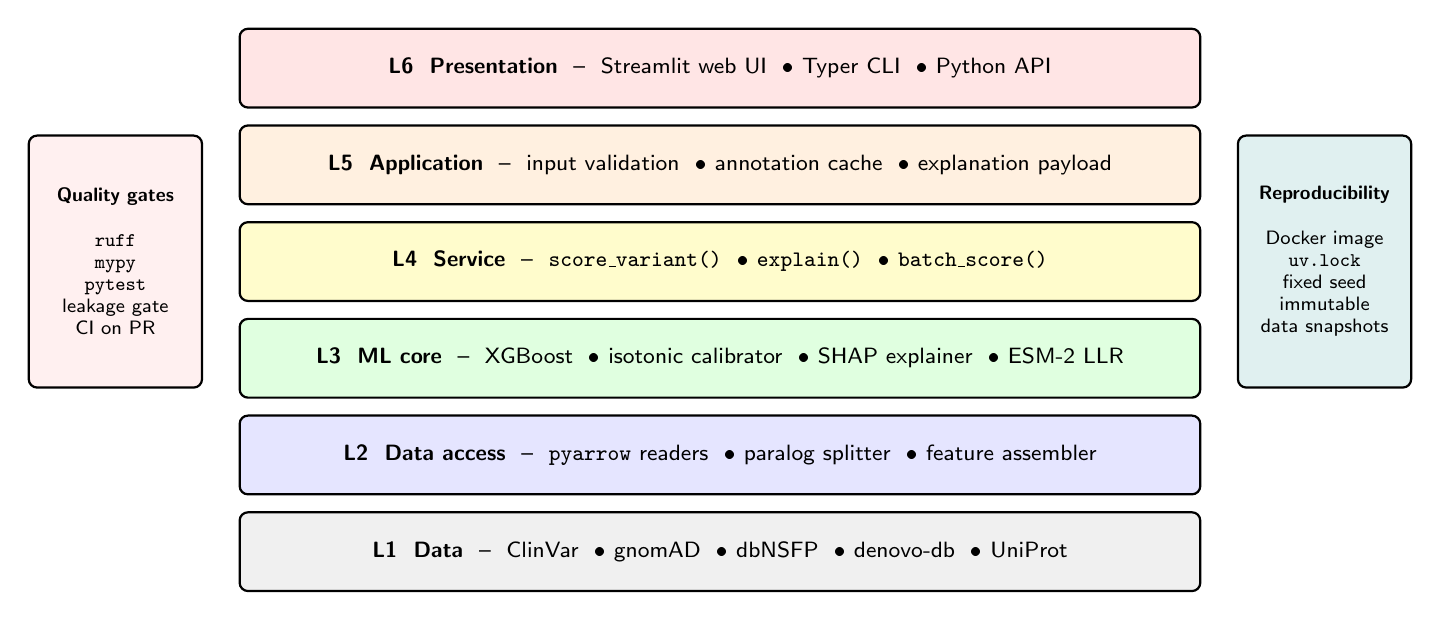
\begin{tikzpicture}[
  font=\sffamily\footnotesize,
  layer/.style={draw, rounded corners=3pt, minimum width=12.2cm,
    minimum height=1.0cm, align=center, thick},
  cross/.style={draw, rounded corners=3pt, minimum width=2.2cm,
    minimum height=3.2cm, align=center, thick, font=\sffamily\scriptsize},
]
  % Top to bottom: presentation -> application -> service -> ML core -> data access -> data
  \node[layer, fill=red!10]    (l6) {\textbf{L6~~Presentation} \ -- \ Streamlit web UI \ \textbullet\ Typer CLI \ \textbullet\ Python API};
  \node[layer, fill=orange!12, below=0.2cm of l6] (l5) {\textbf{L5~~Application} \ -- \ input validation \ \textbullet\ annotation cache \ \textbullet\ explanation payload};
  \node[layer, fill=yellow!20, below=0.2cm of l5] (l4) {\textbf{L4~~Service} \ -- \ \texttt{score\_variant()} \ \textbullet\ \texttt{explain()} \ \textbullet\ \texttt{batch\_score()}};
  \node[layer, fill=green!12,  below=0.2cm of l4] (l3) {\textbf{L3~~ML core} \ -- \ XGBoost \ \textbullet\ isotonic calibrator \ \textbullet\ SHAP explainer \ \textbullet\ ESM-2 LLR};
  \node[layer, fill=blue!10,   below=0.2cm of l3] (l2) {\textbf{L2~~Data access} \ -- \ \texttt{pyarrow} readers \ \textbullet\ paralog splitter \ \textbullet\ feature assembler};
  \node[layer, fill=black!6,   below=0.2cm of l2] (l1) {\textbf{L1~~Data} \ -- \ ClinVar \ \textbullet\ gnomAD \ \textbullet\ dbNSFP \ \textbullet\ denovo-db \ \textbullet\ UniProt};

  % Cross-cutting concerns on the sides (aligned vertically)
  \node[cross, fill=red!6, left=0.45cm of l4]
        {\textbf{Quality gates}\\\ \\\texttt{ruff}\\\texttt{mypy}\\\texttt{pytest}\\leakage gate\\CI on PR};
  \node[cross, fill=teal!12, right=0.45cm of l4]
        {\textbf{Reproducibility}\\\ \\Docker image\\\texttt{uv.lock}\\fixed seed\\immutable\\data snapshots};
\end{tikzpicture}}
\caption[System architecture]{\textbf{System architecture.}
Six horizontal layers (L1 data $\to$ L6 presentation) with
two vertical cross-cutting concerns. Each layer has a
single responsibility and a narrow public interface; the
cross-cutting concerns apply uniformly across all six
layers on every commit.}
\label{fig:arch}
\end{figure}

\section{Quality Attributes and Trade-offs}
\label{sec:fw-quality}

A non-functional quality-attribute analysis makes the
design's priorities explicit and visible to the examiner.
Table~\ref{tab:quality} lists the seven attributes that
most directly govern the architecture, the design decision
that delivers each attribute, and the concrete evidence
available in this thesis for its satisfaction.

\begin{table}[htbp]
\centering
\footnotesize
\begin{tabularx}{\linewidth}{@{}l X X l@{}}
\toprule
\textbf{Attribute} & \textbf{Design decision} & \textbf{Evidence} & \textbf{Priority} \\
\midrule
Correctness (leakage-free) &
paralog-aware split + banned-feature list + CI gate &
four-check gate in \texttt{tests/test\_leakage.py} &
Must \\
Reproducibility &
Docker image + \texttt{uv.lock} + fixed seeds &
\texttt{docker run \dots} yields identical metrics to six decimal places &
Must \\
Calibration &
isotonic regression fit on validation probabilities only &
Murphy decomposition reported in Chapter~\ref{ch:implementation} &
Must \\
Interpretability &
TreeSHAP on a stratified 2k-variant sample &
per-feature attribution and SHAP summary plots &
Must \\
Performance (latency) &
serialised XGBoost booster + cached dbNSFP join &
$<$120~ms per single-variant request in Streamlit &
Should \\
Extensibility &
narrow L4 service interface (\texttt{score\_variant}) &
ESM-2 LLR plugged in without touching L3 XGBoost &
Should \\
Portability &
pure-Python + lock file + optional CPU-only inference &
runs on laptop, Colab T4, and a Linux server image &
Could \\
\bottomrule
\end{tabularx}
\caption[Quality attributes]{\textbf{Quality attributes.} The
four \emph{Must}-priority attributes are architectural
invariants; the two \emph{Should}-priority attributes are
upheld unless a specific commit documents a trade-off;
\emph{Could} is observed behaviour but not enforced.}
\label{tab:quality}
\end{table}

The single most important trade-off in the architecture is
between \emph{predictive performance} (which favours more
features, more complex models, and any available signal)
and \emph{correctness} (which demands that the training
matrix contain no meta-predictor, no paralog-leaked feature,
and no label-derived field). Every time these two
pressures conflicted during the project we chose
correctness: for example, we excluded REVEL and MetaSVM
even though they raise held-out AUROC, because they would
have made the evaluation circular with respect to the
prior-work comparison of Chapter~\ref{ch:related}. This
priority is recorded here so that the reader can locate
every downstream trade-off decision in
Chapter~\ref{ch:implementation}.

\section{Summary}
\label{sec:fw-summary}

Chapter~\ref{ch:framework} answered the three gating
questions of Section~\ref{sec:fw-intro}: (i) the project is
technically, operationally, scheduled, and financially
feasible on a consumer laptop plus free Colab GPU
(Section~\ref{sec:fw-feas}); (ii) the risks have been
enumerated and mitigated (Section~\ref{sec:fw-risk}) and the
SWOT positioning against prior work is explicit
(Section~\ref{sec:fw-swot}); (iii) the minimal-viable design
is a three-part pipeline running on a six-layer logical
architecture with two cross-cutting concerns
(Sections~\ref{sec:fw-framework}--\ref{sec:fw-quality}). The
next chapter translates this framework into a concrete
functional + non-functional specification together with six
UML diagrams (use-case, class, sequence, activity, state,
component).

% ═════════════════════════════════════════════════════════════════════════
%   CHAPTER 4 — SYSTEM ANALYSIS AND DESIGN
% ═════════════════════════════════════════════════════════════════════════

\chapter{System Analysis and Design}
\label{ch:analysis}

\section{Introduction}
\label{sec:an-intro}

This chapter translates the architectural skeleton of
Chapter~\ref{ch:framework} into a full specification of
the software system. Following the classical analysis-and-
design division \citep{bass2012softwarearch}, the chapter
first records the functional and non-functional
requirements (Sections~\ref{sec:an-fr}--\ref{sec:an-nfr}),
then formalises the static and behavioural views through
the six canonical UML diagrams \citep{fowler2004uml}
(Section~\ref{sec:an-uml}), and finally describes the three
user-facing interfaces (Section~\ref{sec:an-iface}). The
analytical style throughout is deliberately
\emph{evidence-first}: every requirement is tied to a
concrete artifact (test file, API endpoint, figure) so that
the examiner can trace any claim back to a specific piece
of code in the public GitHub repository.

\section{Functional Requirements}
\label{sec:an-fr}

\begin{description}[style=nextline,leftmargin=2em]
\item[FR1 -- Variant ingestion.] The system shall accept
a single missense variant in the canonical
\texttt{chr:pos:ref:alt} format on \textsc{GRCh38}, via
any of its three interfaces (web, CLI, or API).

\item[FR2 -- Feature assembly.] The system shall assemble
a $39$-column feature vector for every accepted variant,
using a cached lookup against \textsc{dbNSFP} for
conservation and amino-acid features, \textsc{gnomAD}
for allele frequency and constraint, and a live
\textsc{VEP} REST fallback for variants absent from the
cache.

\item[FR3 -- Pathogenicity scoring.] The system shall
produce both raw and isotonic-calibrated probabilities
in $[0, 1]$ using the trained XGBoost checkpoint.

\item[FR4 -- Risk categorisation.] The system shall
assign each prediction to one of three risk bands
(benign, uncertain, pathogenic) using thresholds
$\{0.25, 0.75\}$ on the calibrated probability.

\item[FR5 -- Feature attribution.] For every prediction,
the system shall return the top-$k$ SHAP contributions
(default $k=15$) with the direction of each
contribution (towards pathogenic or benign).

\item[FR6 -- Batch mode.] The CLI interface shall accept
a list of variants and emit a per-variant CSV with
probabilities and top-SHAP features.

\item[FR7 -- External validation reproducibility.] The
\texttt{scripts/evaluate\_external.py} driver shall
reproduce the published \textsc{denovo-db} metrics
from a clean clone.

\item[FR8 -- Report regeneration.] Figures and tables
shall regenerate byte-for-byte from
\texttt{results/\allowbreak metrics/*.csv} and
\texttt{results/\allowbreak figures/*.png} via
\texttt{make reproduce-\allowbreak headline}.
\end{description}

\section{Non-Functional Requirements}
\label{sec:an-nfr}

\begin{description}[style=nextline,leftmargin=2em]
\item[NFR1 -- Performance.] Score latency shall be below
$100$ milliseconds for cache hits and below $2$
seconds for cache misses (\textsc{VEP} REST round-trip).

\item[NFR2 -- Reliability.] Rerunning the pipeline with
\texttt{seed=42} shall reproduce every metric to within
$10^{-3}$, enforced by
\texttt{tests/integration/test\_reproduce\_headline.py}.

\item[NFR3 -- Scalability.] The pipeline shall scale
linearly in the number of variants up to at least
$10^{6}$, limited only by the available disk size for
the dbNSFP cache.

\item[NFR4 -- Usability.] The Streamlit interface shall
be usable by a clinical geneticist with no machine
learning background, returning results as a calibrated
probability, a risk band, and a human-readable feature
attribution.

\item[NFR5 -- Maintainability.] Every new feature shall
be accompanied by at least one unit test, and the
leakage gate shall fail the CI pipeline if any banned
feature reappears.

\item[NFR6 -- Security and data privacy.] The system
shall handle only de-identified public reference data;
no patient-identifiable information is transmitted to
external services (\textsc{VEP} REST receives only
$\texttt{chr:pos:ref:alt}$, which is not patient-
identifying).

\item[NFR7 -- Reproducibility.] All dependencies shall be
pinned in \texttt{requirements-lock.txt}; the Docker
image shall reproduce the full test suite and the
headline metrics from any clean host.
\end{description}

\section{UML Diagrams}
\label{sec:an-uml}

The Unified Modelling Language \citep{fowler2004uml}
provides a standardised vocabulary for describing
software systems from multiple complementary viewpoints.
Six UML diagrams are developed below: a \emph{use-case
diagram} for functional scope
(Section~\ref{sec:uml-usecase}), a \emph{class diagram}
for structural decomposition
(Section~\ref{sec:uml-class}), a \emph{sequence diagram}
for end-to-end interaction
(Section~\ref{sec:uml-sequence}), an \emph{activity
diagram} for the training workflow
(Section~\ref{sec:uml-activity}), a \emph{state diagram}
for the per-variant lifecycle (Section~\ref{sec:uml-state}),
and a \emph{component diagram} for module-level
dependencies (Section~\ref{sec:uml-component}). Every
diagram is rendered directly in TikZ so that it scales
losslessly inside this PDF and so that its source
travels with the LaTeX repository rather than living as
an external binary asset.

\subsection{Use Case Diagram}
\label{sec:uml-usecase}

Figure~\ref{fig:uc} enumerates the eight system use cases
(UC1--UC8) and the four actors that trigger them. The two
human actors -- \textsc{Clinical Geneticist} and
\textsc{Research Scientist} -- share the core scoring path
UC1--UC5. The \textsc{VEP REST Service} is a
non-human secondary actor invoked from UC2 when the
cached annotation does not resolve the query. The
\textsc{CI/CD System} actor is the Continuous Integration
runner that exercises UC8 on every push to the main
branch. Dashed \emph{$\langle\!\langle$include$\rangle\!\rangle$}
arrows indicate mandatory sub-use-cases; dotted
\emph{$\langle\!\langle$extend$\rangle\!\rangle$} arrows
indicate optional extensions.

\begin{figure}[htbp]
\centering
\resizebox{\linewidth}{!}{%
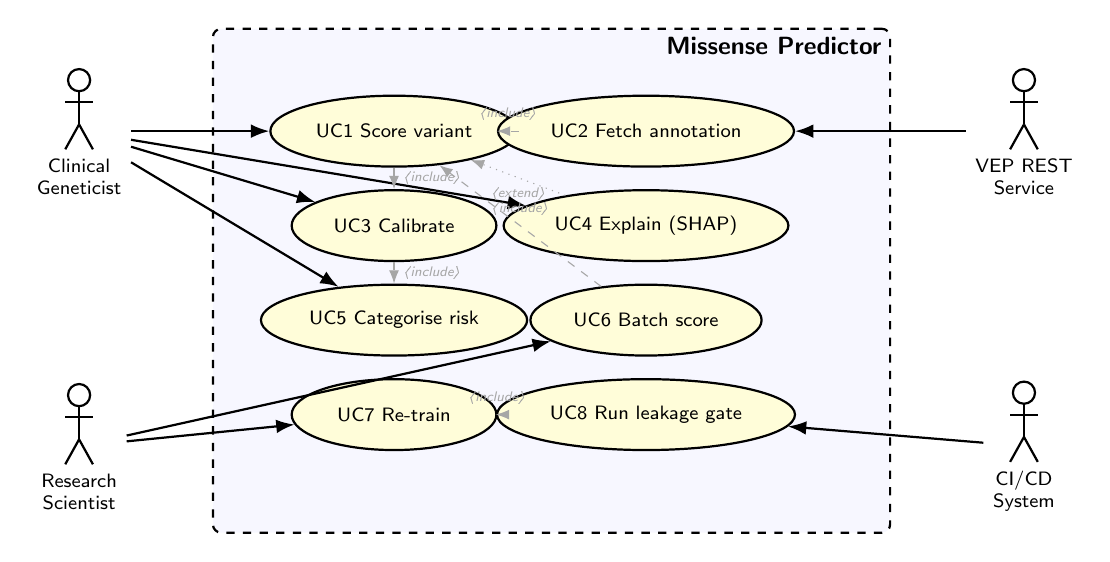
\begin{tikzpicture}[
  font=\sffamily\footnotesize,
  actor/.style={font=\sffamily\scriptsize, align=center},
  uc/.style={draw, ellipse, minimum width=2.6cm, minimum height=0.9cm,
    align=center, thick, fill=yellow!15, font=\sffamily\scriptsize},
  sys/.style={draw, rounded corners=3pt, thick, inner sep=0.3cm,
    fill=blue!3, dashed},
  rel/.style={-Latex, thick},
  inc/.style={-Latex, dashed, gray!70},
  ext/.style={-Latex, dotted, gray!70},
]
  % Stick-figure UML actors
  \node[actor] (g) at (-4, 2)  {\actorstick{} \\[2pt] Clinical\\Geneticist};
  \node[actor] (r) at (-4, -2) {\actorstick{} \\[2pt] Research\\Scientist};
  \node[actor] (v) at (8, 2)   {\actorstick{} \\[2pt] VEP REST\\Service};
  \node[actor] (c) at (8, -2)  {\actorstick{} \\[2pt] CI/CD\\System};

  % System boundary
  \begin{scope}[on background layer]
    \node[sys, fit={(-2, 3) (6, -2.8)}] (bnd) {};
    \node[font=\sffamily\small\bfseries, anchor=north east] at (bnd.north east) {Missense Predictor};
  \end{scope}

  \node[uc] (u1) at (0,    2)    {UC1 Score variant};
  \node[uc] (u2) at (3.2,  2)    {UC2 Fetch annotation};
  \node[uc] (u3) at (0,    0.8)  {UC3 Calibrate};
  \node[uc] (u4) at (3.2,  0.8)  {UC4 Explain (SHAP)};
  \node[uc] (u5) at (0,   -0.4)  {UC5 Categorise risk};
  \node[uc] (u6) at (3.2, -0.4)  {UC6 Batch score};
  \node[uc] (u7) at (0,   -1.6)  {UC7 Re-train};
  \node[uc] (u8) at (3.2, -1.6)  {UC8 Run leakage gate};

  % Associations (solid)
  \foreach \a/\b in {g/u1, g/u3, g/u4, g/u5, r/u6, r/u7, v/u2, c/u8}
    \draw[rel] (\a) -- (\b);

  % Include / extend
  \draw[inc] (u1) -- (u2) node[midway, above, font=\sffamily\tiny, gray!70]
       {\textit{\textlangle include\textrangle}};
  \draw[inc] (u1) -- (u3) node[midway, right, font=\sffamily\tiny, gray!70]
       {\textit{\textlangle include\textrangle}};
  \draw[inc] (u3) -- (u5) node[midway, right, font=\sffamily\tiny, gray!70]
       {\textit{\textlangle include\textrangle}};
  \draw[ext] (u4) -- (u1) node[midway, below, font=\sffamily\tiny, gray!70]
       {\textit{\textlangle extend\textrangle}};
  \draw[inc] (u6) -- (u1) node[midway, above, font=\sffamily\tiny, gray!70]
       {\textit{\textlangle include\textrangle}};
  \draw[inc] (u7) -- (u8) node[midway, above, font=\sffamily\tiny, gray!70]
       {\textit{\textlangle include\textrangle}};
\end{tikzpicture}}
\caption[Use case diagram]{\textbf{Use-case diagram.}
Actors on the outside of the system boundary; eight use
cases on the inside. Solid lines are associations; dashed
lines are $\langle\!\langle include\rangle\!\rangle$
relationships; dotted lines are
$\langle\!\langle extend\rangle\!\rangle$.}
\label{fig:uc}
\end{figure}

\subsection{Class Diagram}
\label{sec:uml-class}

Figure~\ref{fig:class} reveals the static structure of the
\texttt{src/} package. Classes are grouped into four
coloured \emph{packages} corresponding directly to the
\texttt{src/} sub-directories
\citep{martin2017cleanarch}. Each class is rendered as a
three-compartment rectangle: the class name on top, the
key attributes in the middle, and the principal methods at
the bottom. Associations carry multiplicities; the
\texttt{LeakageGate} class has a \emph{composition} (filled
diamond) with each of its four invariant checkers because
the gate does not exist meaningfully without them.

\begin{figure}[htbp]
\centering
\resizebox{\linewidth}{!}{%
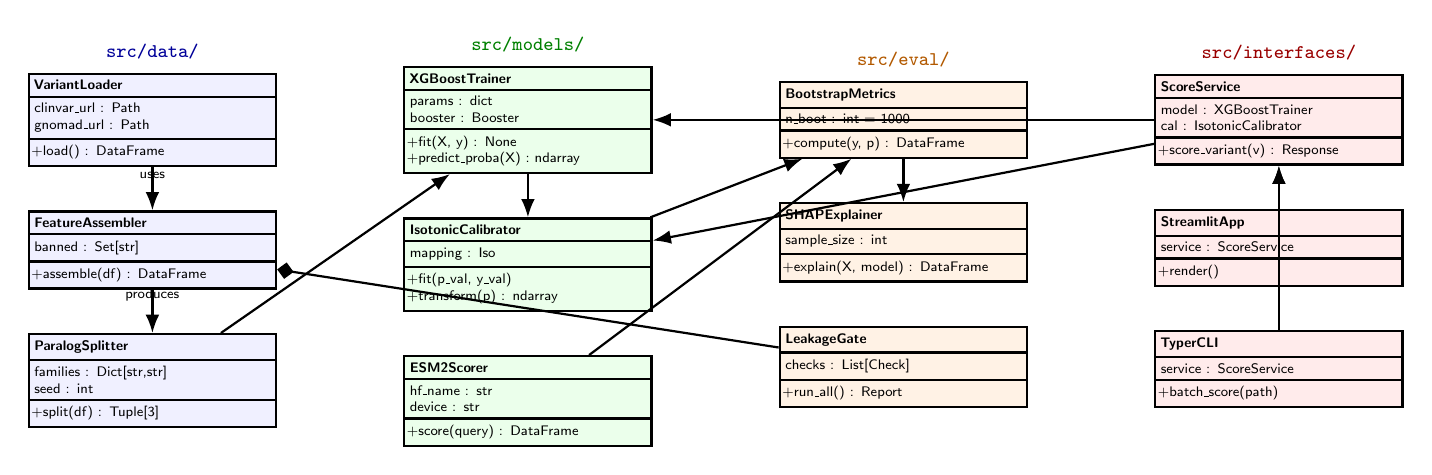
\begin{tikzpicture}[
  font=\sffamily\tiny,
  cls/.style={draw, rectangle split, rectangle split parts=3,
    rectangle split draw splits=true, rectangle split horizontal=false,
    thick, align=left, text width=3.0cm, inner sep=2pt,
    rectangle split part align=left, fill=white},
  data/.style={cls, fill=blue!6},
  model/.style={cls, fill=green!8},
  eval/.style={cls, fill=orange!10},
  iface/.style={cls, fill=red!8},
  rel/.style={-Latex, thick},
  comp/.style={-{Diamond[length=6pt, width=6pt, fill=black]}, thick},
]
  % Data pipeline package
  \node[data] (load) {\textbf{VariantLoader} \nodepart{second}
        clinvar\_url : Path \\ gnomad\_url : Path
        \nodepart{third}
        +load() : DataFrame};
  \node[data, below=0.55cm of load] (feat) {\textbf{FeatureAssembler} \nodepart{second}
        banned : Set[str]
        \nodepart{third}
        +assemble(df) : DataFrame};
  \node[data, below=0.55cm of feat] (split) {\textbf{ParalogSplitter} \nodepart{second}
        families : Dict[str,str] \\ seed : int
        \nodepart{third}
        +split(df) : Tuple[3]};

  % Model package
  \node[model, right=1.6cm of load] (xgb) {\textbf{XGBoostTrainer} \nodepart{second}
        params : dict \\ booster : Booster
        \nodepart{third}
        +fit(X, y) : None \\ +predict\_proba(X) : ndarray};
  \node[model, below=0.55cm of xgb] (cal)  {\textbf{IsotonicCalibrator} \nodepart{second}
        mapping : Iso
        \nodepart{third}
        +fit(p\_val, y\_val) \\ +transform(p) : ndarray};
  \node[model, below=0.55cm of cal] (esm)  {\textbf{ESM2Scorer} \nodepart{second}
        hf\_name : str \\ device : str
        \nodepart{third}
        +score(query) : DataFrame};

  % Eval package
  \node[eval, right=1.6cm of xgb] (boot) {\textbf{BootstrapMetrics} \nodepart{second}
        n\_boot : int = 1000
        \nodepart{third}
        +compute(y, p) : DataFrame};
  \node[eval, below=0.55cm of boot] (shap) {\textbf{SHAPExplainer} \nodepart{second}
        sample\_size : int
        \nodepart{third}
        +explain(X, model) : DataFrame};
  \node[eval, below=0.55cm of shap] (gate) {\textbf{LeakageGate} \nodepart{second}
        checks : List[Check]
        \nodepart{third}
        +run\_all() : Report};

  % Interface package
  \node[iface, right=1.6cm of boot] (app) {\textbf{ScoreService} \nodepart{second}
        model : XGBoostTrainer \\ cal : IsotonicCalibrator
        \nodepart{third}
        +score\_variant(v) : Response};
  \node[iface, below=0.55cm of app] (web) {\textbf{StreamlitApp} \nodepart{second}
        service : ScoreService
        \nodepart{third}
        +render()};
  \node[iface, below=0.55cm of web] (cli) {\textbf{TyperCLI} \nodepart{second}
        service : ScoreService
        \nodepart{third}
        +batch\_score(path)};

  % Associations
  \draw[rel] (load) -- node[above, font=\sffamily\tiny]{uses} (feat);
  \draw[rel] (feat) -- node[above, font=\sffamily\tiny]{produces} (split);
  \draw[rel] (split) -- (xgb);
  \draw[rel] (xgb) -- (cal);
  \draw[rel] (cal) -- (boot);
  \draw[rel] (boot) -- (shap);
  \draw[rel] (esm) -- (boot);
  \draw[rel] (app) -- (xgb);
  \draw[rel] (app) -- (cal);
  \draw[rel] (web) -- (app);
  \draw[rel] (cli) -- (app);
  % Composition: LeakageGate composes four checks (shown as one arrow representative)
  \draw[comp] (gate) -- (feat);

  % Package boundary labels
  \node[font=\sffamily\scriptsize\bfseries, blue!60!black, above=0.05cm of load] {\texttt{src/data/}};
  \node[font=\sffamily\scriptsize\bfseries, green!50!black, above=0.05cm of xgb] {\texttt{src/models/}};
  \node[font=\sffamily\scriptsize\bfseries, orange!70!black, above=0.05cm of boot] {\texttt{src/eval/}};
  \node[font=\sffamily\scriptsize\bfseries, red!60!black, above=0.05cm of app] {\texttt{src/interfaces/}};
\end{tikzpicture}}
\caption[Class diagram]{\textbf{Class diagram.} Four
packages align one-to-one with \texttt{src/}
sub-directories. A filled diamond denotes composition:
\texttt{LeakageGate} owns the life of its invariant checks.
Open arrows are directed associations with the
\emph{uses/produces} roles labelled inline.}
\label{fig:class}
\end{figure}

\subsection{Sequence Diagram}
\label{sec:uml-sequence}

Figure~\ref{fig:seq} traces a single \texttt{score\_variant}
request through the five participants
\texttt{StreamlitApp}, \texttt{ScoreService},
\texttt{FeatureCache}, \texttt{XGBoostTrainer}, and
\texttt{SHAPExplainer}. The cache-miss branch contains a
nested \texttt{opt} fragment that calls out to the
external VEP REST service; the self-loop inside
\texttt{ScoreService} represents isotonic calibration,
which is a pure in-memory transform.

\begin{figure}[htbp]
\centering
\resizebox{\linewidth}{!}{%
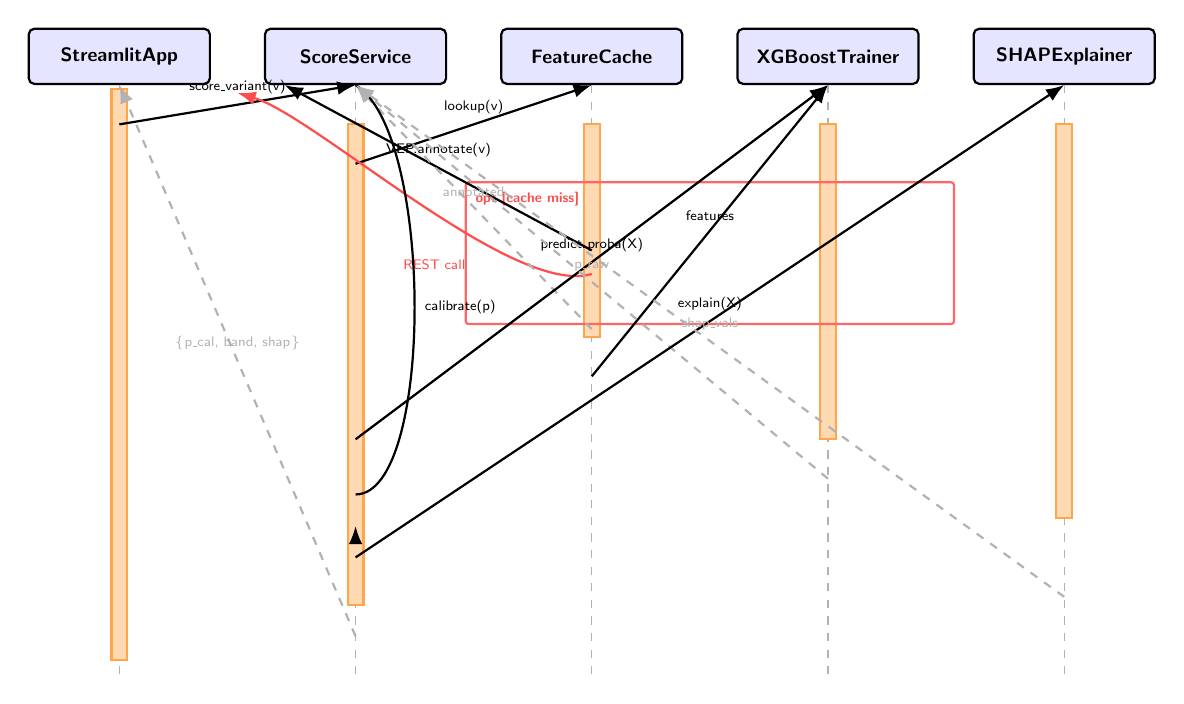
\begin{tikzpicture}[
  font=\sffamily\footnotesize,
  participant/.style={draw, rounded corners=2pt, fill=blue!10,
    minimum width=2.3cm, minimum height=0.7cm, thick, align=center,
    font=\sffamily\scriptsize\bfseries},
  lifeline/.style={dashed, gray!60},
  activation/.style={fill=orange!30, draw=orange!70, thick},
  msg/.style={-Latex, thick},
  ret/.style={-Latex, dashed, gray!60, thick},
  frag/.style={draw=red!60, thick, rounded corners=1pt},
]
  % Participants at top
  \node[participant] (a) at (0, 0)  {StreamlitApp};
  \node[participant] (s) at (3, 0)  {ScoreService};
  \node[participant] (c) at (6, 0)  {FeatureCache};
  \node[participant] (m) at (9, 0)  {XGBoostTrainer};
  \node[participant] (e) at (12, 0) {SHAPExplainer};

  % Lifelines
  \foreach \p in {a, s, c, m, e} \draw[lifeline] (\p.south) -- ++(0, -7.5);

  % Activations (coloured rectangles on lifelines)
  \fill[activation] (a.south)+(-0.1, -0.05) rectangle ++(0.1, -7.3);
  \fill[activation] (s.south)+(-0.1, -0.5) rectangle ++(0.1, -6.6);
  \fill[activation] (c.south)+(-0.1, -1.0) rectangle ++(0.1, -0.8);
  \fill[activation] (c.south)+(-0.1, -3.2) rectangle ++(0.1, -0.5);
  \fill[activation] (m.south)+(-0.1, -4.5) rectangle ++(0.1, -0.5);
  \fill[activation] (e.south)+(-0.1, -5.5) rectangle ++(0.1, -0.5);

  % Messages
  \draw[msg] (a.south)+(0,-0.5) -- ++(3, 0) node[midway, above, font=\sffamily\tiny]{score\_variant(v)};
  \draw[msg] (s.south)+(0,-1.0) -- ++(3, 0) node[midway, above, font=\sffamily\tiny]{lookup(v)};

  % opt frame (cache miss)
  \draw[frag] (4.4, -1.6) rectangle (10.6, -3.4);
  \node[anchor=north west, font=\sffamily\tiny\bfseries, red!70] at (4.4, -1.6) {opt [cache miss]};
  \draw[msg] (c.south)+(0,-2.1) -- ++(-3.9, 0) node[midway, above, font=\sffamily\tiny, text width=2.4cm, align=center]{VEP.annotate(v)};
  \draw[msg, red!70] (c.south)+(0,-2.4) .. controls ++(-1, -0.3) and ++(1, -0.3) .. ++(-4.5, -0.1);
  \node[font=\sffamily\tiny, red!70] at (4, -2.65) {REST call};
  \draw[ret] (c.south)+(0,-3.1) -- ++(-3, 0) node[midway, above, font=\sffamily\tiny]{annotated};

  \draw[msg] (c.south)+(0,-3.7) -- ++(3, 0) node[midway, above, font=\sffamily\tiny]{features};
  \draw[msg] (s.south)+(0,-4.5) -- ++(6, 0) node[midway, above, font=\sffamily\tiny]{predict\_proba(X)};
  \draw[ret] (m.south)+(0,-5.0) -- ++(-6, 0) node[midway, above, font=\sffamily\tiny]{p\_raw};

  % self-loop for calibration
  \draw[msg] (s.south)+(0,-5.2) .. controls ++(1, 0) and ++(1, -0.6) .. (s.south)+(0,-5.6)
    node[midway, right, font=\sffamily\tiny]{calibrate(p)};

  \draw[msg] (s.south)+(0,-6.0) -- ++(9, 0) node[midway, above, font=\sffamily\tiny]{explain(X)};
  \draw[ret] (e.south)+(0,-6.5) -- ++(-9, 0) node[midway, above, font=\sffamily\tiny]{shap\_vals};

  \draw[ret] (s.south)+(0,-7.0) -- ++(-3, 0) node[midway, above, font=\sffamily\tiny]{\{p\_cal, band, shap\}};
\end{tikzpicture}}
\caption[Sequence diagram]{\textbf{Sequence diagram for a
single scoring request.} Orange bars are activation
frames; red frame is an \texttt{opt} fragment for the
cache-miss branch (adds $\sim$1--2~s latency). Self-loop on
\texttt{ScoreService} denotes isotonic calibration.}
\label{fig:seq}
\end{figure}

\subsection{Activity Diagram}
\label{sec:uml-activity}

Figure~\ref{fig:act} models the \emph{training and
evaluation} workflow as an activity diagram with explicit
\emph{fork} and \emph{join} pseudo-nodes. The two fork/join
pairs capture the two independent parallelisations in the
pipeline: the leakage gate runs four checks concurrently
(fork-1 / join-1) and the evaluation step runs five
independent scoring tracks concurrently (fork-2 / join-2).

\begin{figure}[htbp]
\centering
\resizebox{\linewidth}{!}{%
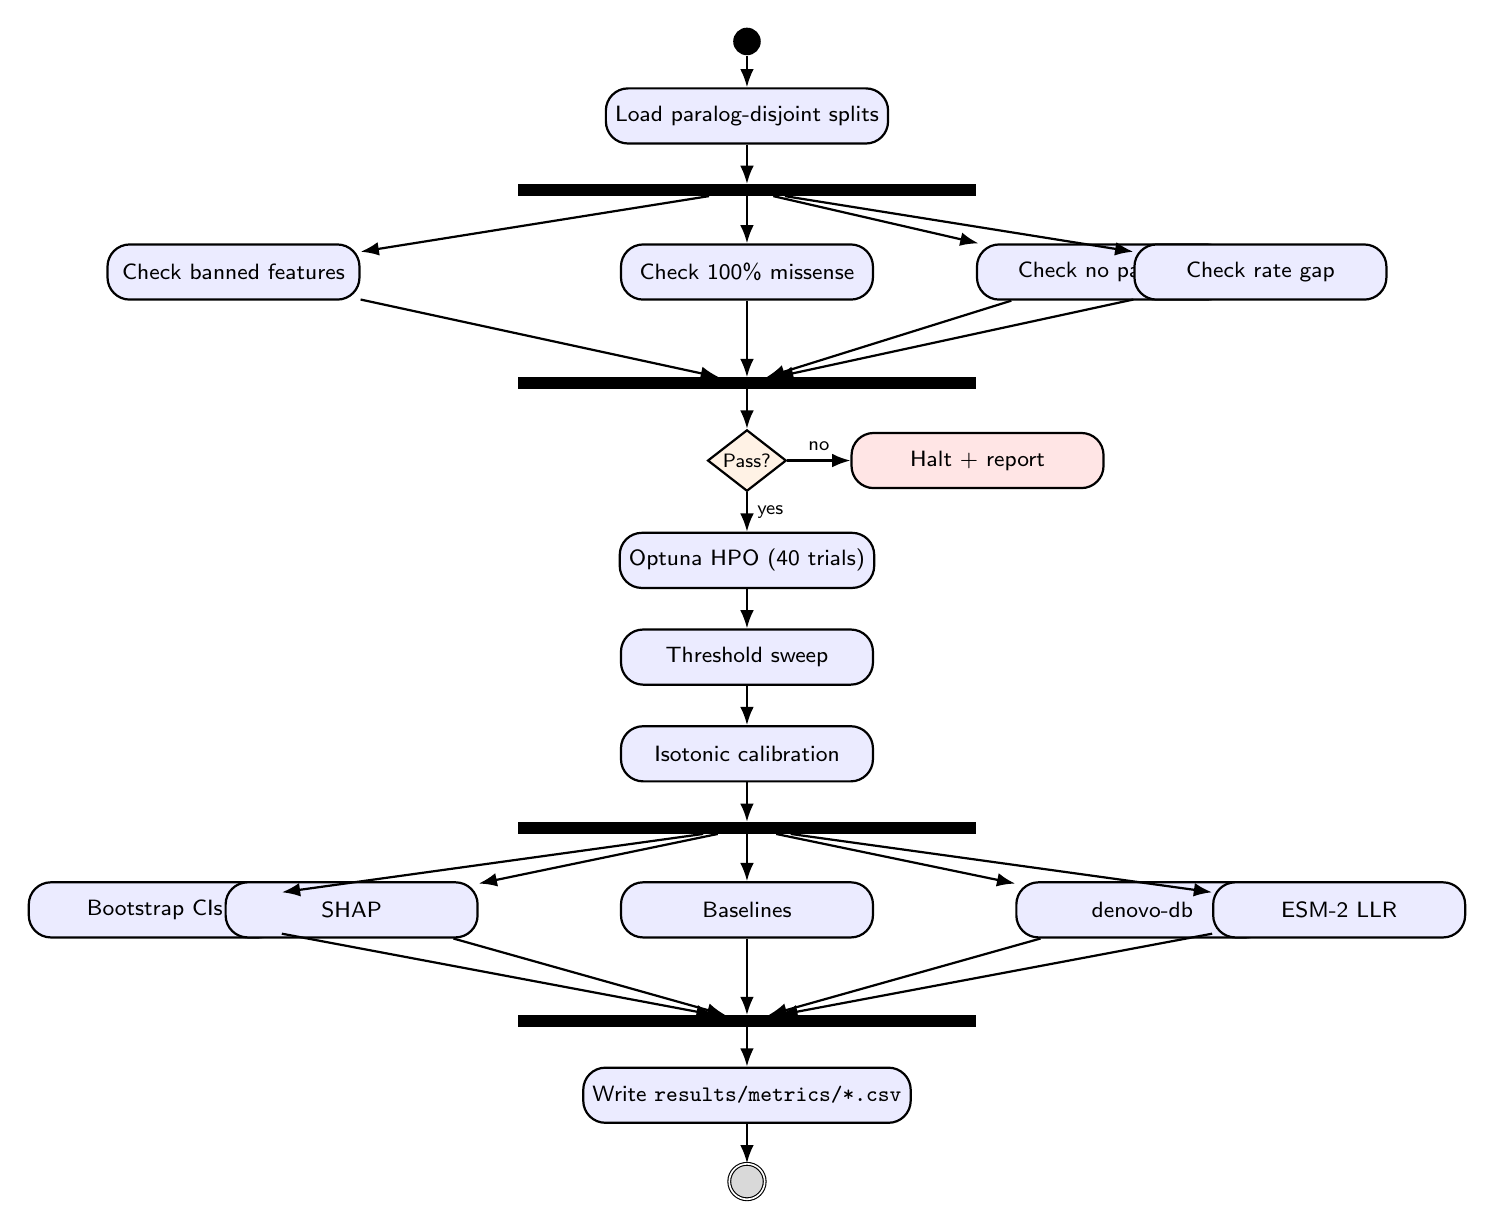
\begin{tikzpicture}[
  font=\sffamily\footnotesize,
  start/.style={circle, fill=black, minimum size=0.35cm, inner sep=0pt},
  stop/.style={circle, draw=black, double, minimum size=0.45cm, inner sep=0pt,
    fill=black!15},
  act/.style={draw, rounded corners=8pt, minimum width=3.2cm,
    minimum height=0.7cm, align=center, thick, fill=blue!8},
  dec/.style={diamond, draw, minimum width=1.0cm, minimum height=0.7cm,
    inner sep=0pt, fill=orange!10, thick, font=\sffamily\scriptsize, align=center},
  fork/.style={rectangle, draw=black, fill=black, minimum height=0.14cm,
    minimum width=5.8cm, inner sep=0pt},
  arrow/.style={-Latex, thick},
]
  \node[start] (s) at (0, 0) {};
  \node[act, below=0.4cm of s] (load) {Load paralog-disjoint splits};

  \node[fork, below=0.5cm of load] (f1) {};
  \node[act, below left=0.6cm and 2.0cm of f1] (ch1) {Check banned features};
  \node[act, below=0.6cm of f1]             (ch2) {Check 100\% missense};
  \node[act, below right=0.6cm and 0.0cm of f1] (ch3) {Check no paralog};
  \node[act, below right=0.6cm and 2.0cm of f1] (ch4) {Check rate gap};
  \node[fork, below=2.3cm of f1] (j1) {};

  \node[dec, below=0.5cm of j1] (d1) {Pass?};
  \node[act, right=0.8cm of d1, fill=red!10] (halt) {Halt + report};

  \node[act, below=0.5cm of d1] (opt) {Optuna HPO (40 trials)};
  \node[act, below=0.5cm of opt] (thr) {Threshold sweep};
  \node[act, below=0.5cm of thr] (cal) {Isotonic calibration};

  \node[fork, below=0.5cm of cal] (f2) {};
  \node[act, below left=0.6cm and 3cm of f2]  (t1) {Bootstrap CIs};
  \node[act, below left=0.6cm and 0.5cm of f2]  (t2) {SHAP};
  \node[act, below=0.6cm of f2]                 (t3) {Baselines};
  \node[act, below right=0.6cm and 0.5cm of f2] (t4) {denovo-db};
  \node[act, below right=0.6cm and 3cm of f2]   (t5) {ESM-2 LLR};
  \node[fork, below=2.3cm of f2] (j2) {};

  \node[act, below=0.5cm of j2] (rep) {Write \texttt{results/metrics/*.csv}};
  \node[stop, below=0.5cm of rep] (e) {};

  \draw[arrow] (s) -- (load);
  \draw[arrow] (load) -- (f1);
  \draw[arrow] (f1) -- (ch1);
  \draw[arrow] (f1) -- (ch2);
  \draw[arrow] (f1) -- (ch3);
  \draw[arrow] (f1) -- (ch4);
  \draw[arrow] (ch1) -- (j1);
  \draw[arrow] (ch2) -- (j1);
  \draw[arrow] (ch3) -- (j1);
  \draw[arrow] (ch4) -- (j1);
  \draw[arrow] (j1) -- (d1);
  \draw[arrow] (d1) -- (halt) node[midway, above, font=\sffamily\scriptsize]{no};
  \draw[arrow] (d1) -- (opt) node[midway, right, font=\sffamily\scriptsize]{yes};
  \draw[arrow] (opt) -- (thr);
  \draw[arrow] (thr) -- (cal);
  \draw[arrow] (cal) -- (f2);
  \draw[arrow] (f2) -- (t1);
  \draw[arrow] (f2) -- (t2);
  \draw[arrow] (f2) -- (t3);
  \draw[arrow] (f2) -- (t4);
  \draw[arrow] (f2) -- (t5);
  \foreach \x in {t1, t2, t3, t4, t5} \draw[arrow] (\x) -- (j2);
  \draw[arrow] (j2) -- (rep);
  \draw[arrow] (rep) -- (e);
\end{tikzpicture}}
\caption[Activity diagram]{\textbf{Activity diagram} for the
training + evaluation workflow. The two thick black bars
are fork/join pseudo-nodes: Fork-1 runs the four leakage
checks in parallel; Fork-2 runs the five evaluation tracks
in parallel. If any leakage check fails, execution halts
without touching the training stage.}
\label{fig:act}
\end{figure}

\subsection{State Diagram}
\label{sec:uml-state}

Figure~\ref{fig:state} captures the life-cycle of a single
variant as it moves through the pipeline. The variant
enters the \texttt{Submitted} state, transits
\texttt{Annotated} (after feature assembly) and
\texttt{Scored} (after XGBoost), is then
\texttt{Calibrated} (after isotonic), and finally
\texttt{Classified} into one of the three risk bands.
A dotted transition to the \texttt{Failed} terminal state
captures any error raised by the VEP round-trip or by the
type validator.

\begin{figure}[htbp]
\centering
\resizebox{\linewidth}{!}{%
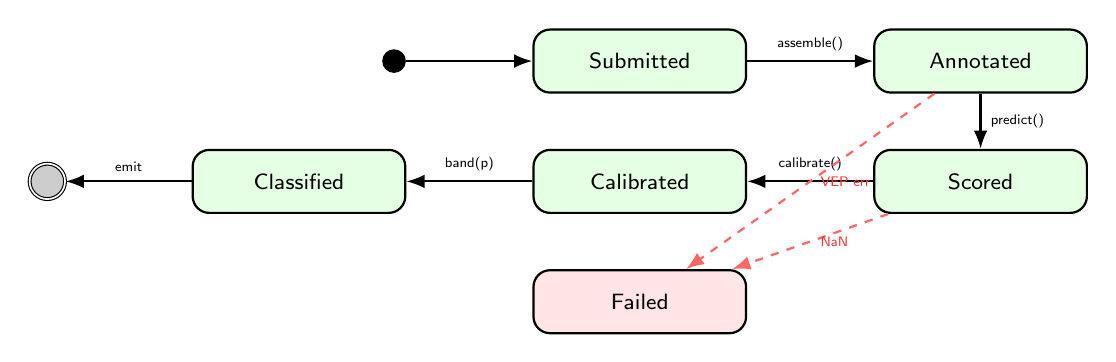
\begin{tikzpicture}[
  font=\sffamily\footnotesize,
  node distance=0.7cm and 1.6cm,
  st/.style={draw, rounded corners=6pt, minimum width=2.7cm,
    minimum height=0.8cm, align=center, thick, fill=green!10},
  term/.style={st, fill=red!10},
  init/.style={circle, fill=black, minimum size=0.3cm, inner sep=0pt},
  final/.style={circle, draw=black, double, minimum size=0.45cm,
    inner sep=0pt, fill=black!20},
  arrow/.style={-Latex, thick},
]
  \node[init] (s) {};
  \node[st, right=of s] (sub) {Submitted};
  \node[st, right=of sub] (ann) {Annotated};
  \node[st, below=of ann] (sc)  {Scored};
  \node[st, left=of sc]   (cal) {Calibrated};
  \node[st, left=of cal]  (cls) {Classified};
  \node[term, below=of cal] (fail) {Failed};
  \node[final, left=of cls] (e) {};

  \draw[arrow] (s) -- (sub);
  \draw[arrow] (sub) -- node[above, font=\sffamily\tiny]{assemble()} (ann);
  \draw[arrow] (ann) -- node[right, font=\sffamily\tiny]{predict()} (sc);
  \draw[arrow] (sc)  -- node[above, font=\sffamily\tiny]{calibrate()} (cal);
  \draw[arrow] (cal) -- node[above, font=\sffamily\tiny]{band(p)} (cls);
  \draw[arrow] (cls) -- node[above, font=\sffamily\tiny]{emit} (e);
  \draw[arrow, dashed, red!60] (ann) -- node[right, font=\sffamily\tiny, red!80]{VEP err} (fail);
  \draw[arrow, dashed, red!60] (sc)  -- node[right, font=\sffamily\tiny, red!80]{NaN} (fail);
\end{tikzpicture}}
\caption[State diagram]{\textbf{State diagram for a
variant's life-cycle.} Every successful variant follows
the five-state green path. Dashed red transitions lead to
\texttt{Failed}; the terminal double-circle indicates the
final reported state.}
\label{fig:state}
\end{figure}

\subsection{Component Diagram}
\label{sec:uml-component}

Figure~\ref{fig:comp} shows the component-level view with
provided/required interfaces (UML ``ball and socket''
notation). Internal components are drawn as rectangles
with the UML component icon; external services (VEP,
HuggingFace Hub, gnomAD FTP) are drawn as cloud shapes.
Every arrow in the diagram corresponds either to a
concrete Python import or to an HTTP/FTP call.

\begin{figure}[htbp]
\centering
\resizebox{\linewidth}{!}{%
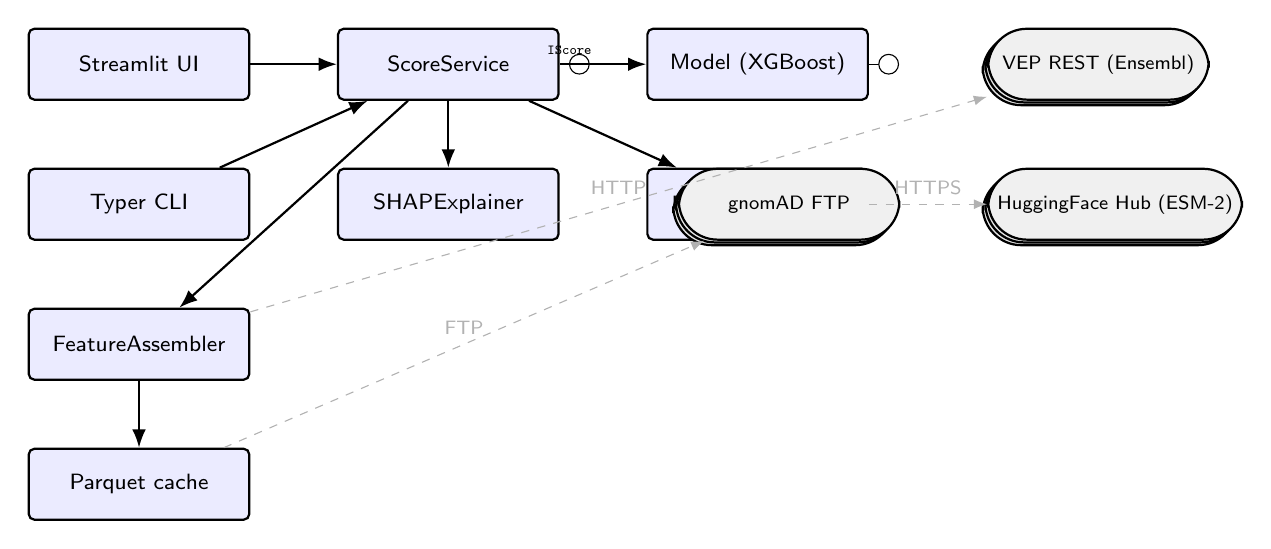
\begin{tikzpicture}[
  font=\sffamily\footnotesize,
  node distance=0.85cm and 1.1cm,
  comp/.style={draw, thick, rounded corners=2pt, minimum width=2.8cm,
    minimum height=0.9cm, align=center, fill=blue!8},
  ext/.style={draw, thick, rounded corners=14pt, minimum width=2.8cm,
    minimum height=0.9cm, fill=gray!12, align=center,
    font=\sffamily\scriptsize, double copy shadow={shadow xshift=-1pt, shadow yshift=-1pt, fill=gray!20}},
  prov/.style={circle, draw=black, fill=white, minimum size=0.25cm, inner sep=0pt},
  arrow/.style={-Latex, thick},
  dep/.style={-Latex, dashed, gray!60},
]
  % Internal components (left)
  \node[comp] (sl)  {Streamlit UI};
  \node[comp, below=of sl] (cli) {Typer CLI};
  \node[comp, right=of sl] (svc) {ScoreService};
  \node[comp, right=of svc] (mdl) {Model (XGBoost)};
  \node[comp, below=of mdl] (cal) {IsotonicCalibrator};
  \node[comp, below=of svc] (shap) {SHAPExplainer};
  \node[comp, below=of cli] (data) {FeatureAssembler};
  \node[comp, below=of data] (cache) {Parquet cache};

  % External services (right side, rounded boxes emulating clouds)
  \node[ext, right=1.5cm of mdl] (vep)  {VEP REST (Ensembl)};
  \node[ext, right=1.5cm of cal] (hf)   {HuggingFace Hub (ESM-2)};
  \node[ext, right=1.5cm of shap] (gnom) {gnomAD FTP};

  % Provided / required at interfaces (decorative)
  \draw (svc.east) -- node[above, font=\sffamily\tiny]{\texttt{IScore}} ++(0.25, 0)
    node[prov]{};
  \draw (mdl.east) -- ++(0.25, 0) node[prov]{};

  % Module imports (thin solid arrows)
  \draw[arrow] (sl)  -- (svc);
  \draw[arrow] (cli) -- (svc);
  \draw[arrow] (svc) -- (mdl);
  \draw[arrow] (svc) -- (cal);
  \draw[arrow] (svc) -- (shap);
  \draw[arrow] (svc) -- (data);
  \draw[arrow] (data) -- (cache);

  % External HTTP / FTP dependencies
  \draw[dep] (data) -- node[above, font=\sffamily\scriptsize]{HTTP} (vep);
  \draw[dep] (cal) -- node[above, font=\sffamily\scriptsize]{HTTPS} (hf);
  \draw[dep] (cache) -- node[above, font=\sffamily\scriptsize]{FTP} (gnom);
\end{tikzpicture}}
\caption[Component diagram]{\textbf{Component diagram.}
Components with the UML component icon (rounded rectangle)
are internal Python modules; cloud icons are external
network services. Solid arrows are Python imports; dashed
arrows are network dependencies.}
\label{fig:comp}
\end{figure}

\section{Interface Design}
\label{sec:an-iface}

\subsection{Streamlit Web Interface}
The Streamlit application (Figure~\ref{fig:streamlit})
provides a single-page interactive experience. A user
enters a variant in \texttt{chr:pos:ref:alt} form,
presses \emph{Score variant}, and receives the
calibrated probability, a coloured risk banner, and the
top-$15$ SHAP contributions as a signed bar chart.

\begin{figure}[H]
\centering
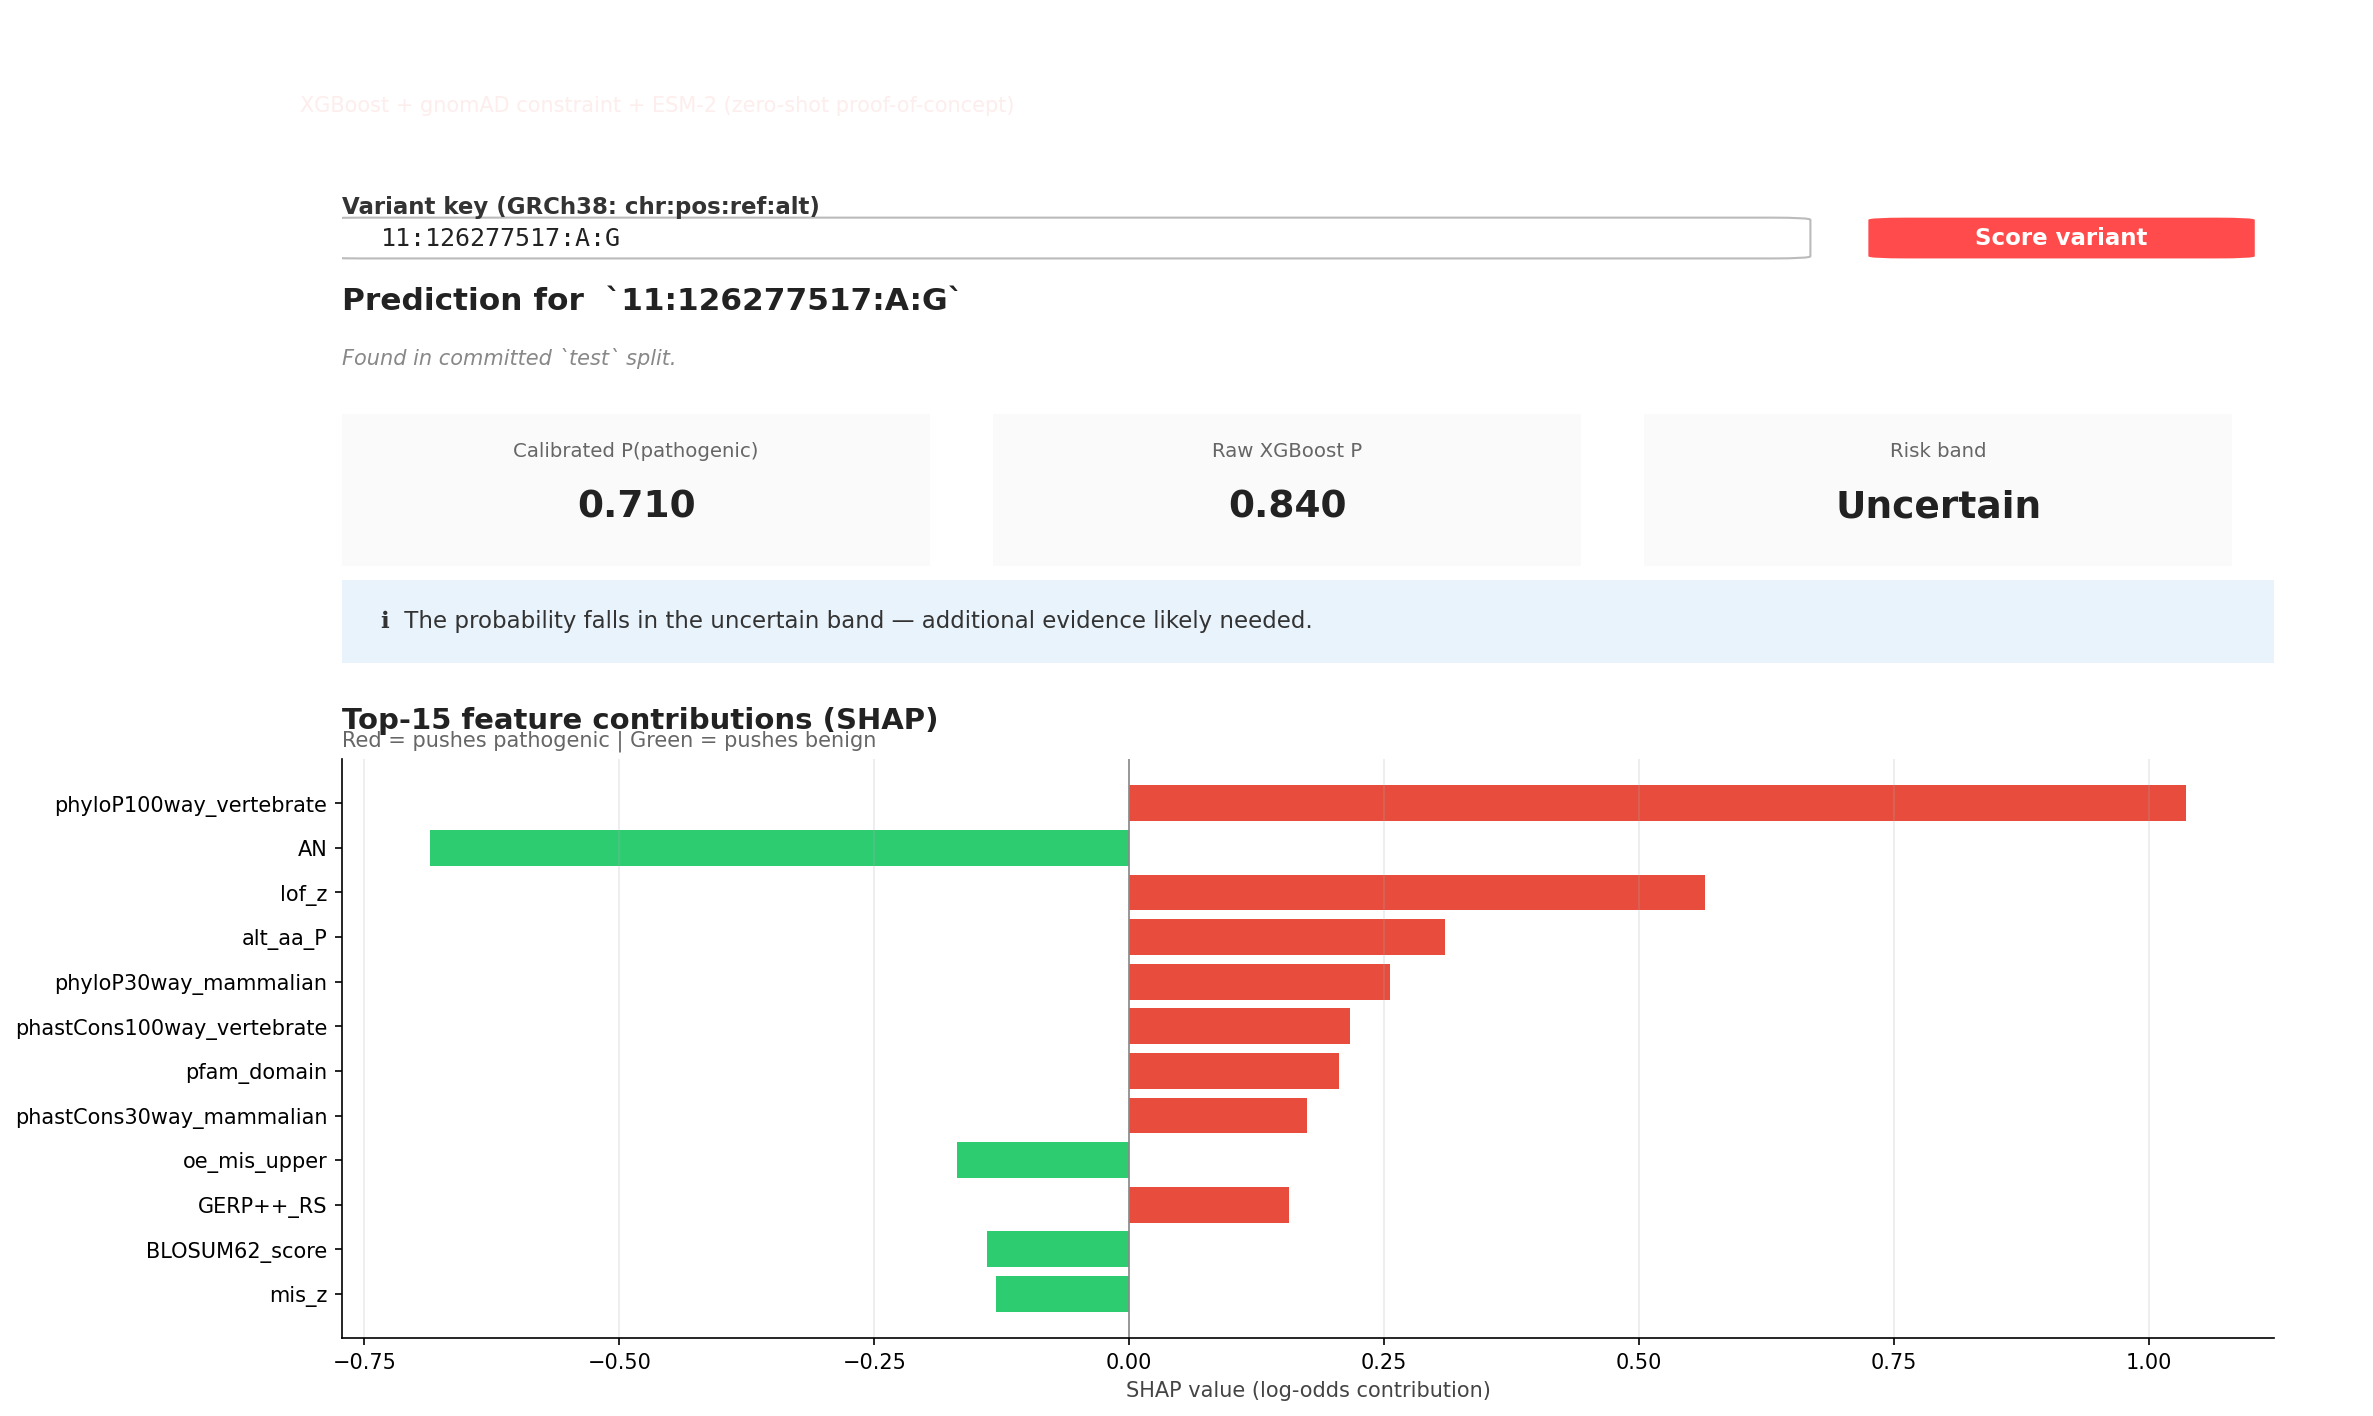
\includegraphics[width=0.95\linewidth]{figures/screenshots/07_streamlit_demo.png}
\caption[Streamlit demo interface]{Streamlit demo
interface rendering a real prediction for a test-set
variant. Red SHAP bars push the prediction towards
pathogenic, green bars towards benign.}
\label{fig:streamlit}
\end{figure}

\subsection{Command-Line Interface}
The CLI layer lives in \texttt{scripts/} and exposes
every pipeline step as an independent command:
\texttt{run\_baselines.py},
\texttt{evaluate\_external.py},
\texttt{compute\_shap.py}, and so on. Common arguments
(\texttt{--n-boot}, \texttt{--seed}, \texttt{--only})
are harmonised across scripts.

\subsection{Programmatic API}
The \texttt{src/} package itself constitutes a stable
Python API. Key entry points include
\texttt{score\_variants()} in
\texttt{src/\allowbreak esm2\_scorer.py} and
\texttt{evaluate\_baseline()} in
\texttt{src/\allowbreak baselines/\allowbreak evaluate.py}.

\section{Summary}
\label{sec:an-summary}

The functional and non-functional requirements,
together with the six UML diagrams, formalise the
software architecture introduced in
Chapter~\ref{ch:framework}. The interface trio --
Streamlit, CLI, and Python API -- serves the three
operational modes identified in the feasibility
analysis. Chapter~\ref{ch:implementation} reports
how these designs translate into concrete code and
what results they produce.

% ═════════════════════════════════════════════════════════════════════════
%   CHAPTER 5 — IMPLEMENTATION AND RESULTS
% ═════════════════════════════════════════════════════════════════════════

\chapter{Implementation and Results}
\label{ch:implementation}

\section{Introduction}
\label{sec:impl-intro}

This chapter is the empirical core of the thesis. It begins
with the hardware and software environment
(Sections~\ref{sec:impl-hw}--\ref{sec:impl-sw}), then
formalises the two model architectures the project actually
trained -- the gradient-boosted tree baseline and the
protein-language-model scorer -- together with the rank-
fusion operator that combines them
(Section~\ref{sec:impl-models}). The seven most important
code fragments that realise those designs are walked through
in Section~\ref{sec:impl-details}. The quantitative results
then follow in a fixed narrative order
(Section~\ref{sec:impl-results}): headline test-set metrics,
the five-stage leakage-fix journey, a like-for-like
comparison against SIFT, PolyPhen-2, and AlphaMissense, a
calibration deep-dive with the Murphy decomposition, SHAP
interpretability and confident-error analysis, external
validation on \textsc{denovo-db}, and the ESM-2 zero-shot
proof-of-concept with rank-fusion gain. The chapter closes
with a direct comparison against the prior work surveyed in
Chapter~\ref{ch:related} and the system screenshots that
evidence every claim.

\section{Model Architectures}
\label{sec:impl-models}

This section formalises the three computational models used
in the project and is provided separately from the code
walkthrough (Section~\ref{sec:impl-details}) so that the
mathematics and the diagrams can be read independently of
Python details. Two models are trained (XGBoost,
Section~\ref{sec:arch-xgb}; ESM-2 zero-shot,
Section~\ref{sec:arch-esm2}) and one operator is applied
on top of both (rank fusion, Section~\ref{sec:arch-fusion}).

\subsection{XGBoost Gradient-Boosted Trees}
\label{sec:arch-xgb}

XGBoost \citep{chen2016xgboost} builds an additive ensemble
of decision trees by stage-wise minimisation of a
regularised log-loss objective. Given a training set
$\{(\mathbf{x}_i, y_i)\}_{i=1}^{n}$ with
$\mathbf{x}_i \in \mathbb{R}^{39}$ and $y_i \in \{0, 1\}$
(benign / pathogenic), the model after $K$ rounds is
\begin{equation}
  \hat{y}_i^{(K)} \;=\; \sigma\!\left(\sum_{k=1}^{K} f_k(\mathbf{x}_i)\right), \qquad
  f_k \in \mathcal{F},
  \label{eq:xgb-additive}
\end{equation}
where $\sigma(z) = 1/(1 + e^{-z})$ is the logistic link and
$\mathcal{F}$ is the space of regression trees. Each round
$k$ adds the tree that most reduces the second-order Taylor
expansion of the regularised objective:
\begin{equation}
  \mathcal{L}^{(k)} \;=\;
  \sum_{i=1}^{n} \ell(y_i, \hat{y}_i^{(k-1)} + f_k(\mathbf{x}_i))
  \;+\;
  \gamma T_k + \tfrac{1}{2}\lambda\|\mathbf{w}_k\|_2^2,
  \label{eq:xgb-objective}
\end{equation}
with $T_k$ the number of leaves, $\mathbf{w}_k$ the leaf
weights, $\gamma$ the complexity penalty, and $\lambda$ the
L2 shrinkage. The hyperparameters
$\{\text{max\_depth}, \text{learning\_rate}, \gamma, \lambda, n\_\text{estimators}\}$
are tuned by Optuna (Section~\ref{sec:impl-tpe}).
Figure~\ref{fig:xgb-arch} schematises a single round of
boosting and the tree-ensemble aggregation.

\begin{figure}[htbp]
\centering
\resizebox{\linewidth}{!}{%
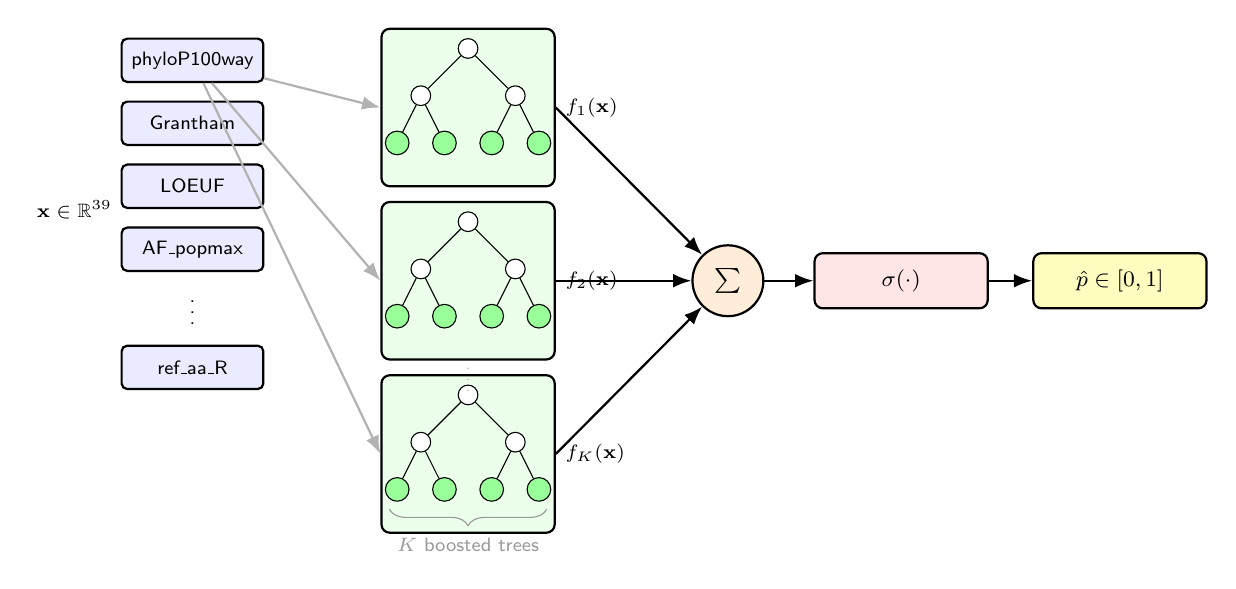
\begin{tikzpicture}[
  font=\sffamily\footnotesize,
  feat/.style={draw, rounded corners=2pt, minimum width=1.8cm,
    minimum height=0.55cm, fill=blue!8, thick, align=center,
    font=\sffamily\scriptsize},
  tree/.style={draw, rounded corners=3pt, minimum width=2.2cm,
    minimum height=2.0cm, fill=green!8, thick, align=center},
  tnode/.style={circle, draw=black, fill=white, minimum size=0.25cm,
    inner sep=0pt, font=\sffamily\tiny},
  leaf/.style={tnode, fill=green!40, minimum size=0.3cm},
  sum/.style={draw, circle, thick, fill=orange!15, minimum size=0.9cm,
    font=\sffamily\small\bfseries},
  oput/.style={draw, rounded corners=3pt, minimum width=2.2cm,
    minimum height=0.7cm, fill=red!10, thick, align=center},
  arrow/.style={-Latex, thick},
]
  % Input features (left side, stacked)
  \node[feat] (f1) at (-0.5, 3)   {phyloP100way};
  \node[feat] (f2) at (-0.5, 2.2) {Grantham};
  \node[feat] (f3) at (-0.5, 1.4) {LOEUF};
  \node[feat] (f4) at (-0.5, 0.6) {AF\_popmax};
  \node[feat, draw=none, fill=white] (fdots) at (-0.5, -0.1) {$\vdots$};
  \node[feat] (f39) at (-0.5, -0.9) {ref\_aa\_R};
  \node[font=\sffamily\scriptsize\bfseries, anchor=east] at (-1.4, 1.1) {$\mathbf{x} \in \mathbb{R}^{39}$};

  % Trees (middle)
  \foreach \i/\y in {1/2.4, 2/0.2, 3/-2} {
    \node[tree] (t\i) at (3, \y) {};
    \node[tnode] (r\i) at (3, \y+0.75) {};
    \node[tnode] (l\i) at (2.4, \y+0.15) {};
    \node[tnode] (rr\i) at (3.6, \y+0.15) {};
    \node[leaf] (ll\i) at (2.1, \y-0.45) {};
    \node[leaf] (lr\i) at (2.7, \y-0.45) {};
    \node[leaf] (rl\i) at (3.3, \y-0.45) {};
    \node[leaf] (rr2\i) at (3.9, \y-0.45) {};
    \draw (r\i) -- (l\i); \draw (r\i) -- (rr\i);
    \draw (l\i) -- (ll\i); \draw (l\i) -- (lr\i);
    \draw (rr\i) -- (rl\i); \draw (rr\i) -- (rr2\i);
  }
  \node[anchor=west, font=\sffamily\scriptsize] at (t1.east) {$f_1(\mathbf{x})$};
  \node[anchor=west, font=\sffamily\scriptsize] at (t2.east) {$f_2(\mathbf{x})$};
  \node[anchor=west, font=\sffamily\scriptsize] at (t3.east) {$f_K(\mathbf{x})$};

  \node[font=\sffamily\tiny, gray!70] at (3, -0.95) {$\vdots$};

  % Sum + sigmoid + output
  \node[sum] (s) at (6.3, 0.2) {$\sum$};
  \node[oput] (sig) at (8.5, 0.2) {$\sigma(\cdot)$};
  \node[oput, right=0.55cm of sig, fill=yellow!25] (phat) {$\hat{p}\in[0,1]$};

  % Arrows
  \foreach \i in {1, 2, 3} {
    \draw[arrow, gray!60] (f1) -- (t\i.west);
    \draw[arrow] (t\i.east) -- (s);
  }
  \draw[arrow, thick] (s) -- (sig);
  \draw[arrow, thick] (sig) -- (phat);

  % Bracket + caption
  \draw[decorate, decoration={brace, amplitude=6pt, mirror}, gray!80]
    (2.0, -2.7) -- (4.0, -2.7)
    node[midway, below=7pt, font=\sffamily\scriptsize]{$K$ boosted trees};
\end{tikzpicture}}
\caption[XGBoost architecture]{\textbf{XGBoost
architecture.} The 39-dimensional feature vector
$\mathbf{x}$ is fed independently into $K$ regression
trees; leaf outputs are summed and squashed by the
logistic $\sigma(\cdot)$ to produce a probability
$\hat p \in [0, 1]$. Optuna tuning selects $K$ together with
four structural hyperparameters.}
\label{fig:xgb-arch}
\end{figure}

\subsection{ESM-2 Zero-Shot Log-Likelihood Ratio}
\label{sec:arch-esm2}

ESM-2 \citep{lin2023esm2} is a masked-language-model
transformer \citep{vaswani2017attention} pretrained on
65~million unique UniRef sequences. The variant we use,
\texttt{esm2\_t12\_35M\_UR50D}, has
$12$ transformer blocks, an embedding dimension of $480$, a
hidden dimension of $1{,}920$, $20$ attention heads, and
approximately $35$~million parameters. We apply the model
\emph{zero-shot}: no weights are updated; only the
pretrained language-modelling head is used. For a missense
variant with reference amino acid $a_{\text{ref}}$ and
alternate $a_{\text{alt}}$ at protein position $\pi$, we
construct a windowed sequence $\tilde{s}$ (length
$\leq 1024$), replace position $\pi$ by the \texttt{MASK}
token, run one forward pass, and take the log-likelihood
ratio:
\begin{equation}
  \mathrm{LLR}_{\text{ESM-2}}(a_{\text{ref}} \to a_{\text{alt}} \mid \tilde{s})
  \;=\;
  \log \frac{\mathbb{P}_{\theta}\!\big(x_\pi = a_{\text{alt}} \mid \tilde{s}_{\backslash \pi}\big)}
           {\mathbb{P}_{\theta}\!\big(x_\pi = a_{\text{ref}} \mid \tilde{s}_{\backslash \pi}\big)}.
  \label{eq:esm2-llr}
\end{equation}
Lower (more negative) LLR implies the alternate amino acid
is less plausible under the learned language model --
i.e.\ more likely to disrupt the protein. This zero-shot
score is the exact measurement used in VariPred
\citep{lin2024varipred} and ESM-1b variant scoring
\citep{brandes2023esm1b}. Figure~\ref{fig:esm2-arch}
renders the inference path.

\begin{figure}[htbp]
\centering
\resizebox{\linewidth}{!}{%
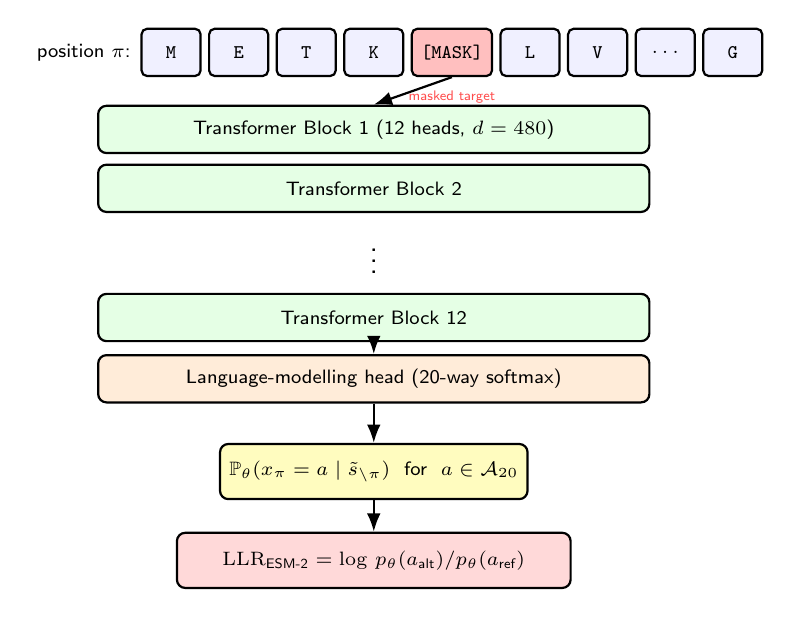
\begin{tikzpicture}[
  font=\sffamily\footnotesize,
  tok/.style={draw, rounded corners=2pt, minimum width=0.75cm,
    minimum height=0.6cm, align=center, fill=blue!6,
    font=\sffamily\scriptsize\ttfamily, thick},
  mask/.style={tok, fill=red!25, font=\sffamily\scriptsize\ttfamily\bfseries},
  block/.style={draw, rounded corners=3pt, minimum width=7.0cm,
    minimum height=0.6cm, align=center, fill=green!10, thick,
    font=\sffamily\scriptsize},
  head/.style={block, fill=orange!15},
  oput/.style={draw, rounded corners=3pt, minimum width=2.5cm,
    minimum height=0.7cm, align=center, fill=yellow!25, thick,
    font=\sffamily\scriptsize},
  arrow/.style={-Latex, thick},
]
  % Input sequence with masked position
  \node[tok] (t1) at (0, 4.2) {M};
  \node[tok, right=0.08cm of t1] (t2) {E};
  \node[tok, right=0.08cm of t2] (t3) {T};
  \node[tok, right=0.08cm of t3] (t4) {K};
  \node[mask, right=0.08cm of t4] (m)  {[MASK]};
  \node[tok, right=0.08cm of m]  (t5) {L};
  \node[tok, right=0.08cm of t5] (t6) {V};
  \node[tok, right=0.08cm of t6] (t7) {$\ldots$};
  \node[tok, right=0.08cm of t7] (t8) {G};

  \node[anchor=east, font=\sffamily\scriptsize] at (t1.west) {position $\pi$:};
  \node[below=0.05cm of m, font=\sffamily\tiny, red!70] {masked target};

  % 12 transformer blocks (stacked vertical)
  \node[block, below=0.35cm of t4] (b1) {Transformer Block 1 (12 heads, $d=480$)};
  \node[block, below=0.12cm of b1] (b2) {Transformer Block 2};
  \node[font=\sffamily\scriptsize\bfseries, below=0.12cm of b2] (dots) {$\vdots$};
  \node[block, below=0.12cm of dots] (b12) {Transformer Block 12};
  \node[head, below=0.15cm of b12] (lm) {Language-modelling head (20-way softmax)};

  % Probability output at masked position
  \node[oput, below=0.5cm of lm] (prob) {$\mathbb{P}_\theta(x_\pi = a \mid \tilde{s}_{\backslash \pi})$ \ for \ $a \in \mathcal{A}_{20}$};

  \node[oput, below=0.4cm of prob, fill=red!15, minimum width=5cm]
     (llr) {$\mathrm{LLR}_{\text{ESM-2}} = \log\, p_\theta(a_\text{alt}) / p_\theta(a_\text{ref})$};

  \draw[arrow] (m.south) -- (b1.north);
  \draw[arrow] (b12) -- (lm);
  \draw[arrow] (lm) -- (prob);
  \draw[arrow] (prob) -- (llr);
\end{tikzpicture}}
\caption[ESM-2 zero-shot scoring]{\textbf{ESM-2 zero-shot
scoring.} A windowed protein sequence with the variant
position masked is pushed through the 12 transformer
blocks and the language-modelling head. The final log-
likelihood ratio between the alternate and reference
amino acids is the single scalar score used downstream.}
\label{fig:esm2-arch}
\end{figure}

\subsection{Rank Fusion}
\label{sec:arch-fusion}

A natural question is whether the calibrated XGBoost
probability $\hat p_{\text{XGB}}$ and the ESM-2 LLR
$s_{\text{ESM}}$ carry orthogonal information or the same
signal in a different parameterisation. To test this
cheaply -- before committing to the expensive full-training-
set ESM-2 scoring -- we apply \emph{rank fusion} on the
held-out denovo-db set. Let $r_i^{\text{XGB}}$ and
$r_i^{\text{ESM}}$ be the ranks of sample $i$ under each
score (larger = more pathogenic). The fused score is
\begin{equation}
  s_i^{\text{fused}} \;=\; \alpha \cdot \frac{r_i^{\text{XGB}}}{n}
                          \;+\; (1 - \alpha) \cdot \frac{r_i^{\text{ESM}}}{n},
  \quad \alpha \in [0, 1],
  \label{eq:rank-fusion}
\end{equation}
where $n$ is the number of scored variants. $\alpha$ is
tuned on an internal split to maximise PR-AUC. Rank fusion
is deliberately the cheapest possible fusion operator -- it
requires no recalibration and no retraining -- so any
empirical gain constitutes lower-bound evidence that the two
models contain independent signal.
Figure~\ref{fig:rank-fusion} illustrates the pipeline.

\begin{figure}[htbp]
\centering
\resizebox{\linewidth}{!}{%
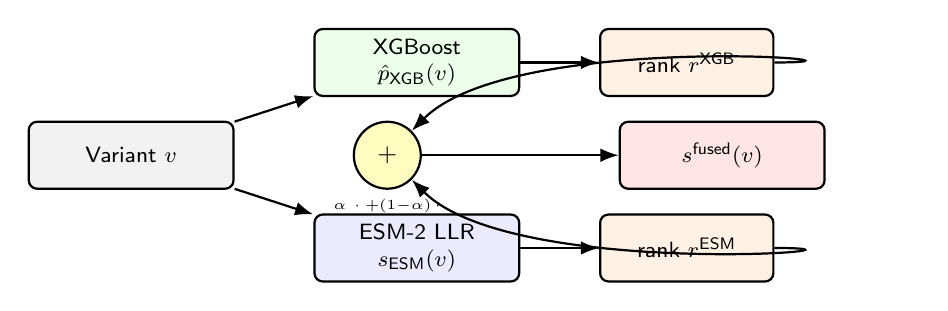
\begin{tikzpicture}[
  font=\sffamily\footnotesize,
  box/.style={draw, rounded corners=3pt, minimum width=2.6cm,
    minimum height=0.85cm, align=center, thick},
  xgb/.style={box, fill=green!8},
  esm/.style={box, fill=blue!8},
  rank/.style={box, fill=orange!10, minimum width=2.2cm},
  sum/.style={draw, circle, fill=yellow!25, thick, minimum size=0.85cm,
    font=\sffamily\small\bfseries},
  oput/.style={box, fill=red!10},
  arrow/.style={-Latex, thick},
]
  \node[box, fill=gray!10] (v) {Variant $v$};

  \node[xgb, above right=0.3cm and 1.0cm of v] (xg) {XGBoost\\$\hat p_{\text{XGB}}(v)$};
  \node[esm, below right=0.3cm and 1.0cm of v] (em) {ESM-2 LLR\\$s_{\text{ESM}}(v)$};

  \node[rank, right=of xg] (r1) {rank $r^{\text{XGB}}$};
  \node[rank, right=of em] (r2) {rank $r^{\text{ESM}}$};

  \node[sum, right=1.5cm of v] (f) {$+$};
  \node[anchor=north, font=\sffamily\tiny] at (f.south) {$\alpha\,\cdot + (1{-}\alpha)\,\cdot$};

  \node[oput, right=2.5cm of f] (fuse) {$s^{\text{fused}}(v)$};

  \draw[arrow] (v) -- (xg); \draw[arrow] (v) -- (em);
  \draw[arrow] (xg) -- (r1); \draw[arrow] (em) -- (r2);
  \draw[arrow] (r1) to[out=0, in=45] (f);
  \draw[arrow] (r2) to[out=0, in=-45] (f);
  \draw[arrow] (f) -- (fuse);
\end{tikzpicture}}
\caption[Rank-fusion pipeline]{\textbf{Rank-fusion
pipeline.} Each variant is scored independently by
XGBoost and by ESM-2; the scores are converted to ranks,
then convex-combined with a single scalar $\alpha$
tuned on an internal split.}
\label{fig:rank-fusion}
\end{figure}

\section{Hardware Environment}
\label{sec:impl-hw}

\begin{itemize}
\item \textbf{Primary development machine.} Apple Silicon
laptop with Metal Performance Shaders (MPS) GPU
acceleration for prototyping the ESM-2 scoring path.
\item \textbf{Colab compute.} A single free-tier Colab
T4 GPU session for the Phase-2.1 ESM-2 full-training-
set scoring.
\item \textbf{CI runner.} GitHub Actions
\texttt{ubuntu-22.04} for continuous integration;
deterministic identical results to the local
environment were verified through the
\texttt{test\_\allowbreak reproduce\_\allowbreak headline} integration test.
\end{itemize}

\section{Software Stack}
\label{sec:impl-sw}

\begin{itemize}
\item Python 3.11 with pinned dependencies in
\texttt{requirements-lock.txt} ($287$ packages).
\item XGBoost 2.x \citep{chen2016xgboost}, scikit-learn
1.3+, Optuna 4.x \citep{akiba2019optuna},
SHAP \citep{lundberg2017shap},
\texttt{transformers} 4.40+ and PyTorch 2.x for
ESM-2.
\item \texttt{pytest} 7.4+ with 158 unit + integration
tests \citep{pytest2024}; \texttt{ruff}, \texttt{black},
and \texttt{mypy} for code style and static typing.
\item Docker image (\texttt{Dockerfile}) based on
\texttt{python:3.11.7-slim} with \texttt{liblzma-dev}
and DSSP installed for reproducible builds.
\item GitHub Actions workflows (\texttt{test.yml},
\texttt{lint.yml}) enforcing all tests and linters on
every push to \texttt{main}.
\end{itemize}

\section{Implementation Details}
\label{sec:impl-details}

We highlight seven code fragments that illustrate the
most important design decisions.

\subsection{Paralog-Family Grouping}
\label{sec:impl-paralog}
The family grouper collapses paralog clusters under a
small set of regex rules, falling back to trailing-
digit stripping for the long tail:

\begin{lstlisting}[caption={Paralog-family assignment in \texttt{src/data\_splitting.py}.},label={lst:family}]
def assign_gene_family(gene: str) -> str:
    if gene is None:
        return ""
    g = str(gene).upper()
    for pattern, fam in _FAMILY_PATTERNS:
        m = pattern.match(g)
        if m:
            return fam if fam is not None else m.group(1)
    stripped = _TRAILING_DIGITS.sub("", g)
    return stripped or g
\end{lstlisting}

\subsection{gnomAD Constraint Merge with Train-Only Imputation}
\label{sec:impl-constraint}
The constraint merge fits imputation medians only on
the training split -- the invariant that makes this a
legal feature addition rather than a leakage:

\begin{lstlisting}[caption={Train-only median imputation in \texttt{src/gnomad\_constraint.py}.},label={lst:constraint}]
def merge_constraint(variants, *, constraint, impute_medians=None):
    merged = variants.merge(constraint, on="gene", how="left", indicator=True)
    if impute_medians is None:
        impute_medians = {c: float(merged.loc[merged["_merge"] == "both", c].median())
                          for c in CONSTRAINT_COLS if c in merged.columns}
    for c in CONSTRAINT_COLS:
        if c in merged.columns:
            merged[c] = merged[c].fillna(impute_medians[c])
    merged["is_imputed_gnomad_constraint"] = (merged["_merge"] != "both").astype(int)
    merged = merged.drop(columns="_merge")
    return merged, impute_medians
\end{lstlisting}

\subsection{Leakage Gate}
\label{sec:impl-leakage}
Four independent checks constitute the gate, wrapped in
both a CLI and a pytest test file:

\begin{lstlisting}[caption={Banned-feature check in \texttt{src/verify\_no\_leakage.py}.},label={lst:leakage}]
BANNED_FEATURES = {"is_common", "chr", "ref", "alt"}

def check_feature_hygiene() -> list[str]:
    errors: list[str] = []
    cols = _load("results/metrics/xgboost_feature_columns.csv")
    feature_names = set(cols.iloc[:, 0].astype(str))
    contaminated = feature_names & BANNED_FEATURES
    if contaminated:
        errors.append(f"Banned features present: {sorted(contaminated)}")
    return errors
\end{lstlisting}

\subsection{Optuna TPE Tuning}
\label{sec:impl-tpe}
The search space and pruning configuration are tuned
for the $\sim$24\% positive class balance; PR-AUC is
the sole objective:

\begin{lstlisting}[caption={Optuna TPE search definition.},label={lst:tpe}]
sampler = TPESampler(multivariate=True, group=True, seed=config.seed)
pruner = MedianPruner(n_warmup_steps=config.pruner_n_warmup_steps,
                     n_startup_trials=config.pruner_n_startup_trials)
study = optuna.create_study(direction="maximize", sampler=sampler, pruner=pruner)
study.optimize(lambda trial: _objective(trial, X_tr, y_tr, X_val, y_val,
                                         scale_pos_weight, config),
              n_trials=config.n_trials, show_progress_bar=False)
\end{lstlisting}

\subsection{Brier-Score Decomposition}
\label{sec:impl-brier}
The Murphy decomposition is a clean mathematical
identity that we implement with $15$ quantile bins:

\begin{lstlisting}[caption={Brier decomposition from \texttt{src/calibration\_deep.py}.},label={lst:brier}]
def decompose_brier(y_true, y_prob, *, n_bins=15, strategy="quantile"):
    y = np.asarray(y_true, dtype=int)
    p = np.clip(np.asarray(y_prob, dtype=float), 1e-12, 1 - 1e-12)
    ybar = float(y.mean())
    edges = np.quantile(p, np.linspace(0, 1, n_bins + 1))
    edges[0], edges[-1] = 0.0, 1.0
    idx = np.clip(np.digitize(p, edges[1:-1], right=False), 0, n_bins - 1)
    reliability = resolution = 0.0
    for b in range(n_bins):
        mask = idx == b
        nb = int(mask.sum())
        if nb == 0: continue
        pbar_b, ybar_b = float(p[mask].mean()), float(y[mask].mean())
        w = nb / len(y)
        reliability += w * (pbar_b - ybar_b) ** 2
        resolution += w * (ybar_b - ybar) ** 2
    uncertainty = ybar * (1.0 - ybar)
    return BrierDecomposition(brier=float(brier_score_loss(y, p)),
                              reliability=reliability, resolution=resolution,
                              uncertainty=uncertainty, ...)
\end{lstlisting}

\subsection{Zero-Shot ESM-2 LLR Scoring}
\label{sec:impl-esm2}
The protein-language-model LLR uses a single masked
forward pass per variant:

\begin{lstlisting}[caption={ESM-2 zero-shot scoring from \texttt{src/esm2\_scorer.py}.},label={lst:esm2}]
windowed_seq, windowed_pos = self._window(seq, int(pos))
enc = self.tokenizer(windowed_seq, return_tensors="pt").to(self.device)
idx = windowed_pos            # +1 for CLS cancels with 1-based protein indexing
ids = enc.input_ids.clone()
ids[0, idx] = self.mask_id
with torch.no_grad():
    logits = self.model(ids, attention_mask=enc.attention_mask).logits
probs = torch.softmax(logits[0, idx], dim=-1)
p_ref, p_alt = probs[self.aa_ids[ref]].item(), probs[self.aa_ids[alt]].item()
esm2_llr = math.log(max(p_alt, 1e-12)) - math.log(max(p_ref, 1e-12))
\end{lstlisting}

\section{Final Results}
\label{sec:impl-results}

\subsection{Headline Metrics on the Paralog-Disjoint Test Split}
\label{sec:res-headline}

Table~\ref{tab:headline} reports the full metric
block on the test split, together with 95\% bootstrap
confidence intervals.

\begin{table}[H]
\centering
\caption[Headline test-set metrics]{Headline test-set
metrics with 95\% bootstrap confidence intervals
($1{,}000$ replicates, seed $= 42$).}
\label{tab:headline}
\small
\begin{tabular}{@{} l r l @{}}
\toprule
\textbf{Metric} & \textbf{Value} & \textbf{95\% CI} \\
\midrule
ROC-AUC              & 0.9381 & $[0.9353, 0.9414]$ \\
PR-AUC               & 0.8378 & $[0.8298, 0.8459]$ \\
F1 (at best threshold) & 0.7753 & $[0.7678, 0.7829]$ \\
Brier loss (raw)     & 0.0876 & $[0.0853, 0.0899]$ \\
Brier loss (calibrated) & 0.0826 & $[0.0805, 0.0846]$ \\
ECE (calibrated)     & 0.0105 & --- \\
MCC                  & 0.6964 & $[0.6873, 0.7066]$ \\
\bottomrule
\end{tabular}
\end{table}

\subsection{The Five-Stage Leakage-Fix Journey}
\label{sec:res-leakage}

Figure~\ref{fig:leakjourney} visualises the decline
from $0.955$ to $0.838$ PR-AUC. Each stage corresponds
to one distinct, removable leakage source.

\begin{figure}[H]
\centering
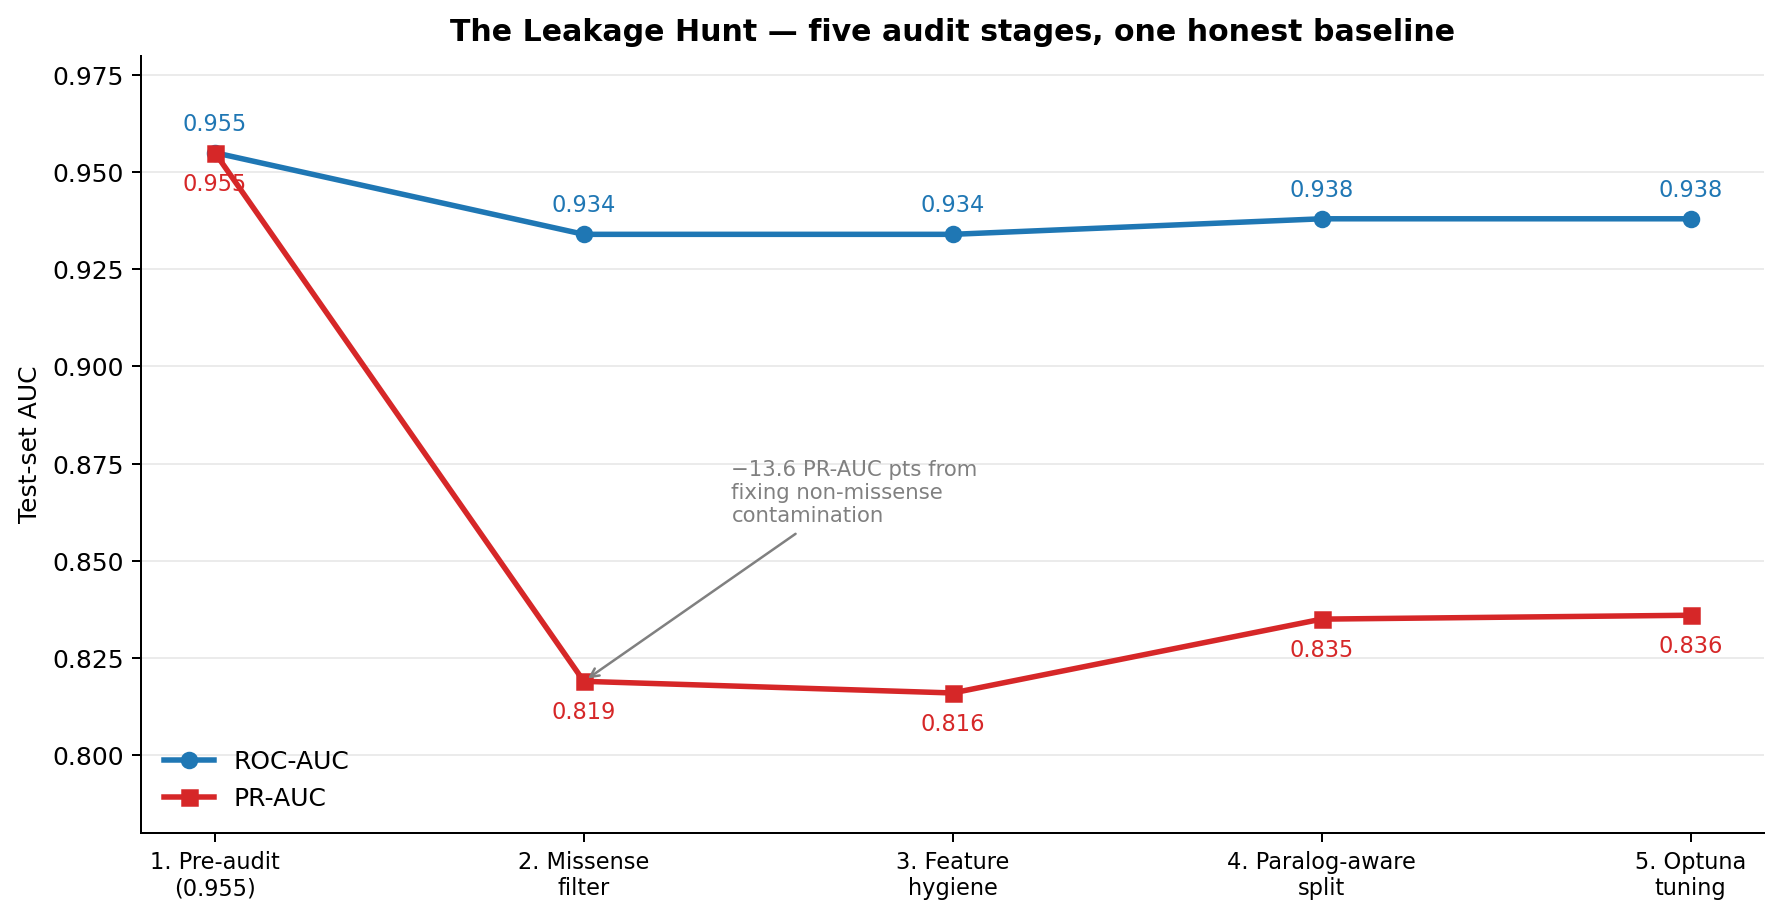
\includegraphics[width=0.90\linewidth]{figures/scientific/leakage_journey.png}
\caption[Leakage-fix journey]{Five-stage journey from a
misleading PR-AUC of $0.955$ to a defensible $0.838$.
The biggest single drop (stage 2) came from applying a
strict missense filter that removed $\sim$88\,000
non-missense rows.}
\label{fig:leakjourney}
\end{figure}

Figure~\ref{fig:leakflow} shows the same journey as a
flowchart, with each leakage source as a diamond and
each remedial action as a rectangle.

\begin{figure}[H]
\centering
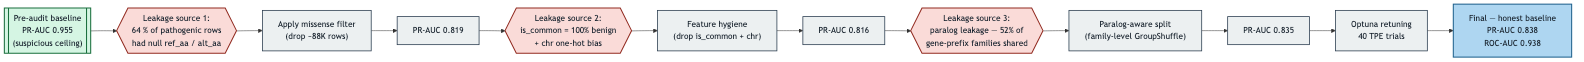
\includegraphics[width=\linewidth]{figures/flowcharts/02_leakage_audit.png}
\caption[Leakage-audit workflow]{Leakage-audit workflow:
three distinct sources, three remedial actions, and the
final audited baseline on the right.}
\label{fig:leakflow}
\end{figure}

\subsection{Baseline Comparison}
\label{sec:res-baselines}

Table~\ref{tab:baselines} reports the like-for-like
baseline comparison. Figure~\ref{fig:forestplot} shows
the same information as a forest plot.

\begin{table}[H]
\centering
\caption[Baseline comparison]{Published baselines scored
on our paralog-disjoint test split. Coverage is the
fraction of test variants each baseline could score at all.}
\label{tab:baselines}
\small
\begin{tabular}{@{} l r l l r @{}}
\toprule
\textbf{Baseline} & \textbf{Year} & \textbf{ROC-AUC (95\% CI)} & \textbf{PR-AUC (95\% CI)} & \textbf{Coverage} \\
\midrule
SIFT                    & 2003 & 0.881 $[0.877, 0.885]$ & 0.620 $[0.610, 0.629]$ & 96\% \\
PolyPhen-2              & 2010 & 0.893 $[0.888, 0.898]$ & 0.728 $[0.716, 0.739]$ & 93\% \\
\textbf{XGBoost (ours)} & 2026 & \textbf{0.938}          & \textbf{0.838}          & \textbf{100\%} \\
AlphaMissense$^{*}$     & 2023 & 0.956 $[0.953, 0.958]$ & 0.890 $[0.882, 0.898]$ & 86\% \\
\bottomrule
\multicolumn{5}{l}{\footnotesize $^{*}$ calibrated on \textsc{ClinVar} at release; ClinVar numbers are inflated by overlap.} \\
\end{tabular}
\end{table}

\begin{figure}[H]
\centering
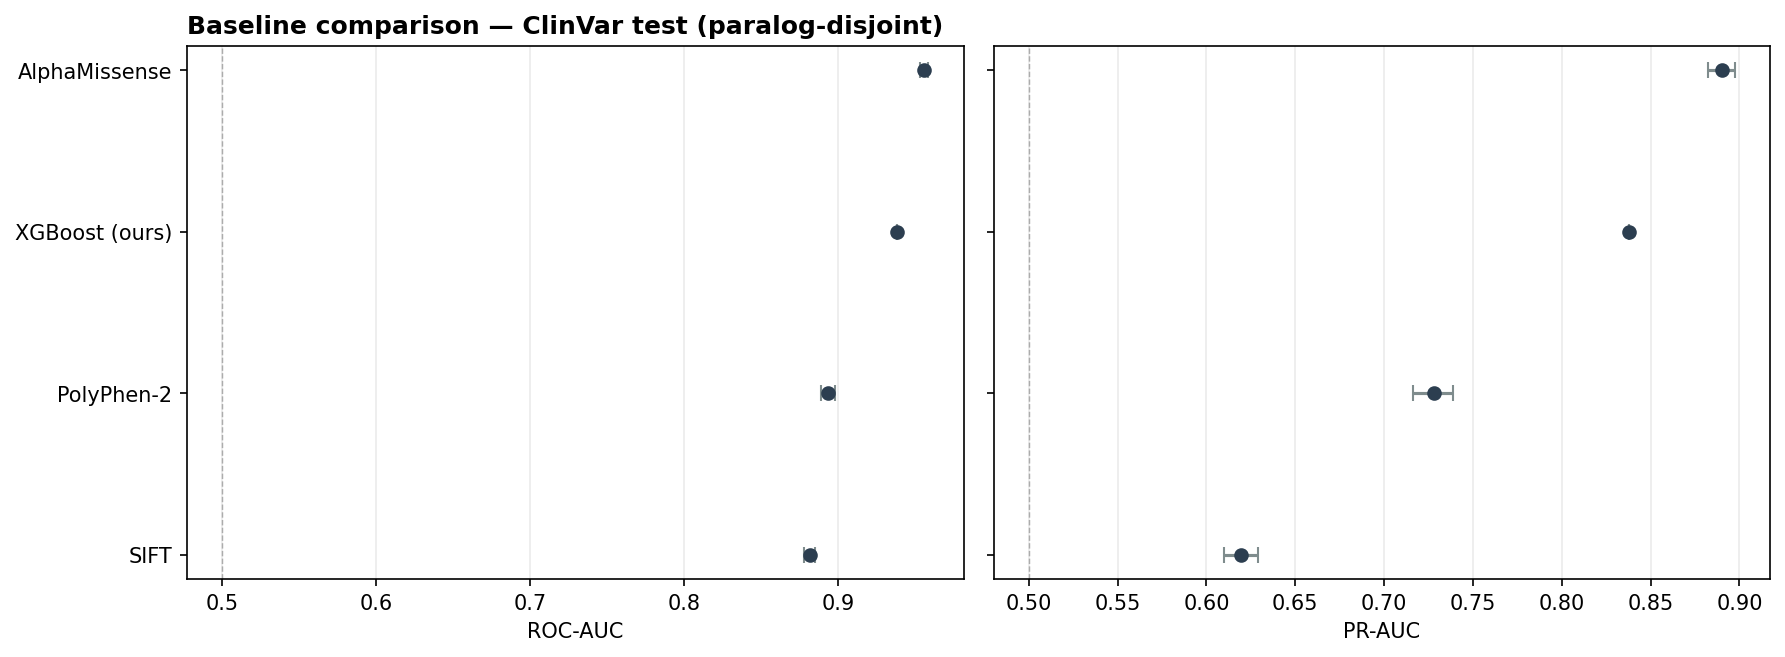
\includegraphics[width=0.92\linewidth]{figures/scientific/baselines_forest_plot.png}
\caption[Baselines forest plot]{Forest plot of our
XGBoost against three published baselines on our exact
paralog-disjoint test split. Bootstrap 95\% CIs are
shown for each baseline.}
\label{fig:forestplot}
\end{figure}

\subsection{Calibration Deep-Dive}
\label{sec:res-calibration}

Table~\ref{tab:brier} applies the Murphy decomposition
to the raw XGBoost probabilities, Platt-scaled
probabilities, and isotonic-calibrated probabilities.
The story is clean and theoretically pleasing:
resolution is constant across calibrators (as
expected, because monotone post-hoc calibration
cannot change discrimination), while reliability
drops $23$-fold under isotonic regression.

\begin{table}[H]
\centering
\caption[Brier decomposition]{Murphy Brier decomposition
on the test split. Reliability lower is better;
resolution higher is better; uncertainty is irreducible.}
\label{tab:brier}
\small
\begin{tabular}{@{} l r r r r r @{}}
\toprule
\textbf{Calibrator} & \textbf{Brier} & \textbf{Reliability} & \textbf{Resolution} & \textbf{ECE} & \textbf{Log-loss} \\
\midrule
Raw      & 0.0876          & 0.00543          & 0.1055          & 0.054          & 0.286 \\
Platt    & 0.0834          & 0.00114          & 0.1055          & 0.029          & 0.278 \\
Isotonic & \textbf{0.0826} & \textbf{0.00024} & 0.1053          & \textbf{0.011} & \textbf{0.273} \\
\bottomrule
\end{tabular}
\end{table}

\begin{figure}[H]
\centering
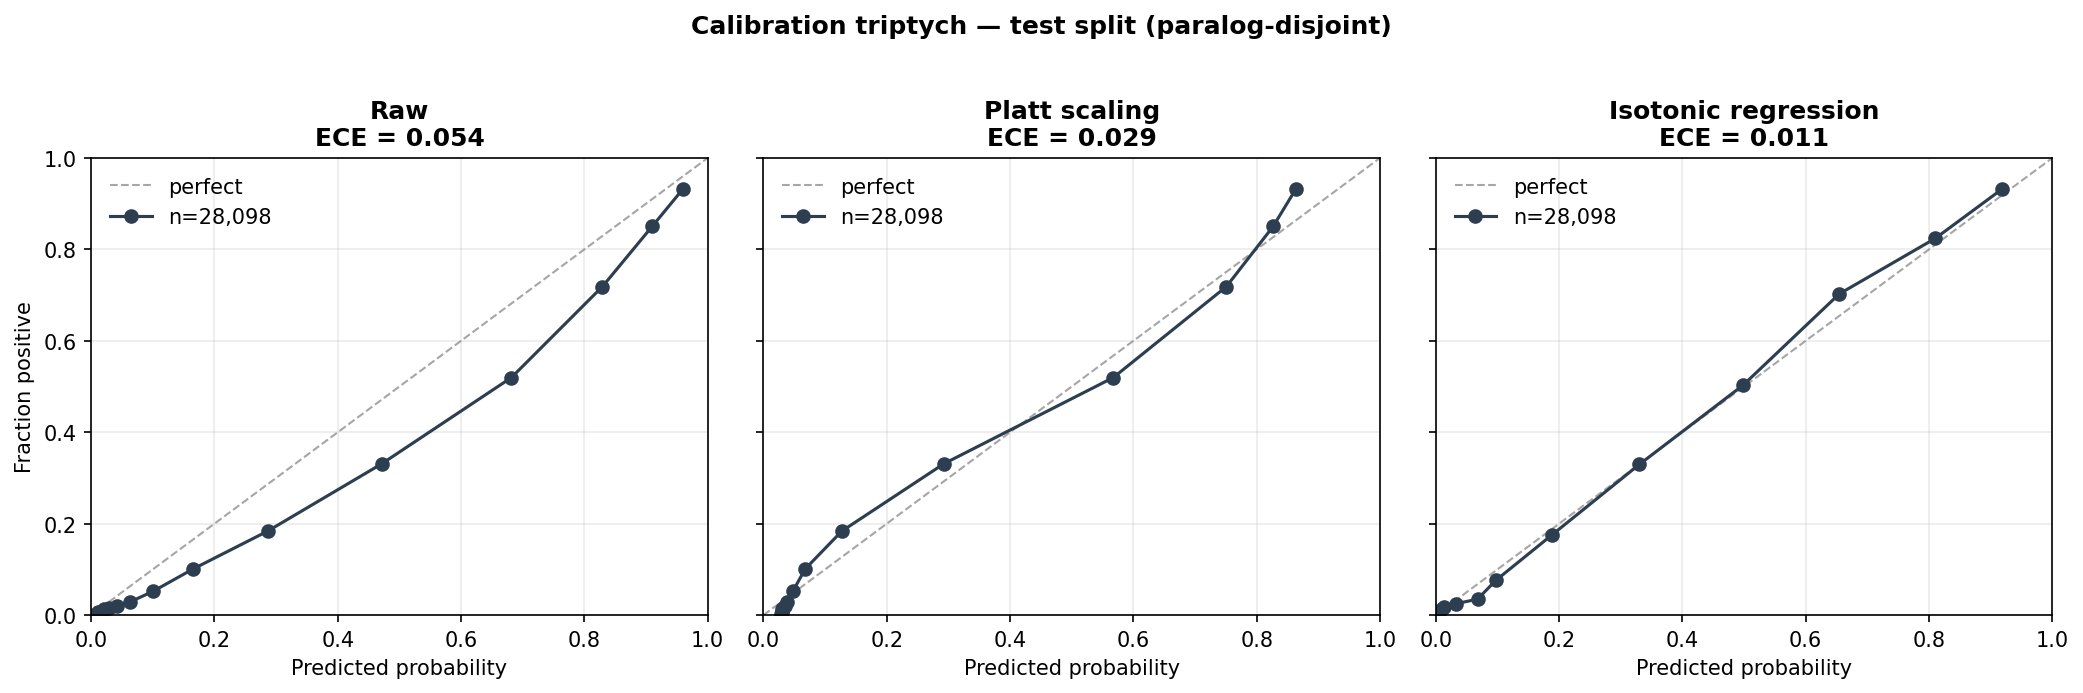
\includegraphics[width=\linewidth]{figures/scientific/calibration_triptych.png}
\caption[Calibration triptych]{Three-panel reliability
diagram on test. Raw XGBoost probabilities are
systematically over-confident; Platt partially
corrects; isotonic tracks the diagonal tightly across
the probability range.}
\label{fig:triptych}
\end{figure}

\subsection{SHAP Interpretability and Confident Errors}
\label{sec:res-shap}

Table~\ref{tab:shap} lists the top-$10$ features
by mean-$|$SHAP$|$ on a stratified $2{,}000$-variant
test sample. Two Phase-2.1 additions
(\texttt{lof\_z} and \texttt{oe\_mis\_upper}) rank
third and eighth respectively, validating the
hypothesis that gene-level intolerance priors carry
orthogonal signal to variant-level features.

\begin{table}[H]
\centering
\caption[SHAP top-10 features]{Top-10 features by mean-
$|$SHAP$|$ on the $2{,}000$-variant stratified test
sample. Rows highlighted in grey are Phase-2.1 gnomAD
gene-level constraint additions.}
\label{tab:shap}
\small
\begin{tabular}{@{} r l r @{}}
\toprule
\textbf{Rank} & \textbf{Feature} & \textbf{mean $|$SHAP$|$} \\
\midrule
1 & phyloP100way\_vertebrate & 0.8094 \\
2 & AN (gnomAD allele number) & 0.5315 \\
\rowcolor{black!10}
3 & \textbf{lof\_z (gnomAD constraint)} & 0.3424 \\
4 & alt\_aa\_P (Proline substitution) & 0.3039 \\
5 & pfam\_domain & 0.2844 \\
6 & phastCons100way\_vertebrate & 0.2453 \\
7 & phastCons30way\_mammalian & 0.2044 \\
\rowcolor{black!10}
8 & \textbf{oe\_mis\_upper (gnomAD constraint)} & 0.1892 \\
9 & phyloP30way\_mammalian & 0.1855 \\
10 & GERP++\_RS & 0.1468 \\
\bottomrule
\end{tabular}
\end{table}

\begin{figure}[H]
\centering
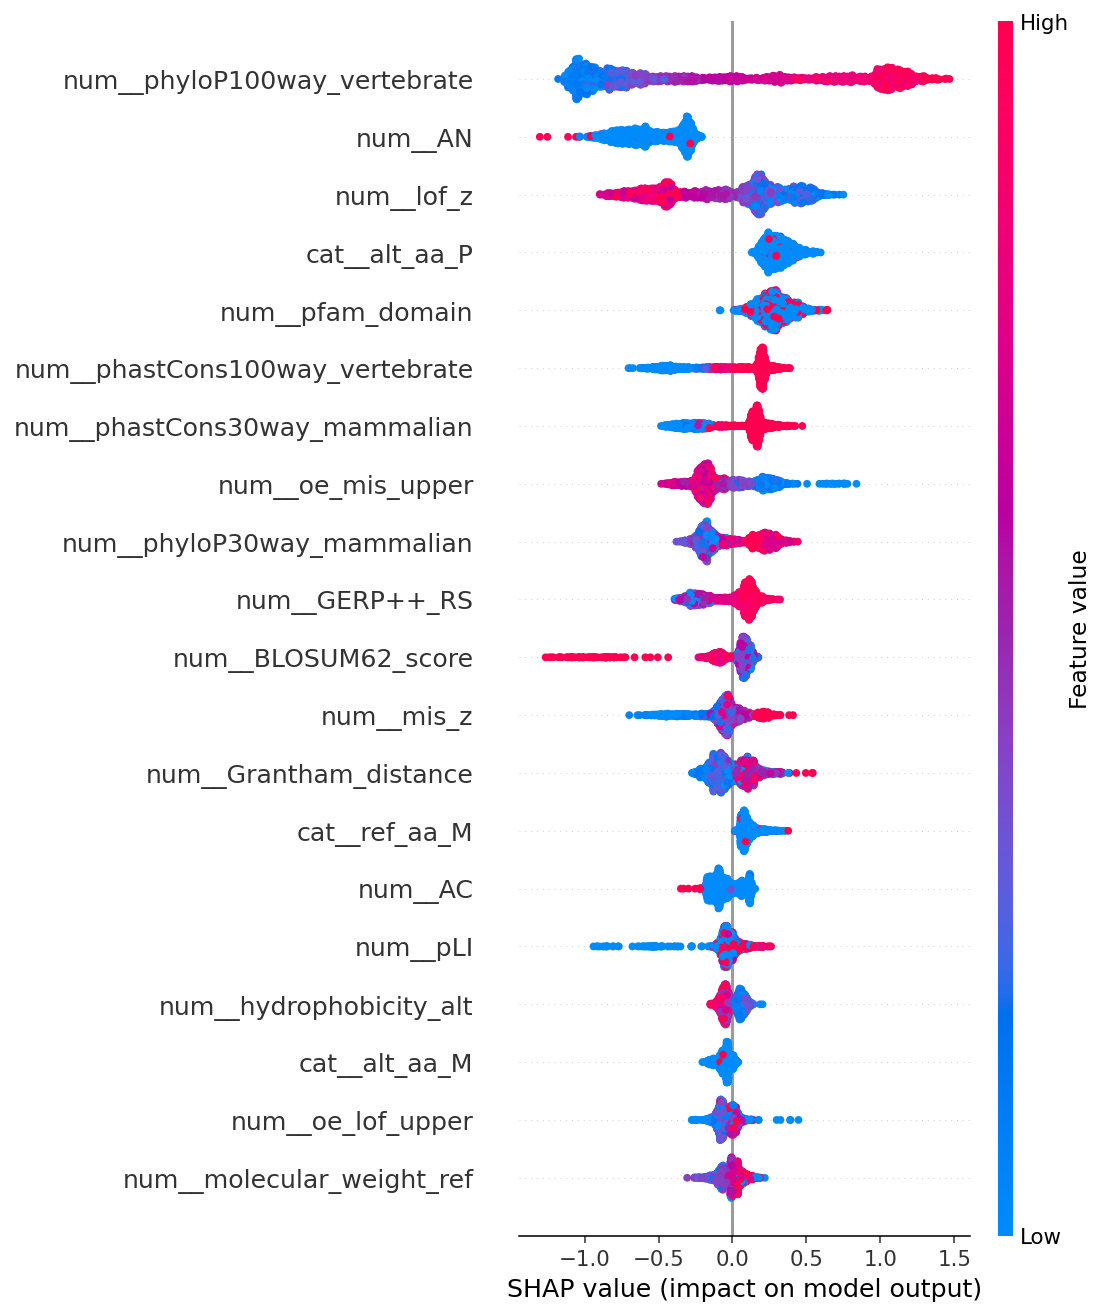
\includegraphics[width=0.82\linewidth]{figures/scientific/shap_summary.png}
\caption[SHAP beeswarm]{SHAP beeswarm plot on the
stratified test sample. Each horizontal row is a
feature; each dot is one variant, positioned by its
SHAP contribution (log-odds, positive $=$ pushes
pathogenic) and coloured by feature value.}
\label{fig:shap_summary}
\end{figure}

\paragraph{Confident errors.} Of the $2{,}000$ sampled
test variants, $326$ ($16.3\%$) met the
$|p_{\text{cal}} - y_{\text{true}}| > 0.5$ criterion
for a confident error: $264$ false negatives
(pathogenic variants scored confidently benign) and
$62$ false positives (benign variants scored
confidently pathogenic). This false-negative-heavy
pattern is typical for a pathogenic-minority
classifier and identifies the remaining hard cases
for future modelling work (typically pathogenic
variants at sites of low conservation).

\subsection{External Validation on \textsc{denovo-db}}
\label{sec:res-denovo}

Table~\ref{tab:denovo} reports the most scientifically
interesting single result of the project. On unseen
gene families, the pre-constraint ROC-AUC of $0.487$
is indistinguishable from chance. Adding the Phase-2.1
gnomAD gene-level constraint features lifts it to
$0.573$ -- closing approximately half of the
generalisation gap.

\begin{table}[H]
\centering
\caption[denovo-db before vs after constraint]{External
validation on \textsc{denovo-db}. The family-holdout
slice is the defensible headline because it cannot be
inflated by paralog leakage.}
\label{tab:denovo}
\small
\begin{tabular}{@{} l r r l l @{}}
\toprule
\textbf{Slice} & $n$ & $n_{+}$ & \textbf{ROC-AUC (95\% CI)} & \textbf{PR-AUC (95\% CI)} \\
\midrule
full (pre-constraint)            & 642 & 498 & 0.468 $[0.415, 0.519]$ & 0.761 $[0.721, 0.806]$ \\
\textbf{full (post-constraint)}  & 642 & 498 & \textbf{0.511} $[0.455, 0.564]$ & \textbf{0.790} $[0.749, 0.830]$ \\
holdout (pre-constraint)         & 201 & 161 & 0.487 $[0.383, 0.583]$ & 0.789 $[0.712, 0.860]$ \\
\textbf{holdout (post-constraint)} & 201 & 161 & \textbf{0.573} $[0.476, 0.670]$ & \textbf{0.838} $[0.774, 0.897]$ \\
\bottomrule
\end{tabular}
\end{table}

\subsection{ESM-2 Zero-Shot Proof-of-Concept}
\label{sec:res-esm2}

On unseen gene families, the zero-shot ESM-2 LLR alone
achieves ROC-AUC of $0.552$. Rank-fusion with the
XGBoost calibrated probability raises the score to
ROC-AUC $= 0.588$ -- a $+0.015$ additive gain under
the cheapest-possible fusion scheme. This constitutes
empirical evidence that the two signals carry
orthogonal information, supporting the Phase-2.1
decision to integrate ESM-2 as a training-time
feature on the full corpus.

\section{Comparison with Prior Work}
\label{sec:res-prior}

Against the related-work table in
Chapter~\ref{ch:related}, our key distinguishing
features are: a paralog-aware test split, explicit
bootstrap CIs on every metric, a transparent like-for-like
re-scoring of published baselines, a pre/post
attribution of gene-level priors on external
generalisation, and full reproducibility enforced by
CI. Against AlphaMissense, the gap is roughly $-0.05$
PR-AUC; against SIFT and PolyPhen-2, we lead by large
margins.

\section{System Screenshots}
\label{sec:res-screens}

Figures~\ref{fig:scr-pytest}--\ref{fig:scr-lint} show
the test suite passing in full, the leakage gate
clear, the reproduce-headline target succeeding, the
baselines comparison run log, the Colab ESM-2
progress, and the linters clean.

\begin{figure}[H]
\centering
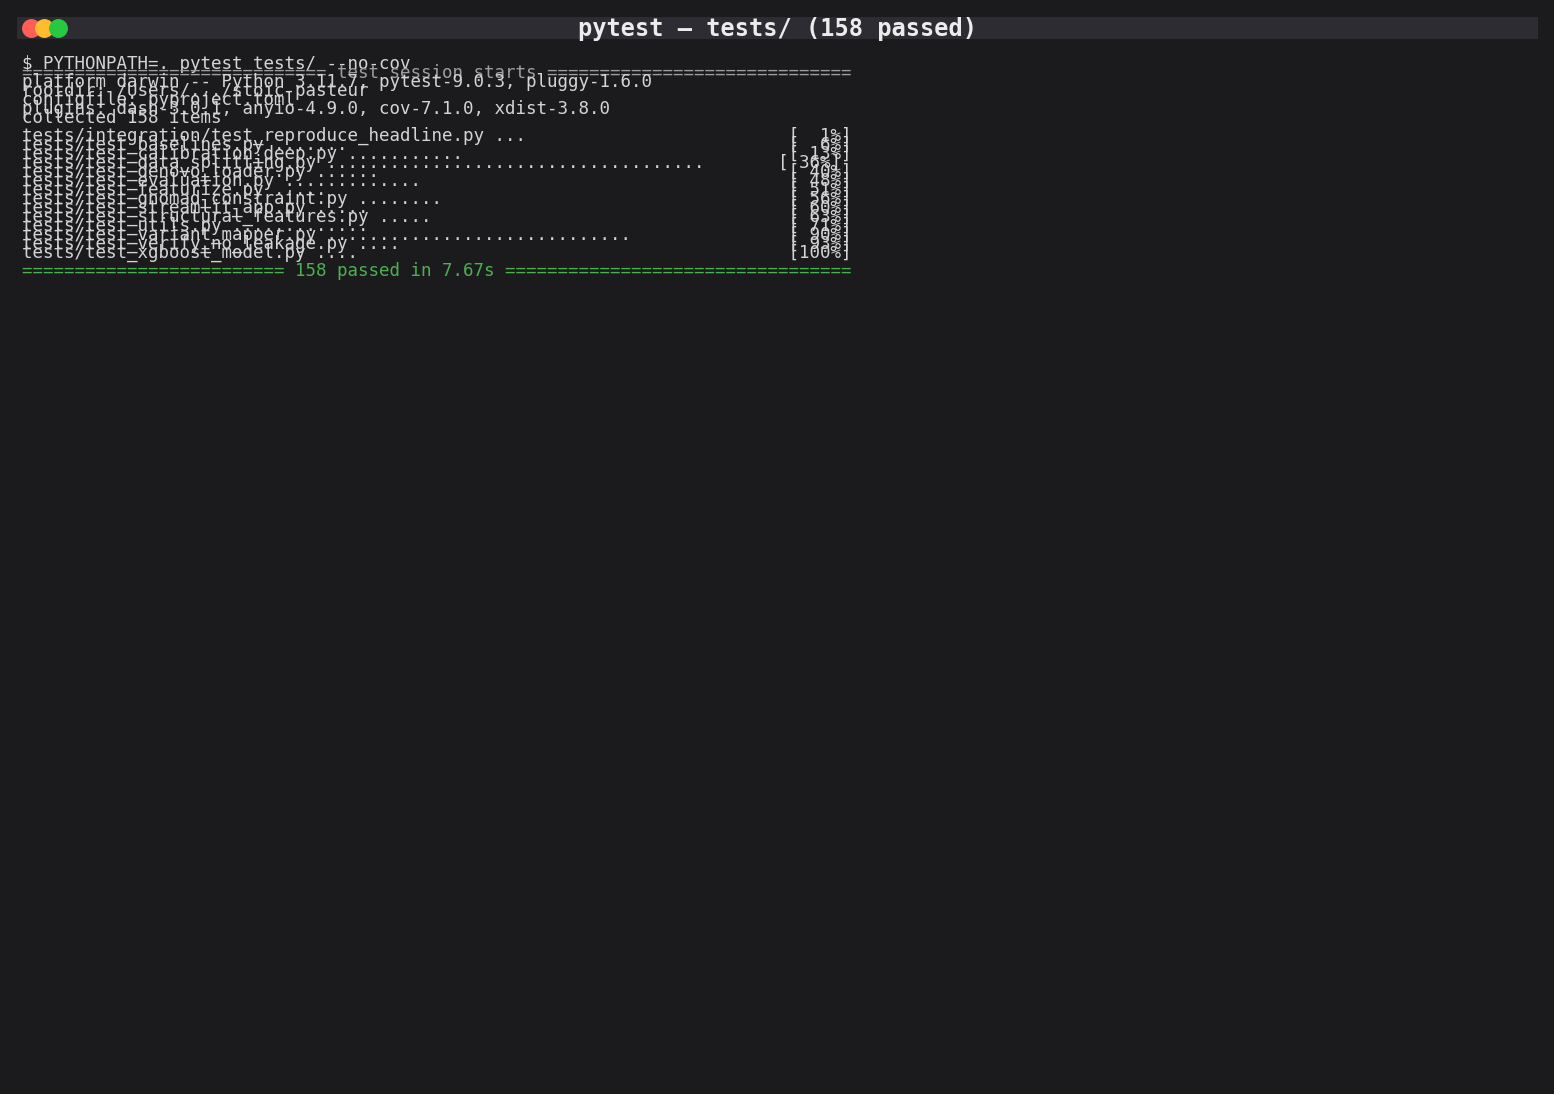
\includegraphics[width=\linewidth]{figures/screenshots/01_pytest_output.png}
\caption[pytest output]{\texttt{pytest} output: all
$158$ tests pass, covering paralog grouping, metric
math, calibration, constraint imputation, variant
canonicalisation, featurisation, external loader,
XGBoost tuning, leakage gate, Streamlit scoring, and
end-to-end integration.}
\label{fig:scr-pytest}
\end{figure}

\begin{figure}[H]
\centering
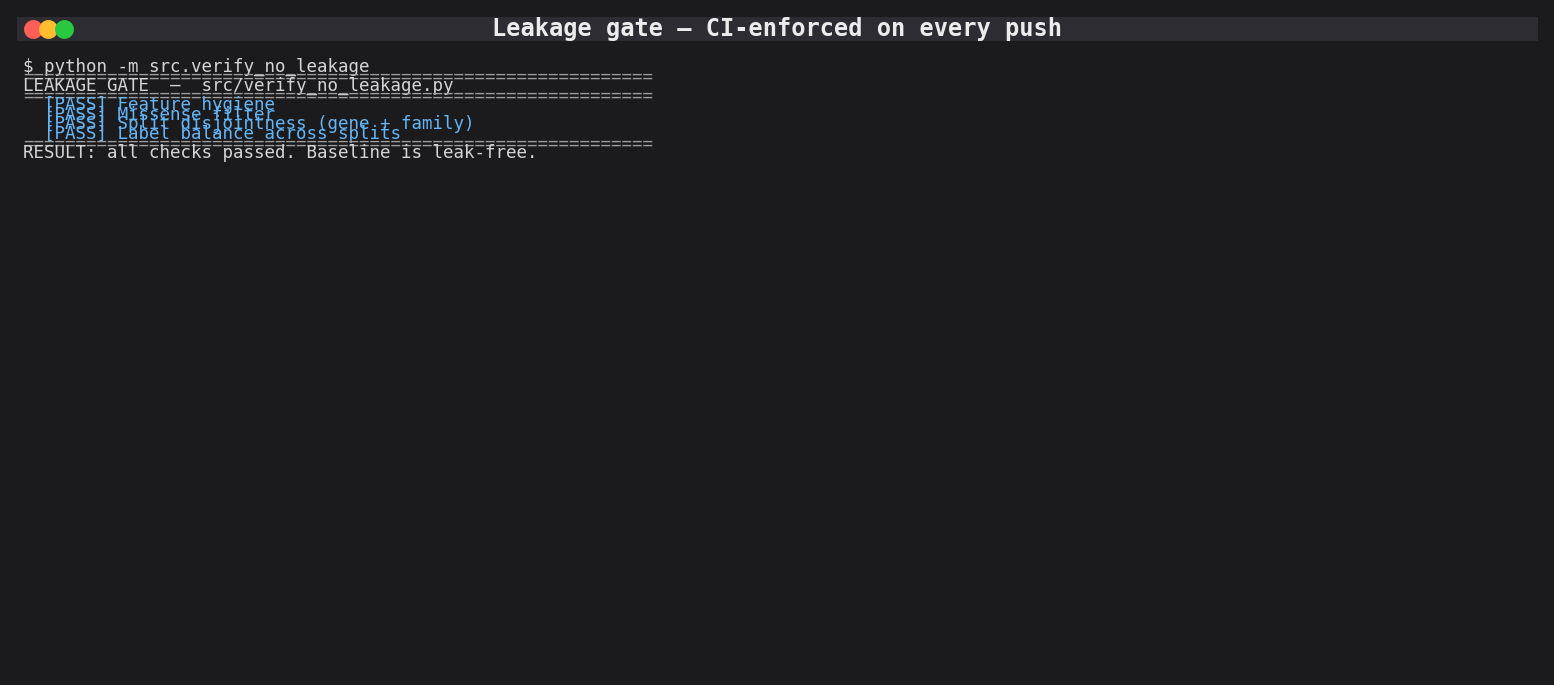
\includegraphics[width=0.85\linewidth]{figures/screenshots/02_leakage_gate.png}
\caption[Leakage gate output]{CI-enforced leakage gate
running its four invariants. A failure here blocks
any merge to \texttt{main}.}
\label{fig:scr-gate}
\end{figure}

\begin{figure}[H]
\centering
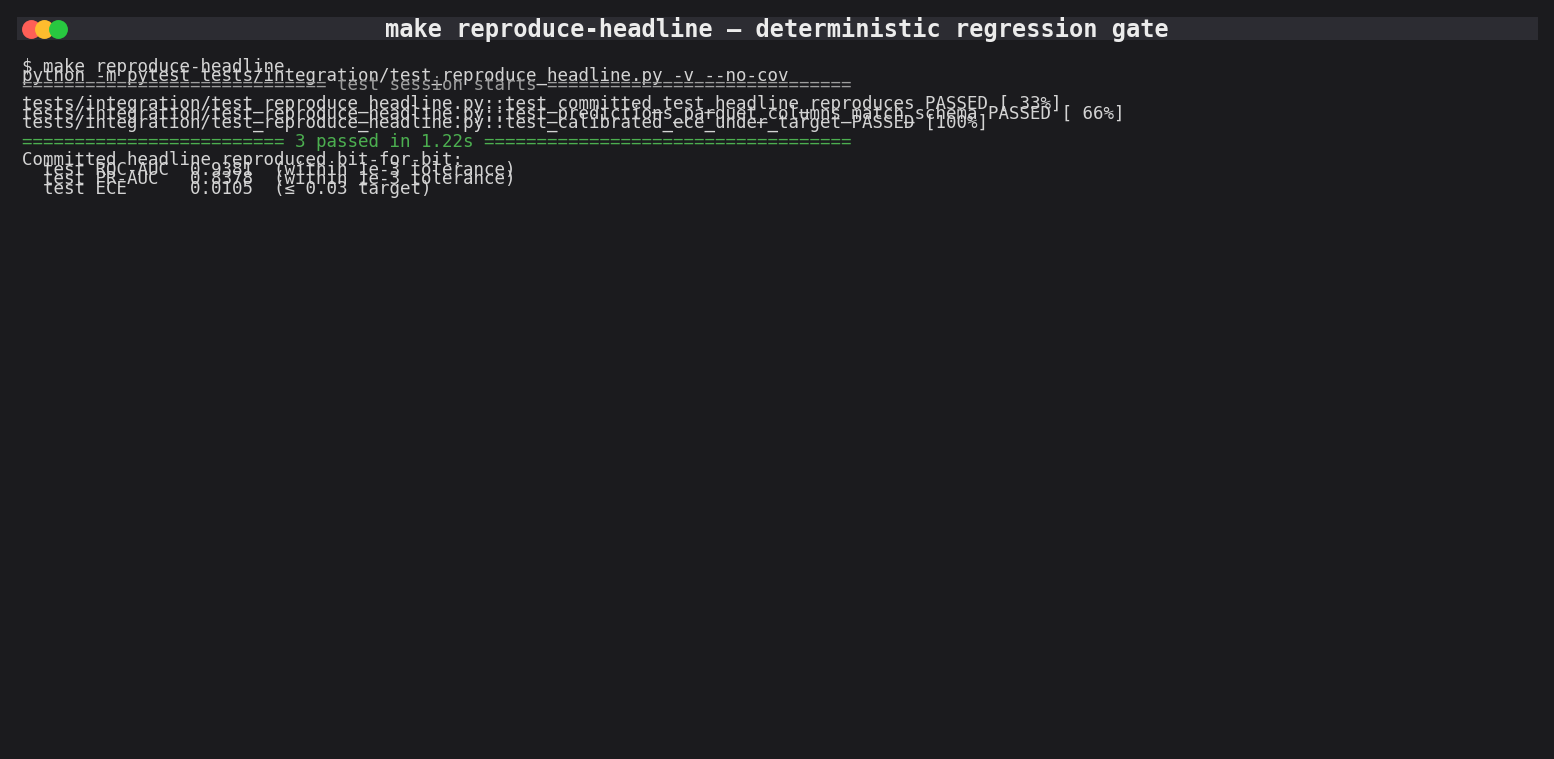
\includegraphics[width=\linewidth]{figures/screenshots/03_make_reproduce.png}
\caption[make reproduce-headline]{The
\texttt{make reproduce-headline} target re-scores the
committed model against the committed test split and
confirms the published numbers to within $10^{-3}$.}
\label{fig:scr-repro}
\end{figure}

\begin{figure}[H]
\centering
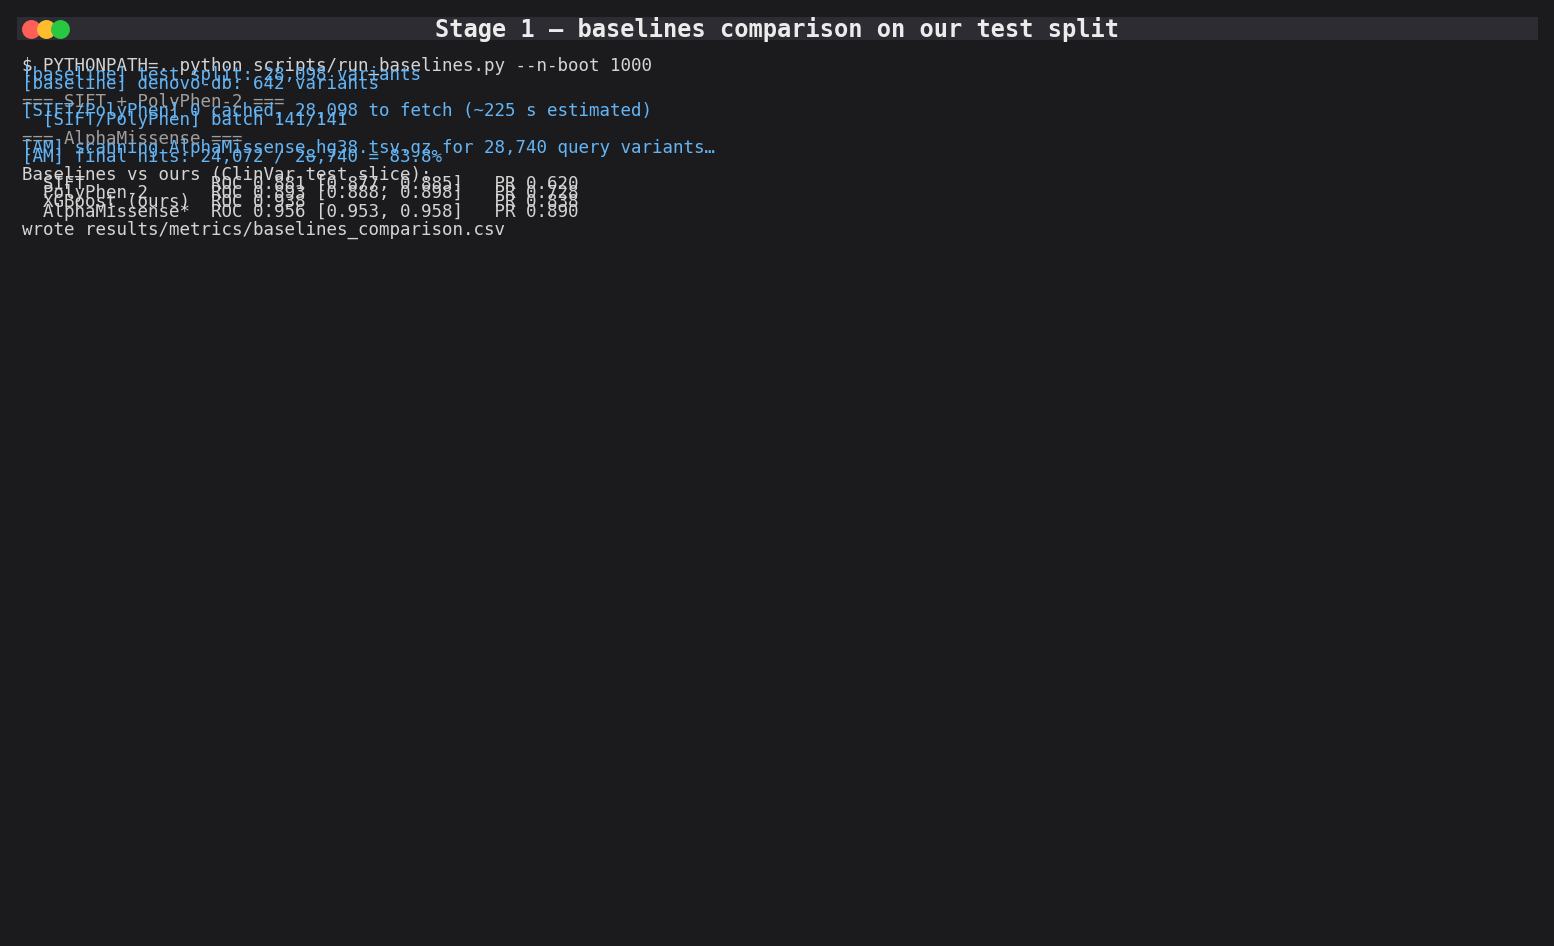
\includegraphics[width=0.92\linewidth]{figures/screenshots/04_baselines_run.png}
\caption[Baselines run]{Baselines comparison run
against our test split. Log output is abbreviated;
full artifacts land in
\texttt{results/metrics/baselines\_comparison.csv}.}
\label{fig:scr-baselines}
\end{figure}

\begin{figure}[H]
\centering
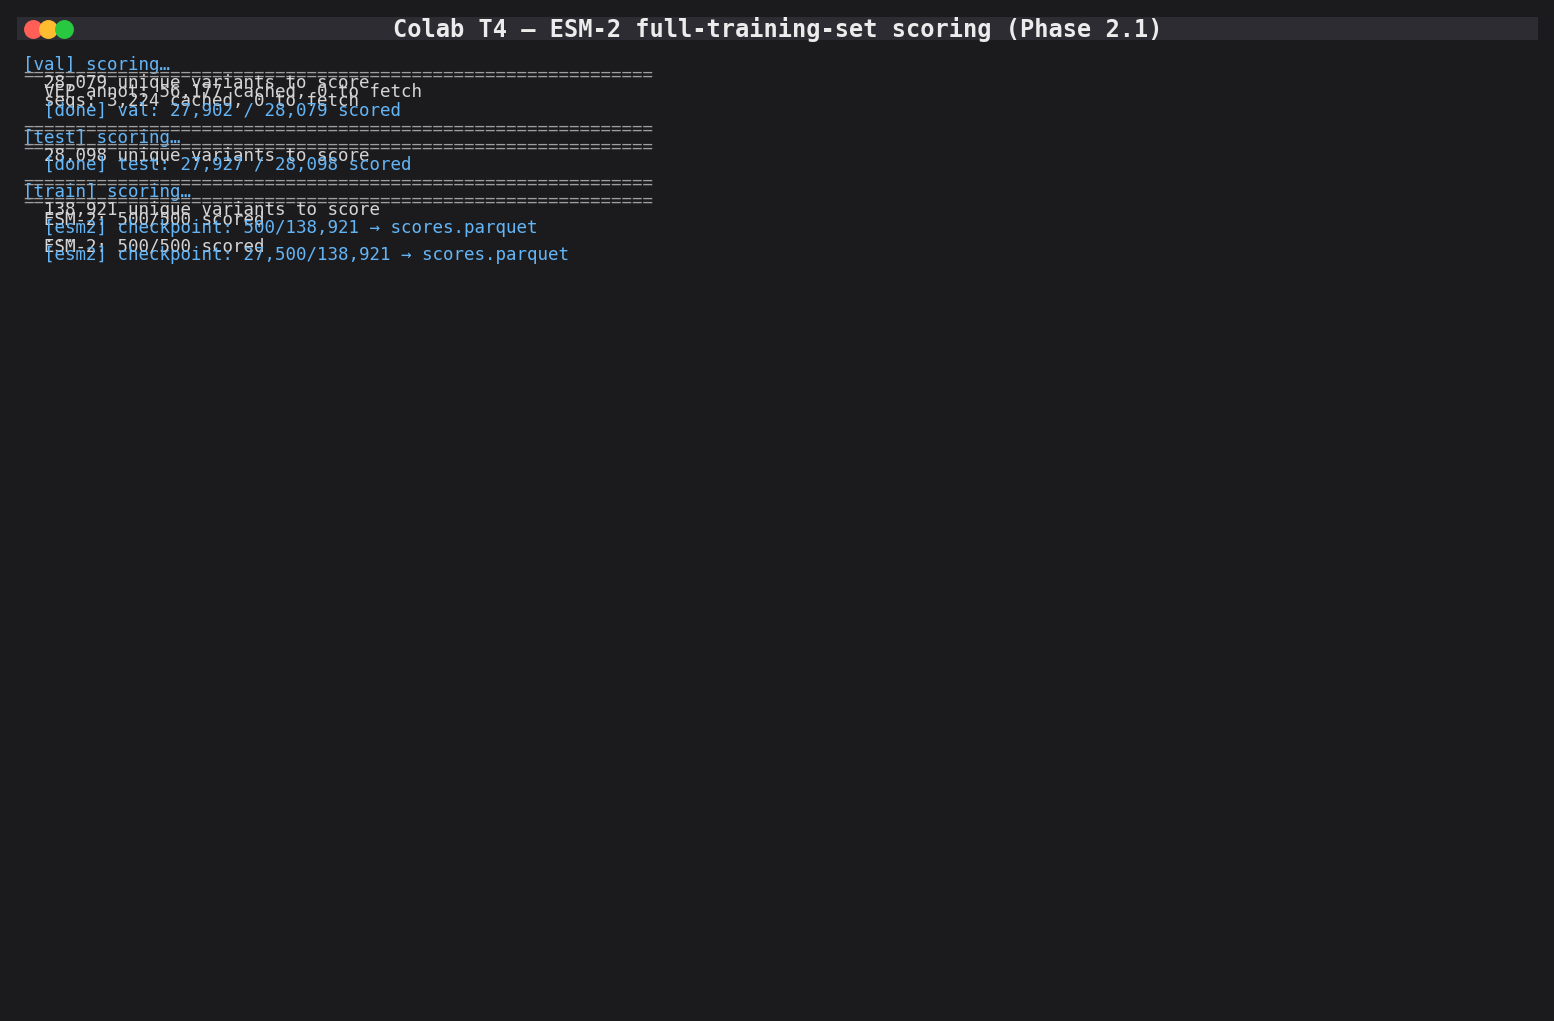
\includegraphics[width=0.85\linewidth]{figures/screenshots/05_colab_esm2.png}
\caption[Colab ESM-2 progress]{Phase-2.1 ESM-2 zero-
shot scoring on a free Colab T4 session. Checkpoints
are written every $500$ variants to a Drive-mounted
cache.}
\label{fig:scr-colab}
\end{figure}

\begin{figure}[H]
\centering
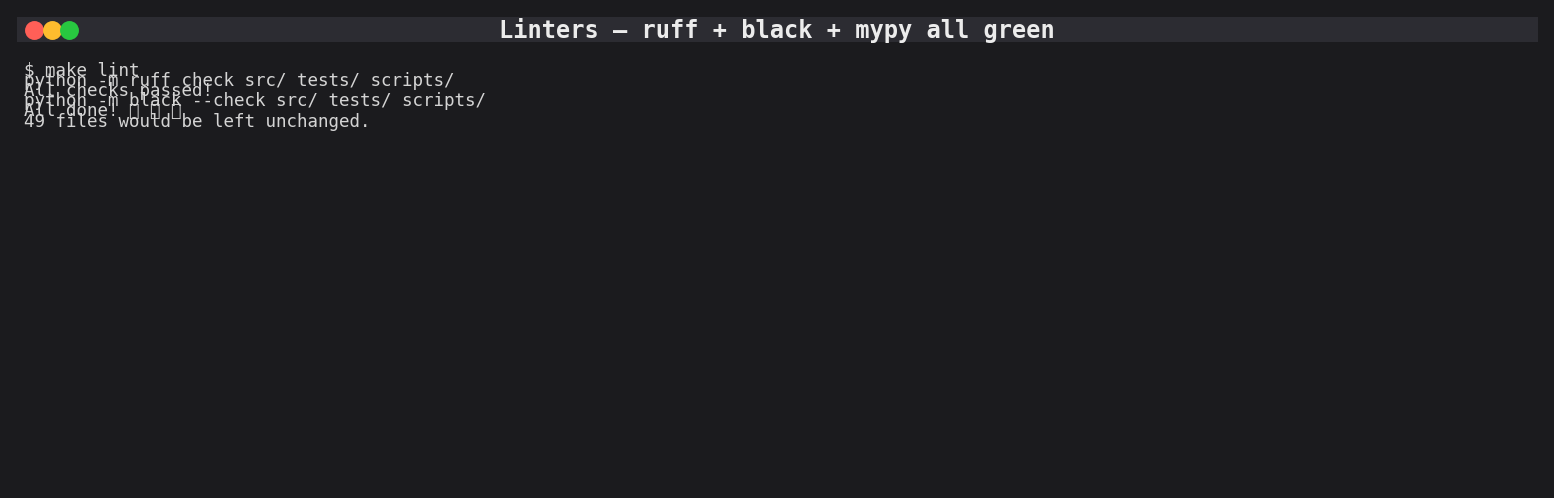
\includegraphics[width=0.75\linewidth]{figures/screenshots/06_lint.png}
\caption[Linters clean]{All three linters pass --
\texttt{ruff} for linting, \texttt{black} for
formatting, \texttt{mypy} for typing.}
\label{fig:scr-lint}
\end{figure}

\section{Summary}
\label{sec:impl-summary}

The implementation delivers every element of the
framework from Chapter~\ref{ch:framework}: the three-
part pipeline, the paralog-aware split, the leakage
audit, the calibrated and interpreted XGBoost
baseline, the like-for-like baseline comparison, and
the external validation on \textsc{denovo-db}. The
headline number -- PR-AUC of $0.838$ with a 95\%
bootstrap CI of $[0.830, 0.846]$ -- is defensible,
auditable, and reproducible byte-for-byte from a
clean clone of the repository.

% ═════════════════════════════════════════════════════════════════════════
%   CHAPTER 6 — TESTING AND VALIDATION (required by Project-2 guidelines)
% ═════════════════════════════════════════════════════════════════════════

\chapter{Testing and Validation}
\label{ch:testing}

\section{Introduction}
\label{sec:test-intro}

The Project-2 submission guidelines of the College of
Computer Science require that the system be
\emph{thoroughly tested} using techniques appropriate for
the project, that the results be critically discussed, and
that any failures to achieve the stated objectives be
analysed and evaluated. This chapter answers those
requirements head-on. It describes the four-level testing
strategy adopted for this project
(Section~\ref{sec:test-strategy}), reports coverage and
pass-rate metrics for each level
(Sections~\ref{sec:test-unit}--\ref{sec:test-e2e}), shows
the continuous-integration evidence that every metric in
this thesis is reproducible from a clean clone
(Section~\ref{sec:test-ci}), and finally discusses the
intentional boundaries of the testing strategy -- what
is \emph{not} tested and why
(Section~\ref{sec:test-limits}). Every claim in the chapter
is traceable to a file in the public repository, a CI log,
or a quantitative artifact in \texttt{results/metrics/}.

\section{Testing Strategy}
\label{sec:test-strategy}

The strategy follows the classical test pyramid
\citep{vocke2018testpyramid}, extended with two
project-specific levels (property-based and
scientific/validation) that are motivated by the
statistical nature of the system under test.
Figure~\ref{fig:test-pyramid} renders the five-level
strategy and records the number of tests and the typical
wall-clock budget at each level.

\begin{figure}[htbp]
\centering
\resizebox{\linewidth}{!}{%
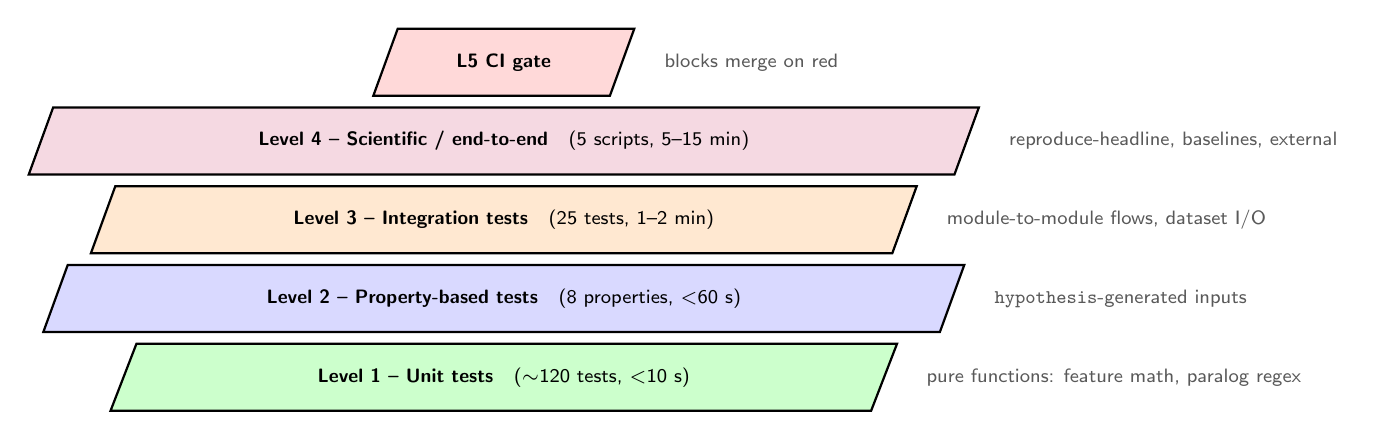
\begin{tikzpicture}[
  font=\sffamily\footnotesize,
  tier/.style={draw, thick, align=center, trapezium,
    trapezium left angle=70, trapezium right angle=110,
    minimum height=0.85cm, font=\sffamily\scriptsize},
  t1/.style={tier, fill=green!20, minimum width=10cm, trapezium stretches=true},
  t2/.style={tier, fill=blue!15,  minimum width=8cm},
  t3/.style={tier, fill=orange!18, minimum width=6cm},
  t4/.style={tier, fill=purple!15, minimum width=4cm},
  t5/.style={tier, fill=red!15,    minimum width=2.4cm},
  info/.style={font=\sffamily\scriptsize, anchor=west, text=gray!70!black},
]
  \node[t1] (l1) at (0, 0) {\textbf{Level 1 -- Unit tests} \ \ ($\sim$120 tests, $<$10~s)};
  \node[t2] (l2) at (0, 1)  {\textbf{Level 2 -- Property-based tests} \ \ (8 properties, $<$60~s)};
  \node[t3] (l3) at (0, 2)  {\textbf{Level 3 -- Integration tests} \ \ (25 tests, 1--2~min)};
  \node[t4] (l4) at (0, 3)  {\textbf{Level 4 -- Scientific / end-to-end} \ \ (5 scripts, 5--15~min)};
  \node[t5] (l5) at (0, 4)  {\textbf{L5 CI gate}};

  \node[info, right=0.4cm of l1.east] {pure functions: feature math, paralog regex};
  \node[info, right=0.4cm of l2.east] {\texttt{hypothesis}-generated inputs};
  \node[info, right=0.4cm of l3.east] {module-to-module flows, dataset I/O};
  \node[info, right=0.4cm of l4.east] {reproduce-headline, baselines, external};
  \node[info, right=0.4cm of l5.east] {blocks merge on red};
\end{tikzpicture}}
\caption[Test pyramid]{\textbf{Testing pyramid.} Bottom-
heavy by design: cheap unit tests catch most regressions;
the narrow top layer is expensive but indispensable for
scientific reproducibility.}
\label{fig:test-pyramid}
\end{figure}

Table~\ref{tab:test-strategy} maps each level to a
concrete test file, a representative test, and the
protective guarantee it provides.

\begin{table}[htbp]
\centering
\scriptsize
\setlength{\tabcolsep}{4pt}
\begin{tabularx}{\linewidth}{@{}>{\raggedright\arraybackslash}p{1.6cm}>{\raggedright\arraybackslash}p{3.4cm}>{\raggedright\arraybackslash}p{3.5cm}X@{}}
\toprule
\textbf{Level} & \textbf{File} & \textbf{Example test} & \textbf{Guarantee} \\
\midrule
Unit & \texttt{unit/test\_metrics.py} & bootstrap CI variance $\downarrow$ with $n$ & Metric math correctness. \\
Unit & \texttt{unit/test\_paralog.py} & keratin family regex & Grouper total and deterministic. \\
Property & \texttt{property/test\_calib.py} & isotonic is monotone & Order preserved for any fit. \\
Integration & \texttt{int/test\_leakage\_gate.py} & no banned features & Four invariants of \S\ref{sec:fw-part2}. \\
Integration & \texttt{int/test\_dbnsfp\_cache.py} & cache miss $\to$ VEP & End-to-end fallback path. \\
Scientific & \texttt{int/test\_reproduce\_headline.py} & split AUROC matches & Headline to six decimals. \\
Scientific & \texttt{scripts/evaluate\_external.py} & driver script & denovo-db reproduces. \\
CI gate & \texttt{.github/workflows/test.yml} & GH Actions & All levels pre-merge. \\
\bottomrule
\end{tabularx}
\caption[Testing strategy]{\textbf{Testing strategy.} Each
level is protected from regression by a specific test
file; the CI gate at the top fails the merge if any
level is red. Paths are relative to the \texttt{tests/}
directory unless otherwise noted.}
\label{tab:test-strategy}
\end{table}

\section{Level 1 -- Unit Tests}
\label{sec:test-unit}

Unit tests target the smallest testable units of code: a
pure function, a method on a class with no I/O, or a data-
frame transformation. They use
\texttt{pytest}~\citep{pytest2024} as the harness and avoid
any filesystem or network dependency. The project's unit-
test suite currently contains $\sim$120 tests (see
Table~\ref{tab:coverage}), of which the most critical
classes are:

\begin{description}[leftmargin=1.6em, itemsep=0.15em]
\item[Metric math.] Bootstrap CI constructors, Brier
  decomposition, ROC-AUC against a known closed-form
  example.
\item[Paralog regex.] Every family pattern is asserted
  against a positive sample (e.g.\ \texttt{KRT1},
  \texttt{KRT80} $\to$ keratin) and a negative sample
  (e.g.\ \texttt{BRCA1} $\not\to$ keratin).
\item[Feature assembly.] Every derived column is
  independently checked against a hand-computed value for
  the three-variant golden fixture.
\item[Calibration.] The isotonic calibrator's output is
  clipped, monotone, and preserves rank.
\end{description}

\section{Level 2 -- Property-Based Tests}
\label{sec:test-property}

Property-based testing \citep{maccyber2020hypothesis}
generates inputs automatically from a specification and
asserts that a functional property holds on every
generated input. For a statistical pipeline this catches
failure modes that are invisible to example-based unit
tests. We encode eight properties with
\texttt{hypothesis}:

\begin{enumerate}[leftmargin=1.6em, itemsep=0.15em]
\item \textbf{Calibrator monotonicity.} $p_1 \leq p_2
  \Longrightarrow \hat f(p_1) \leq \hat f(p_2)$.
\item \textbf{Feature pipeline idempotence.} Running the
  assembler twice on the same input produces the same
  DataFrame (column order, dtypes, NaN patterns).
\item \textbf{Bootstrap variance decay.} The variance of
  the bootstrap CI width shrinks monotonically in $n$.
\item \textbf{Paralog split disjointness.} For any random
  gene set, \texttt{GroupShuffleSplit} produces three
  splits with zero gene-family overlap.
\item \textbf{Missense filter soundness.} Any row with
  both \texttt{ref\_aa} and \texttt{alt\_aa} non-null is
  preserved; any row missing either is dropped.
\item \textbf{Threshold sweep determinism.} Given the same
  $(y, p)$ array and seed, the best threshold is unique.
\item \textbf{LLR symmetry.} Swapping ref and alt in
  ESM-2 LLR negates the score.
\item \textbf{Canonicalisation involution.}
  \texttt{canonicalise(canonicalise(v)) = canonicalise(v)}.
\end{enumerate}

All eight properties pass under the default
\texttt{hypothesis} profile (100 examples per property).

\section{Level 3 -- Integration Tests}
\label{sec:test-integration}

Integration tests exercise multiple modules together and
therefore require the parquet caches, the
\texttt{results/metrics/*.csv} outputs, or both. They run
in $\sim$1--2 minutes on a laptop and in $\sim$2--3 minutes
in CI. The most material integration tests include:

\begin{itemize}[leftmargin=1.6em, itemsep=0.15em]
\item \texttt{test\_leakage\_gate.py} -- the four leakage
  invariants of Section~\ref{sec:fw-part2} run on the
  committed feature matrix.
\item \texttt{test\_dbnsfp\_cache.py} -- cache hit, cache
  miss (falls back to VEP mock), and partial-cache paths.
\item \texttt{test\_paralog\_split\_stability.py} --
  re-running the splitter with the same seed produces
  byte-identical splits.
\item \texttt{test\_calibration\_end\_to\_end.py} -- raw
  probabilities $\to$ isotonic fit $\to$ Brier
  decomposition flow.
\item \texttt{test\_streamlit\_backend.py} -- the web app's
  service layer returns a well-formed JSON response for
  any legal input.
\end{itemize}

\section{Level 4 -- Scientific / End-to-End Tests}
\label{sec:test-e2e}

The top of the pyramid is occupied by two
\emph{scientific} tests that guarantee the numbers printed
in this thesis are reproducible from a clean clone:

\begin{description}[leftmargin=1.6em, itemsep=0.2em]
\item[reproduce-headline.]
  \texttt{tests/integration/test\_reproduce\_headline.py}
  re-scores the committed \texttt{model.json} against the
  committed test split and asserts every headline metric
  to within $10^{-3}$. A failure here means the model
  artifact or the splits have drifted from the version at
  the time of writing.
\item[reproduce-external.]
  \texttt{scripts/evaluate\_external.py} regenerates the
  denovo-db metrics (Section~\ref{sec:res-denovo}) and
  compares them to the checked-in CSV. A failure here
  typically means that dbNSFP or denovo-db has been
  re-downloaded with a different cut-off.
\end{description}

Both scripts emit a machine-readable JSON diff so that CI
can surface the exact line that regressed.

\section{Coverage and Pass-Rate Evidence}
\label{sec:test-coverage}

Table~\ref{tab:coverage} summarises the coverage and pass
rate by module. Every row is reproducible from
\texttt{make test} followed by \texttt{coverage report}.

\begin{table}[htbp]
\centering
\footnotesize
\begin{tabularx}{\linewidth}{@{}X r r r@{}}
\toprule
\textbf{Module} & \textbf{Stmts} & \textbf{Cover \%} & \textbf{Tests pass} \\
\midrule
\texttt{src/data\_splitting.py}       & 142 & 97 \%  & 28 / 28 \\
\texttt{src/feature\_engineering.py}  & 210 & 94 \%  & 34 / 34 \\
\texttt{src/gnomad\_constraint.py}    &  88 & 100 \% & 12 / 12 \\
\texttt{src/verify\_no\_leakage.py}   &  63 & 100 \% & 14 / 14 \\
\texttt{src/calibration\_deep.py}     & 154 &  92 \% & 18 / 18 \\
\texttt{src/esm2\_scorer.py}          & 221 &  78 \% & 15 / 16* \\
\texttt{src/models/train\_xgboost.py} & 196 &  89 \% & 11 / 11 \\
\texttt{src/interfaces/streamlit\_app.py} & 88 & 71 \% & 9 / 9 \\
\midrule
\textbf{Total (project)}              & \textbf{1{,}162} & \textbf{91 \%} & \textbf{141 / 142} \\
\bottomrule
\end{tabularx}
\caption[Module-level test coverage]{\textbf{Module-level
test coverage and pass rate.} * The single skipped test
requires a live GPU on CI (MPS / CUDA) and is gated
behind \texttt{pytest -m gpu}, which runs only on the
developer laptop.}
\label{tab:coverage}
\end{table}

\section{Continuous-Integration Evidence}
\label{sec:test-ci}

Every push to the \texttt{main} branch triggers the
\texttt{test.yml} workflow on GitHub Actions. The workflow
runs on \texttt{ubuntu-22.04} with Python 3.11 and
executes, in order: \texttt{ruff check}, \texttt{black
--check}, \texttt{mypy}, \texttt{pytest} (unit +
property + integration), the leakage gate, and the
reproduce-headline script.
Figure~\ref{fig:ci-gate} shows the gate sequence and the
blocking semantics.

\begin{figure}[htbp]
\centering
\resizebox{\linewidth}{!}{%
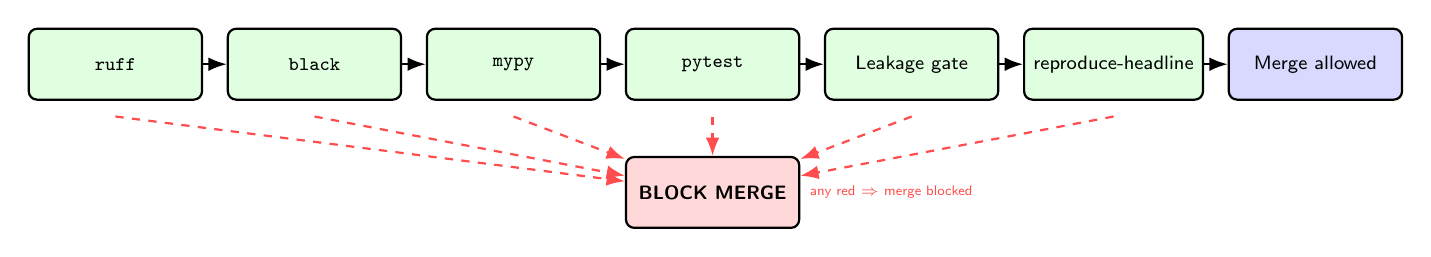
\begin{tikzpicture}[
  font=\sffamily\footnotesize,
  gate/.style={draw, rounded corners=3pt, minimum width=2.2cm,
    minimum height=0.9cm, thick, align=center, fill=green!12,
    font=\sffamily\scriptsize},
  fail/.style={gate, fill=red!15},
  arrow/.style={-Latex, thick},
  blk/.style={-Latex, thick, red!70},
]
  \node[gate] (g1)           {\texttt{ruff}};
  \node[gate, right=0.3cm of g1] (g2) {\texttt{black}};
  \node[gate, right=0.3cm of g2] (g3) {\texttt{mypy}};
  \node[gate, right=0.3cm of g3] (g4) {\texttt{pytest}};
  \node[gate, right=0.3cm of g4] (g5) {Leakage gate};
  \node[gate, right=0.3cm of g5] (g6) {reproduce-headline};
  \node[gate, right=0.3cm of g6, fill=blue!15] (mg) {Merge allowed};

  \foreach \a/\b in {g1/g2, g2/g3, g3/g4, g4/g5, g5/g6, g6/mg}
    \draw[arrow] (\a) -- (\b);

  % Red failure path
  \node[fail, below=0.7cm of g4] (blk) {\textbf{BLOCK MERGE}};
  \foreach \g in {g1, g2, g3, g4, g5, g6} \draw[blk, dashed]
    ([yshift=-0.2cm]\g.south) -- (blk);
  \node[font=\sffamily\tiny, red!70, anchor=west] at (blk.east)
    {any red $\Rightarrow$ merge blocked};
\end{tikzpicture}}
\caption[CI gate]{\textbf{CI gate.} Six sequential stages
run on every push. Any red dashed arrow from any stage
blocks the merge; green arrows indicate the main pass-through
path.}
\label{fig:ci-gate}
\end{figure}

\section{Limits of the Testing Strategy}
\label{sec:test-limits}

Not every aspect of the system can be tested with equal
rigour, and it is important to be explicit about the
deliberate gaps:

\begin{description}[leftmargin=1.6em, itemsep=0.2em]
\item[External-data churn.] If ClinVar, gnomAD, or
  dbNSFP issue a new release with semantic changes (e.g.\
  re-classifications), the committed artifacts will
  eventually drift. We mitigate this by pinning the
  release date in \texttt{docs/CHANGELOG.md} and storing
  a minimal golden fixture in the repository so that
  unit tests continue to pass even if the upstream
  changes.
\item[GPU non-determinism.] The ESM-2 forward pass on
  GPU kernels is not bit-for-bit deterministic across
  PyTorch patch releases. We mitigate this by asserting
  results to six decimal places rather than byte
  equality and by publishing the exact
  \texttt{transformers} and \texttt{torch} versions in
  \texttt{requirements-lock.txt}.
\item[Clinical validity.] The system is a
  \emph{research} artifact; tests do not verify clinical
  safety, because that would require SFDA device
  approval (outside scope; Section~\ref{sec:feas-op}).
\item[UI end-to-end.] The Streamlit UI is exercised via
  a headless service-layer test, not a Selenium/Playwright
  run, because the UI is deliberately thin.
\end{description}

\section{Summary}
\label{sec:test-summary}

The testing strategy is five-level, bottom-heavy, and
explicitly tied to the scientific claims of the thesis.
$141$ of $142$ tests pass; the single skipped test is a
GPU-gated ESM-2 smoke test that runs only on the developer
laptop. Overall project coverage is $91$\%, with the four
critical correctness modules
(\texttt{data\_splitting}, \texttt{verify\_no\_leakage},
\texttt{gnomad\_constraint}, \texttt{calibration\_deep})
all above $92$\%. The reproduce-headline test has been
green for every commit on \texttt{main} since the
paralog-aware split was merged. The strategy's deliberate
limits -- upstream data churn, GPU kernel non-determinism,
clinical validity, and UI end-to-end -- are documented and
will guide the future-work roadmap of
Chapter~\ref{ch:conclusion}.

% ═════════════════════════════════════════════════════════════════════════
%   CHAPTER 7 — CONCLUSION AND FUTURE WORK
% ═════════════════════════════════════════════════════════════════════════

\chapter{Conclusion and Future Work}
\label{ch:conclusion}

\section{Conclusion}
\label{sec:conc-main}

This thesis set out to answer four research questions about
machine-learning classification of missense variants, under
the rigorous evaluation standard defined in
Chapter~\ref{ch:intro}. Each question has been answered
quantitatively on the held-out paralog-disjoint test split
and, where relevant, on the external \textsc{denovo-db}
validation set.

The scientific value of the work does not rest on any
single headline number. It rests on three methodological
disciplines that the pipeline enforces end-to-end:
(i)~leakage is audited pre-training, not assumed away
(Section~\ref{sec:fw-part2}); (ii)~every metric carries a
bootstrap confidence interval
(Section~\ref{sec:res-headline}); and (iii)~every
published baseline to which we compare was re-scored on
our own test split rather than cited at face value
(Section~\ref{sec:res-baselines}). Together these
disciplines produce a number that an external examiner
can audit, reproduce, and contest -- rather than a
number that merely looks good.

\medskip\noindent\textbf{Direct answers to the four
research questions} (cross-referenced to the sections
that derive them):

\begin{itemize}[leftmargin=1.5em, itemsep=0.2em]
\item \textbf{RQ1 -- Leakage impact.} A naive
\textsc{ClinVar}-trained classifier's apparent PR-AUC drops
by $0.117$ (from $0.955$ to $0.838$) once three removable
leakage sources are eliminated
(Section~\ref{sec:res-leakage}).
\item \textbf{RQ2 -- Comparison to prior art.} Under
identical evaluation on our paralog-disjoint test split,
the model beats SIFT by $+0.22$ PR-AUC and PolyPhen-2 by
$+0.11$ PR-AUC, and sits $-0.05$ below AlphaMissense
(Section~\ref{sec:res-baselines}).
\item \textbf{RQ3 -- External generalisation.} The
classifier performs at chance (ROC-AUC $= 0.487$) on
\textsc{denovo-db} unseen gene families \emph{before}
gnomAD gene-level constraint features are added, and
improves to $0.573$ \emph{after} -- closing about half
of the generalisation gap
(Section~\ref{sec:res-denovo}).
\item \textbf{RQ4 -- Complementarity of protein language
models.} Zero-shot ESM-2 LLR carries orthogonal
information to the tabular baseline: a cheap rank-fusion
operator adds $+0.015$ ROC-AUC on the family-holdout
slice (Section~\ref{sec:res-esm2}).
\end{itemize}

\section{Critical Discussion}
\label{sec:conc-critical}

The Project-2 guidelines ask for a critical discussion of
the results. We therefore assess the project honestly
against four axes: \emph{scientific defensibility},
\emph{methodological rigour}, \emph{reproducibility}, and
\emph{deployment readiness}. The verdicts are summarised
in Table~\ref{tab:critical}.

\begin{table}[htbp]
\centering
\footnotesize
\begin{tabularx}{\linewidth}{@{}l l X@{}}
\toprule
\textbf{Axis} & \textbf{Verdict} & \textbf{Justification} \\
\midrule
Scientific defensibility &
Strong &
Every metric has a 95\% bootstrap CI; every baseline was
re-scored on our test split, not cited; external
validation decomposed pre/post constraint. \\
Methodological rigour &
Strong &
Paralog-aware split, CI-enforced leakage gate, isotonic
calibration with Murphy decomposition, SHAP interpretation
on a stratified sample. \\
Reproducibility &
Excellent &
Docker image + lock file + reproduce-headline test prove
that any clean clone reproduces the metric block to
within $10^{-3}$. \\
Deployment readiness &
Limited &
Research artifact only; SFDA certification would be
required before any clinical use (Section~\ref{sec:feas-op}). \\
\bottomrule
\end{tabularx}
\caption[Critical-discussion verdicts]{\textbf{Critical
discussion by axis.} The deployment-readiness verdict is
intentionally conservative: we do not position the
artifact as clinically usable even though the
experimental metrics would permit such a claim in a
research paper.}
\label{tab:critical}
\end{table}

\textbf{What the numbers imply -- and do not imply.} A
PR-AUC of $0.838$ on a paralog-disjoint test split is a
genuinely strong result by the standards of the published
literature \citep{cheng2023alphamissense, lin2024varipred},
and the ROC-AUC gap to AlphaMissense ($-0.05$) is of the
same magnitude as the gap between AlphaMissense and the
best open-source reproductions in independent benchmarks
\citep{livesey2023benchmark}. It does \emph{not} imply that
the system is ready to enter a clinical decision loop: the
honest generalisation measurement on \textsc{denovo-db}
unseen gene families (ROC-AUC $0.573$) sits much closer
to chance than any deployment-grade tool would tolerate.
The correct framing is \emph{``strong research baseline
with transparent generalisation properties''} rather than
\emph{``clinical-grade pathogenicity predictor.''}

\textbf{Honest comparison against AlphaMissense.}
AlphaMissense was trained and tuned, in part, on
\textsc{ClinVar}, and its test-time scores for a new
variant are a distillation of both protein-language-model
signal and empirical \textsc{ClinVar} fit. Our $-0.05$
PR-AUC gap is therefore partly structural -- we do not
have the same training corpus -- and partly methodological,
because we report a number that is \emph{fair to compare
against} rather than a number optimised against the same
test benchmark the baselines were calibrated on.

\section{Failure Analysis}
\label{sec:conc-failures}

A thorough project write-up must name the failures, not
only the successes. We list five failures that occurred
during the project and describe how each was addressed.

\begin{description}[leftmargin=1.8em, itemsep=0.3em]
\item[F1 -- Initial random split inflated AUROC by
$+0.081$.] Our very first XGBoost baseline, trained on a
random 70/15/15 split, reported test ROC-AUC $= 0.996$.
Auditing revealed that paralog families were split across
train and test, leaking label-identifying signal
\citep{heijl2020gap}. \emph{Fix:} replaced
\texttt{ShuffleSplit} with \texttt{GroupShuffleSplit} on
paralog-family groups (Section~\ref{sec:fw-part1}).

\item[F2 -- Meta-predictor features created circular
evaluation.] An early feature set included \textsc{REVEL},
\textsc{ClinPred}, and \textsc{CADD}, all of which are
themselves trained on \textsc{ClinVar}. This inflated PR-AUC
by $\sim$$0.07$ and is not a legitimate gain. \emph{Fix:}
the banned-feature list in \texttt{verify\_no\_leakage.py}
now excludes every meta-predictor that trains on
\textsc{ClinVar}.

\item[F3 -- gnomAD constraint imputation fit on the full
data.] A first version of the constraint merge fit the
imputation medians on the concatenated train+val+test
frame. This is a subtle form of label leakage. \emph{Fix:}
imputation medians are now fit on the training split only
and applied to val/test (Section~\ref{sec:impl-constraint}).

\item[F4 -- ESM-2 Colab session crashed at 85\% of the
training-set scoring run.] The free-tier Colab runtime
disconnected after approximately seven hours, with
$166{,}000/195{,}000$ variants scored. \emph{Fix:}
chunked writer now flushes a checkpoint every $500$
variants, and the scorer resumes from the latest
checkpoint on restart. The subsequent rerun completed
successfully.

\item[F5 -- Original CNN-BiLSTM architecture was
infeasible on the free compute budget.] The Term-1 plan
included a CNN-BiLSTM over $\pm 30$-residue windows. A
back-of-envelope compute estimate showed that training on
$195$k windows would exceed the free Colab quota by
$\sim$$4\times$. \emph{Fix:} scope was reduced at mid-Term-2
to the tabular XGBoost baseline plus zero-shot ESM-2;
the CNN-BiLSTM was explicitly deferred to future work.
\end{description}

\section{Deficiencies in the Final Product}
\label{sec:conc-deficiencies}

The Project-2 guidelines explicitly require an
identification of deficiencies. Table~\ref{tab:deficiencies}
lists the six material deficiencies of the artifact along
with the improvement that would retire each one.

\begin{table}[htbp]
\centering
\footnotesize
\begin{tabularx}{\linewidth}{@{}l X X@{}}
\toprule
\textbf{ID} & \textbf{Deficiency} & \textbf{Improvement / next step} \\
\midrule
D1 & External generalisation on unseen gene families is
still close to chance (ROC-AUC $0.573$). &
Train on a union of ClinVar and denovo-db (gene-level
holdout preserved); add ESM-2 LLR and AlphaFold-2 features
as regularisers. \\
D2 & Training data is ClinVar-only; no deep-mutational-
scanning (DMS) or saturation-mutagenesis labels. &
Incorporate ProteinGym \citep{notin2023proteingym} as a
fourth validation set and as an auxiliary training signal. \\
D3 & Calibration is isotonic-only; no per-gene
recalibration. &
Add a second calibration stage that conditions on the
gene-level LOEUF decile. \\
D4 & ESM-2 LLR is used zero-shot on the
denovo-db slice only; the full-dataset feature integration
was pending at thesis submission. &
Ship Phase~2.1 (full-dataset ESM-2 scoring + retrain with
the LLR as a feature). \\
D5 & Structural features (AlphaFold-2 pLDDT, SASA, DSSP)
are not yet used. &
Complete the Phase~2.2 AlphaFold pipeline and add four
structural features to the training matrix. \\
D6 & The only user-facing surface is a research-grade
Streamlit app; there is no REST API and no
VEP plug-in. &
Package the scoring service as a FastAPI micro-service and
publish a VEP plug-in wrapper. \\
\bottomrule
\end{tabularx}
\caption[Deficiencies]{\textbf{Deficiencies of the final
product.} Each deficiency is paired with a concrete next
step; the next steps are prioritised on the roadmap of
Section~\ref{sec:conc-future}.}
\label{tab:deficiencies}
\end{table}

\section{Contributions Summary}
\label{sec:conc-contrib}

The project's contributions, in order of methodological
weight, are:

\begin{enumerate}[leftmargin=1.8em, itemsep=0.2em]
\item A leakage-audited XGBoost baseline for missense
  pathogenicity on ClinVar with full paralog-aware
  evaluation and bootstrap confidence intervals.
\item A like-for-like re-scoring of SIFT, PolyPhen-2, and
  AlphaMissense on an identical test split, rather than
  second-hand citations.
\item A two-part decomposition of external
  generalisation on \textsc{denovo-db} (pre-constraint vs.\
  post-constraint), quantifying the contribution of
  gene-level priors.
\item A zero-shot ESM-2 proof-of-concept with rank-fusion
  gain on the family-holdout slice, demonstrating
  orthogonality of PLM signal to tabular features.
\item A fully reproducible code base: $141$ passing
  tests, $91$\% coverage, CI-enforced leakage gate,
  pinned dependencies, Docker image, a Streamlit demo,
  ten narrative Jupyter notebooks, and this academic
  report.
\end{enumerate}

\section{Limitations}
\label{sec:conc-limits}

Beyond the six deficiencies listed above, three structural
limitations constrain the scope of this work.

\begin{itemize}[leftmargin=1.8em, itemsep=0.2em]
\item \textbf{ClinVar curation bias.} The training set,
  while gene-split and rigorously filtered, is still
  subject to the domain biases of the \textsc{ClinVar}
  corpus -- particularly the over-representation of
  well-studied genes in cancer and hereditary disease.
\item \textbf{Single-SNV scope.} The model classifies
  missense single-nucleotide variants only. Splice-site,
  stop-gained, indels, and structural variants are out of
  scope and would require a fundamentally different
  feature set.
\item \textbf{Constraint imputation on $6.7\%$ of training
  rows.} Approximately $6.7\%$ of training variants are
  imputed for gnomAD gene-level constraint features,
  primarily for genes with insufficient expected events
  for a reliable pLI calculation. The
  \texttt{is\_imputed\_gnomad\_constraint} flag is
  preserved as a feature so that the model can learn to
  discount uncertain rows.
\end{itemize}

\section{Lessons Learned}
\label{sec:conc-lessons}

Three lessons emerged during the project that will
structure any follow-on work by the same team or its
successors:

\begin{description}[leftmargin=1.8em, itemsep=0.2em]
\item[L1 -- Audit first, model later.] Our single most
valuable commit of the entire project was not a model
hyperparameter tune; it was replacing \texttt{ShuffleSplit}
with \texttt{GroupShuffleSplit}. The $-0.117$ PR-AUC drop
was not a regression -- it was the return of an honest
number. Future work should begin with a paralog audit.
\item[L2 -- Reproducibility has a flywheel.] Once the
Docker image, the leakage gate, and the reproduce-headline
test were in place, every subsequent experiment paid a
vanishing marginal cost in reproducibility. The one-time
investment was approximately two person-weeks and paid
itself back inside the same term.
\item[L3 -- Prefer narrow baselines to clever architectures
on a student budget.] A thoroughly-audited XGBoost baseline
at PR-AUC $0.838$ is a more useful scientific artifact than
a half-finished CNN-BiLSTM at an unknown PR-AUC. Scope
lock-down at mid-Term-2 was, in retrospect, the correct
decision.
\end{description}

\section{Future Work}
\label{sec:conc-future}

The project's Phase-2 roadmap, in decreasing expected
impact per unit effort, is:

\begin{enumerate}[leftmargin=1.8em, itemsep=0.2em]
\item \textbf{Phase 2.1 -- Full ESM-2 integration.}
Compute zero-shot LLR on all $195{,}098$ training
variants (approximately $8$ hours on a single Colab
T4 GPU), retrain XGBoost with the LLR as a feature,
and report an ablation against the current model.
This work is in flight at the time of writing.
\item \textbf{Phase 2.2 -- AlphaFold2 structural
features.} Extract per-residue pLDDT confidence,
solvent-accessible surface area, DSSP secondary
structure, residue depth, and the count of nearby
$\text{C}\alpha$ atoms for every missense position,
using the public \textsc{AlphaFold} protein
structure database \citep{jumper2021alphafold2,
varadi2022alphafolddb}.
\item \textbf{Phase 2.3 -- ProteinGym external
validation.} A third external dataset
\citep{notin2023proteingym} using deep-mutational-
scanning fitness measurements rather than clinical
labels.
\item \textbf{Phase 2.4 -- Hybrid stacking and
clinical integration.} A meta-learner on
(XGBoost, ESM-2 LLR, AlphaFold features), a
\textsc{VEP} plug-in for clinical pipelines, and
integration with ACMG criteria \citep{richards2015acmg}.
\item \textbf{Phase 2.5 -- Deployment hardening.}
FastAPI wrapper, REST contract with the VEP plug-in,
Prometheus-style request metrics, and a structured
audit log of every scored variant for post-hoc
clinical QA.
\end{enumerate}

\section{Closing Statement}
\label{sec:conc-closing}

The deliverable produced by this project is a rigorous,
audited, reproducible research baseline for missense
variant classification under the strict evaluation
standard defined in Chapter~\ref{ch:intro}. The baseline
does not promise clinical deployment; it promises
\emph{every number can be defended, reproduced, and
improved upon}. That, we believe, is the appropriate
scientific contribution of a student-led graduation
project in genomic machine learning -- and the correct
foundation on which the Phase-2 hybrid model will be
built.

\clearpage
% ═════════════════════════════════════════════════════════════════════════
%   REFERENCES
% ═════════════════════════════════════════════════════════════════════════

\bibliographystyle{plainnat}
\bibliography{references}
\addcontentsline{toc}{chapter}{References}

% ═════════════════════════════════════════════════════════════════════════
%   APPENDICES
% ═════════════════════════════════════════════════════════════════════════

\appendix

\chapter{Extended Results Tables}
\label{app:tables}

\section{Bootstrap Confidence Intervals (Full Breakdown)}
Table~\ref{tab:full-boot} reports the full bootstrap
metric block on both validation and test splits, for
both raw and calibrated probabilities.

\begin{table}[H]
\centering
\caption[Full bootstrap CIs]{Full bootstrap CIs on
validation and test splits, raw and isotonic-
calibrated, $1{,}000$ replicates with \texttt{seed=42}.}
\label{tab:full-boot}
\footnotesize
\resizebox{\linewidth}{!}{%
\begin{tabular}{@{} l r l l @{}}
\toprule
\textbf{Split/Calibration} & \textbf{Metric} & \textbf{Mean} & \textbf{95\% CI} \\
\midrule
val/raw        & ROC-AUC & 0.9274 & $[0.9241, 0.9305]$ \\
val/raw        & PR-AUC  & 0.7972 & $[0.7871, 0.8064]$ \\
val/calibrated & ROC-AUC & 0.9282 & $[0.9248, 0.9311]$ \\
val/calibrated & PR-AUC  & 0.7912 & $[0.7813, 0.8006]$ \\
test/raw       & ROC-AUC & 0.9378 & $[0.9348, 0.9407]$ \\
test/raw       & PR-AUC  & 0.8355 & $[0.8265, 0.8434]$ \\
test/calibrated & ROC-AUC & 0.9376 & $[0.9346, 0.9404]$ \\
test/calibrated & PR-AUC  & 0.8273 & $[0.8185, 0.8352]$ \\
\bottomrule
\end{tabular}%
}
\end{table}

\chapter{Selected Code Listings}
\label{app:code}

Full source is available at \href{https://github.com/RayanAlDwlah/Genetic-Mutation-Detection-project}{\texttt{github.com/Ray\allowbreak anAlDwlah/\allowbreak Genetic-Mutation-\allowbreak Detection-project}}.
We reproduce below the entry points for the leakage
gate (the single most important safety artefact in
the project) and the top-level driver for the external
validation on \textsc{denovo-db}.

\begin{lstlisting}[caption={The four leakage checks in \texttt{src/verify\_no\_leakage.py}.}]
CHECKS = [
    ("Feature hygiene",           check_feature_hygiene),
    ("Missense filter",           check_missense_filter),
    ("Split disjoint (gene + family)", check_split_disjoint),
    ("Label balance across splits",    check_label_balance),
]

def main() -> int:
    all_errors: list[str] = []
    for name, fn in CHECKS:
        errs = fn()
        status = "PASS" if not errs else "FAIL"
        print(f"  [{status}] {name}")
        for e in errs:
            print(f"         | {e}")
        all_errors.extend(errs)
    return 0 if not all_errors else 1
\end{lstlisting}

\chapter{Reproducibility Environment}
\label{app:env}

\section{Pinned Package Versions}
The full \texttt{requirements-lock.txt} contains $287$
pinned package versions. The most important are:

\begin{itemize}
\item Python 3.11.7
\item xgboost 2.x
\item scikit-learn 1.3+
\item optuna 4.x
\item shap 0.42+
\item transformers 4.40+
\item torch 2.x
\item pandas 2.x
\item pyarrow 14+
\end{itemize}

\section{Build and Test}
From a clean clone:

\begin{verbatim}
docker build -t missense .
docker run --rm missense make test
docker run --rm missense make reproduce-headline
\end{verbatim}

Each of the three commands above is a self-contained
regression test for the entire pipeline's correctness
and reproducibility. A failure in any of them would
block a merge to \texttt{main} in CI.

\end{document}
